\documentclass{tstextbook}

\usepackage{placeins}
\usepackage[toc,page]{appendix}

%used for subfigures
\usepackage{subcaption}

%used to wrap figures around text
\usepackage{wrapfig}

% FORMAL
% for adjustwidth environment
\usepackage[strict]{changepage}

% for formal definitions
\usepackage{framed}

% environment derived from framed.sty: see leftbar environment definition
\definecolor{formalshade}{rgb}{0.95,0.95,1}

\newenvironment{formal}{%
  \def\FrameCommand{%
    \hspace{1pt}%
    {\color{lightgray}\vrule width 2pt}%
    {\color{formalshade}\vrule width 4pt}%
    \colorbox{formalshade}%
  }%
  \MakeFramed{\advance\hsize-\width\FrameRestore}%
  \noindent\hspace{-4.55pt}% disable indenting first paragraph
  \begin{adjustwidth}{}{7pt}%
  \vspace{2pt}\vspace{2pt}%
}
{%
  \vspace{2pt}\end{adjustwidth}\endMakeFramed%
}

% include subsubsection into numbering
\setcounter{secnumdepth}{3}

% used for left/right figures
\usepackage{floatrow}

\usepackage[backend=biber, style=apa]{biblatex}
\addbibresource{bibliography.bib} 

\usepackage{enumitem}% http://ctan.org/pkg/enumitem


\begin{document}

\tsbook{iGEM Phototroph Handbook}
       {The 2021 iGEM Phototrophic Teams}
       {Cover design}
       {2021}
       {a}{a}{0.0}
       {iGEM Phototrophs}
       {a}
% =====================================================================
% ============================== CHAPTER ==============================
% =====================================================================

\chapter{Introduction}






\epigraph{The following chapter was written by Lennart Lutz \& 	Paul Goffing}{\textit{iGEM Bielefeld-CeBiTec 2021}}

\section{Motivation \& Scope} 
\textbf{Welcome dear iGEMer!}
\newline\newline
In this chapter we would like to explain to you what the iGEM Phototrophs handbook is all about. This handbook was created during a collaboration of several iGEM teams from all over the world, which worked together to create a global community of teams working with phototrophs. Since working with phototrophs inhabits some challenges, which differ from the work with heterotrophic organisms like bacteria or yeast, we worked together to identify these challenges and to try to overcome them. To organise our exchange of ideas and support, the iGEM Teams Marburg and Bielefeld-CeBiTec created a community called “iGEM Phototrophs - Overgrow the World”. This community consists of three main parts: a slack workspace to connect and communicate, a series of four meet-ups with interesting guest speakers from phototrophic synbio and the work on this handbook. The first two parts, the slack workspace and the meet-ups, were mainly meant to help out each other with their current project. The handbook is meant to transport this year’s experiences to the future generations of phototrophic iGEM teams.
\newline\newline
What we envision for the future of this iGEM Phototrophs Handbook is to be a living document, to be expanded and revised by future iGEM teams and to be a resource for help and advice for iGEM teams working with phototrophic chassis. Here we explicitly include all three groups of phototrophic chassis: cyanobacteria, algae and plants. Now, one might wonder, how can this handbook help you? Well, at first, we included information about what you should consider, if you want to work with a phototrophic chassis. Second, we included many experiences this year’s teams made with their chassis, regarding topics like acquiring organisms, cultivation, transformation and cloning. Third, we collected an almost complete list of teams which worked with phototrophs since 2015, so that you can get inspiration, ideas or find out how they solved their problems. To cover as many aspects as possible, 
\newline\newline
Many of the iGEM teams working with phototrophs from all over the world are part of our community and contributed to this handbook:

\subsubsection*{ASU - United States}
\paragraph{Genetically engineering the microalgae Chlamydomonas reinhardtii to sequester arsenic from contaminated groundwater}\mbox{} \\
Arsenic contamination in groundwater is a serious problem both in local Arizonan communities and abroad: prolonged exposure to arsenic contamination can cause cancer, vascular damage, and liver failure. This project aims to engineer the microalgae Chlamydomonas reinhardtii to sequester arsenic out of water. Metallothionein, arsenate reductase, and ferritin were integrated into the microalgae via the pASapI plasmid in varying permutations. The plasmid rescues function of the photosystem II gene, leveraging the ability to photosynthesize as a selective trait. Metallothionein and ferritin bind the two most common forms of arsenic: arsenite and arsenate, respectively. Arsenate reductase catalyzes the reduction of arsenate to arsenite, allowing for the ultimate sequestration of the toxic metal to occur in the chloroplast. Transformed algae were incubated with multiple concentrations of arsenic-contaminated media and the final concentration of arsenic after 2-3 days of exposure was measured using ICP-MS to quantify uptake efficacy.

\subsubsection*{Aboa - Finland}
\paragraph{The Lac Case - Utilization of laccases for pharmaceutical waste detoxification}\mbox{} \\
Pharmaceutical waste is one of the most deleterious pollutants in the Baltic Sea. Especially the non-steroidal anti-inflammatory drug diclofenac is causing severe harm to this delicate ecosystem. The current removal efficiency of diclofenac is only 27\% at our local wastewater treatment plant. The project objective was to contribute to the development of a microbial wastewater treatment system for the detoxification of this compound. The approach was to overexpress and extract three heterologous laccases, specific enzymes which are capable of catalyzing the conversion of diclofenac into less harmful derivatives, in engineered E. coli. We were able to successfully produce and purify CotA (from B. subtilis) and CueO (from E. coli), of which CotA was shown to have catalytic activity in vitro. Implementation of this work would include the expression of this laccase in photosynthetic cyanobacteria in a closed bioreactor system, integrated as a part of the wastewater purification process.
\pagebreak
\subsubsection*{Bielefeld-CeBiTec - Germany}
\paragraph{P.L.A.N.T. Plant-based Ligand Activated Noxious agent Tracker - make the invisible visible}\mbox{} \\
As an invisible threat to the environment and human life, remnants of chemical weapons from both world wars still contaminate the soil. In Germany alone, there are over 200 suspected locations. We develop a plant-based detection system for degradation products of chemical weapons that is highly specific and allows cost-efficient screening of large areas while being easy to use. Our plant indicates the presence of toxic chemicals by changing its color to red. For this, we introduce two new reporter systems called RUBY and ANTHOS, enabling the synthesis of the plant pigments betalains or anthocyanins, respectively. If the chemical is present, it is specifically bound by a receptor, which then activates a signaling cascade, resulting in the synthesis of the pigments. Both computational design and site-directed mutagenesis are used to design new receptor proteins. In the future, our plant allows the detection of further chemicals by replacing the specific receptor.

\subsubsection*{LMSU - Russia}
\paragraph{ASCEND}\mbox{} \\
The question of food supply for the long-distance flights remains still unsolved. Moreover, onboard food production must meet restricted requirements due to the curtailed resources on the spacecraft. Сyanobacteria Arthrospira platens is a perfect candidate in this case. However, it is tasteless. A long-term ASCEND project is aimed to introduce Arthrospira platensis engineered to produce any genes of interest, and flavours in particular, as a new chassis for the synthetic biology community. We have designed and tested a special optogenetic system, which will facilitate switching between different products and help optimize growth and production conditions. Blue light induces anchoring of BcLOV4 protein in the plasma membrane and maintains culture growth, whereas far-red light induces the production of genes of interests by activating the BphP1 light-sensitive protein and forcing it to inactivate QPAS1-Gal4 repressor. This year genetic constructions were trialed in E.coli with YFP as a test gene.

\subsubsection*{Linkoping\_Sweden - Sweden} 
\paragraph{CyaSalt - A novel synthetic biology solution to the global freshwater crisis} \mbox{} \\
The world population is consistently growing and integrated agriculture is expanding consequently. As a result, the global need for freshwater is greater than ever and it continues to increase. Accordingly, the world is facing a freshwater crisis that is vastly affecting the agricultural industry in all parts of the world. CyaSalt is an innovative approach to solve this crisis. The aim of the project is to desalinate seawater in an environmentally friendly way using modified phototrophic organisms. These organisms will utilize sunlight to activate the inward-directed chloride pump, Halorhodopsin, that imports chloride ions. Sodium ions will enter via the ion channel MscL. Thereafter, the modified organisms are separated from the desalinated water by a cellulose filter. The organisms bind to the filter via a carbohydrate-binding domain on their surfaces, resulting in desalinated water free from modified bacteria. Hence, CyaSalt provides a sustainable and economically accessible freshwater source for agricultural use.
\pagebreak
\subsubsection*{MADRID\_UCM - Spain}
\paragraph{4C\_Fuels: Cyanobacterial Cyclic Carbon Capture (for sustainable bioFuel production)}\mbox{} \\
We will use cyanobacteria as living catalysts for light-driven direct carbon dioxide conversion to valuable products, upgrading the conventional biomass-based biorefineries. To do so, we will engineer the newly discovered Synechococcus PCC11801. A robust fast-growing cyanobacteria for direct sun to chemicals production. Our goal is to test the potential of photosynthetical chemical manufacturing producing n-butanol; an ideal biofuel and comodity chemical. We are implementing an artificial n-butanol biosynthetic pathway, an synthetic pathway for enhanced carbon fixation towards acetyl-CoA as central metabollite and genetic modifications for enhanced solvent tolerance. In addition we will explore cyanobacterial encapsulation in nano-structured biohybrid materials, while performing an insight into the requirements for the industrial scale-up of photobiocatalytic technology. Likewise, we will develop tools for easing cyanobacteria genetic engineering. We will develop a software for neutral integration sites identification. Also a recombination-based system for the easy generation of unmarked mutants will be developed.

\subsubsection*{Marburg - Germany}
\paragraph{OpenPlast - Establishing cell-free systems from chloroplasts as rapid prototyping platforms for plant SynBio}\mbox{} \\
Climate change is threatening many of the crops we rely on. To ensure stable food supply, engineered crops will play a major role in our future agriculture, but crop development currently takes about a decade. In our project OpenPlast, we develop cell free systems (CFS) from chloroplasts of different plants, including various crops. Showing that they can be employed as prototyping platforms to characterize genetic constructs, these systems drastically reduce testing times. We use a machine learning guided approach to optimize reaction mixture composition and create a collection of GoldenGate based chloroplast parts to be characterized in our CFS. This toolbox includes regulatory elements for chloroplasts of plants so far heavily underrepresented in the registry. After successful chloroplast transformation, we want to show that data generated in our systems is comparable to in vivo data, proving that our systems can efficiently be used as prototyping platforms for plant SynBio.

\subsubsection*{MiamiU\_OH - United States}
\paragraph{CROP: Creating RuBP Optimized Photosynthesis}\mbox{} \\
Global agricultural productivity is projected to not meet the needs of increasing populations developing higher standards of living. On a cellular level, crop yield is limited by the inefficiency of photosynthesis. Our project aims to improve this efficiency by implementing an alternative RuBP regeneration portion of the Calvin-Benson-Bassham (CBB) cycle. Two alternative pathways, which use enzymes from other reactions that act on common metabolites used in the CBB cycle, were explored first via computational modeling. Impacts on growth and reaction fluxes in silico assessed the validity of these pathways in creating a more robust photosynthetic cycle. One of these pathways which overexpresses the native enzyme transaldolase, was also assessed in vivo. Ultimately, we showed the validity of two alternative pathways in allowing a more efficient regeneration stage of the CBB Cycle. These pathways could eventually be implemented into higher plants to allow more robust cycling and therefore higher crop yield.
\pagebreak
\subsubsection*{Sorbonne\_U\_Paris - France}
\paragraph{Chlamy'n Space}\mbox{} \\
Acute or chronic exposure to ionizing radiation (UVC, gamma rays, X rays…) leads to the formation of reactive oxygen species (ROS) which affect the genome and the proteome of cells. Thus, although photosynthetic microorganisms such as Chlamydomonas reinhardtii constitute one of the main hopes for developing Bioregenerative Life-Support System during long-term space travel, their use is called into question by the decrease of efficiency of the photochemistry and by the growth arrest caused by ROS. Our project aims to make Chlamydomonas reinhardtii produce a peptide complexing with the Mn2+ ion inspired by a metabolite found in the radioresistant organism Deinococcus radiodurans and acting as an antixoidant. This study requires to demonstrate a decrease in ROS within the cell during production of the peptide and verifying the growth of microalgae cultivated in minimum medium (photosynthesis dependent growth).

\subsubsection*{Toulouse\_INSA-UPS - France}
\paragraph{Elixio, a synthetic microbial consortium for sustainable violet fragrances}\mbox{} \\
Perfumes influence perception in our daily life. Behind flowers and chic clichés, perfume reality is not so glamorous as most are issued from non-sustainable processes. This is especially true for scents impossible to extract from the so-called “mute flowers” like the violet. Our Elixio project aims to demonstrate that valuable fragrances could be easily recreated using synthetic biology, even by a small team of students. We designed a synthetic consortium involving engineered cyanobacterium and yeast and allowing a sustainable production of the violet scent molecules from atmospheric CO2. Over the summer, we successfully engineered both strains to conditionally express all the enzymes necessary to recreate the violet fragrance. Moreover, we demonstrated the production of ionones by our yeast which actually smells like violet! The Elixio project has already drawn attention from the industry and we are definitely proud of the new openings created between iGEM and the world of perfume.

\subsubsection*{Victoria Wellington - New Zealand}
\paragraph{Tropane alkaloid biosynthesis in prokaryotes}\mbox{} \\
Tropane alkaloids are plant secondary metabolites and include important medicinal compounds. Most applications are related to neurochemistry and range from the treatment of neuromuscular disorders, including Parkinson’s disease, to the use as stimulants. There is increasing need for large-scale, climate-independent, and local production of tropane alkaloids as precursors for medicinal drugs. Our goal is to remedy the impact of world crises on the cultivation and exportation of these drugs. To this avail, we aim to develop a biosynthetic route for a tropane alkaloid intermediate, tropine, in Escherichia coli and the cyanobacterium Synechococcus elongatus. To the best of our knowledge this would be the first production of tropine in a prokaryotic organism and could provide an effective and cheap alternative to current tropine production methods.

% =====================================================================
% ============================== SECTION ==============================
% =====================================================================
\pagebreak
\section{Phototrophic Chassis in iGEM}
Synthetic biology relies on the use of chassis organisms. They are re-designed, so that they gain functions the organisms wouldn’t have in a normal environment. To use an organism as a chassis in synthetic biology, it needs to be well described and easy to cultivate and have high growth rates. E. coli fulfills all of the criteria and therefore is one of the most used chassis organisms in synthetic biology. In contrast to that, synthetic biology of plants, algae and cyanobacteria is currently very rarely applied. Synthetic biologists all over the world are currently researching tools for phototrophic synbio, e.g. logic circuits, transformation methods or metabolic engineering.
\newline\newline
This situation is also reflected in iGEM, where the large majority of teams uses bacteria, mainly E. coli, as their chassis and phototrophic organisms are a quite small niche.
Due to the limited time available to most iGEM teams, it simply does not make sense for the majority of teams to invest this already very confined amount of time working on phototrophs.
\newline\newline
In 2016, the special prize “Best Advancement in Plant Synthetic Biology” was awarded for the first time to the overgrad team Cambridge-JIC, which invented a toolbox for chloroplast transformation of the green algae \textit{Chlamydomonas reinhardtii}. The first undergrad team, which won the special prize was SCAU-China. They expressed astaxanthin in rice. In 2017 this special prize was renamed to “Best Plant Synthetic Biology” and awarded every following year to undergrad and overgrad teams working with phototrophic chassis.

% =====================================================================
% ============================== SECTION ==============================
% =====================================================================

\section{Project Ideation}
As an iGEM Team it can be hard to decide for a certain project in the beginning- there are so many things that want to be thought about, among other things the organism of choice. It is likely that your team has been thinking about a project using phototrophic organisms like algae, cyanobacteria or higher plants if you are reading this. We, being iGEM phototrophic-organism-project alumnis, will try to help you decide whether a project using phototrophic organisms is right for your team.
\newline\newline
There is one thing independent from the phototrophic organism of choice: gaining the necessary knowledge. For most teams coming from a bacterial background working with phototrophic organisms - especially plants - seems deterrent at first, giving their lack of knowledge. To help with the first steps we created this handbook. Beside that it is really helpful to have local know-how like a PI working with the corresponding phototrophic organisms or a university working group.
\newline\newline
Otherwise the different phototrophic organisms require different considerations and preparations.
\newline\newline
Let's start with talking about higher plants. First of all: plants are great! Depending on your project idea you already might have stumbled upon the immense potential of plant synbio applications. 
There are the obvious improvements for agricultural purposes regarding stress tolerance, increasing their yield or adding pest resistances. 
Beside that there are also biofuel applications, implementation of new metabolite pathways and expressing therapeutics which makes plants as organisms quite versatile.
\newline\newline
When working with higher plants there are a few things to consider beforehand. The main point is time consumption since you can't just throw some cells from a cryo-stock into medium and work with them the next day as it is possible with bacteria. Acquiring plants, both from a university-intern greenhouse or growing them themselves requires a lot of time and planning ahead: when do we need how many plants? 
\newline\newline
Another point is the transformation of plant cells. We have a whole chapter dedicated to that but the short summary is that it also takes time and is a relatively big effort. The standard method for transient transformation is agroinfiltration: beforehand transformed agrobacteria are injected into the leaves of the plant, infecting the plant-cells and transforming the tissue. Stable transformation takes even more time needing several generations of plants. Fortunately  for a proof of concept transient transformation is usually sufficient.
\newline\newline
A relevant point, especially for us iGEMers is the availability of Biobricks and parts that can be used in our constructs. Plant synbio being a rather new synbio field is still lacking a lot of well-characterized and interchangeable parts. The amount of parts e.g. on \\ http://parts.igem.org/Collections/Plants is growing bigger every year but compared to other part-collections still relatively small. Additionally compatibility issues like codon optimization, genetic instability and regulatory incompatibility should be considered when creating constructs.
\newline\newline
The final point regarding the work in the lab is about evaluation. It should be considered that evaluating and analysis methods can differ from those used for microorganisms. 
\newline\newline
Depending on your project and your region it should be considered that GMO-plants outside the laboratory can be a tricky thing to justify in the human practice sub-category of iGEM and real world application will not happen in the near future. 

% =====================================================================
% ============================== SECTION ==============================
% =====================================================================

\section{Planning \& Getting Started}
In this chapter you will find further information and tips on how to organise a project with a phototrophic organism. 
\newline\newline
The first step is to acquire the strain of choice. This can be more time consuming than initially planned. Especially for experiments with higher plants it is essential to know when how many plants of what age are needed. Obviously this needs to be known a few weeks ahead. 
\newline\newline
There are generally two ways of getting hands on plants: ordering the plants from the \\(university-) greenhouse or growing them themselves.
Ordering the plants needs good communication about the age and time when they are needed. Another consideration might be the type of soil the plants are raised and how the plants are treated once delivered.
\noindent
When raising your own plants it is important to standardize the growth conditions for every plant to get an even population. The main variables are light exposure and source as well as watering and fertilizer. 
Last but not least there are different cultivation methods- in soil, in agar and in liquid, there is a separate chapter for growth and cultivation methods.
\newline\newline
If your laboratory doesn't have equipment for growing and handling plants or other phototrophic organisms, e.g. in photobioreactors, those need to be organized ahead of time, probably bought. There are online grow-shops in every region that can be used to order equipment like grow-lamps and more.
\newline\newline
When evaluating and analysing results it should be considered that protocols or necessary laboratory-devices might differ from organism to organism and may need reservation. Also asking for advice is always recommended.



% =====================================================================
% ============================== CHAPTER ==============================
% =====================================================================

\chapter{Working with Phototrophs}



%\graphicspath{{images/chap2/}}

\section{Acquiring Organisms}
\epigraph{The following section was written by Lidia Bobrovnikova}{\textit{iGEM LMSU 2021}}
\subsection{Culture Collections}
\subsubsection{Biological collections: purpose and classification}
Biological collections constitute a fundamental heritage of information and knowledge about fauna, flora, and microbiota. They specialise in maintaining and depositing both strains of microorganisms and cell cultures of macroorganisms. Biological cultures are essential in the building of knowledge based on biodiversity. Apart from that, these safe depositaries of biological materials contribute to the acquisition of taxonomic, physiological, genetic, morphological, chemical, and ontogenetic information significantly. 
\newline\newline
Overall, culture collections can be parted into two basic categories: serve collections and work collections. Serve collections possess a great financial support from the government due to their strategic role in development of scientific research and profitability in face of distribution of strains. They are equipped with fully computerised systems of data acquisition and analysis and include large collections of strains and professional curation to serve collections. Work collections often have a comparatively modest number of strains in comparison and have a simpler and non-automated maintenance. They also typically lack robust documentation, collection management, and specialized and efficient delivery service. However, work collections are of a local, regional, and sometimes national importance, fostering various forms of research development and applications of living organisms.
\newline\newline
Ideally, all living biological collections should be affiliated with the World Federation for Culture Collections (\href{http://www.wfcc.info}{WFCC}). Founded in 1963, the WFCC is an entity that collects living biological collections of all natures in the world. About 770 culture collections from 76 countries are currently registered at the WFCC International Data Centre, with varying degrees of organization and activities (research, services, comprehensive collections, professional curation, etc.). Only about 5\% of WFCC-linked collections can be classified as service collections. The WFCC holds periodic events (e.g., the 15th International Culture Collections Conference, held in Chile in November 2019), publishes documents and studies, organizes thematic meetings, and, through organized discussions among its members, establishes actions and defines standard procedures for the operation of biological collections, such as storing strains, distributing control, security procedures, organizing collections, etc. In addition, the WFCC offers a scientific advisory service to help organize malfunctioning collections.

\subsubsection{Microalgae, cyanobacteria and plant tissue culture collections}
Isolation of new strains can be a long and tough procedure. Once isolated they can be maintained without any time limits. However, this is not often the goal for researchers and organising culture collections is a solution in this case. Microalgae and cyanobacteria culture collections are laboratories specially prepared to receive and keep organisms indefinitely, but always presumably in the long term. 
\newline\newline
Culture collections of microalgae are organized mainly according to the existing strains, and secondarily by the microalgae species. This treatment results from counting each culture derived from an isolation event as a unit, regardless of the number of species involved. Thus, very specialized microalgae collections are recognized, with a very small number of species, but with many strains in cultivation. 
\newline\newline 
Overall, collections were divided by \href{https://www.elsevier.com/books/algal-culturing-techniques/andersen/978-0-12-088426-1}{(Lorenz et al., 2005)} into three categories: 
\begin{itemize}
    \item Diverse collections dedicated to research and educational purposes
    \item Collections with well-defined delimitations of species or strains for research or practical study; and
    \item Collections of genetically well-defined and stable strains (often formed by a single
species or a few species) for molecular studies, development of biotechnological applications, etc.
\end{itemize}
\noindent
There are a number of requirements for culture collections. Firstly, all cultures must propagate in aseptic conditions. Secondly, the laboratory must possess enough space for hundreds and thousands of flasks and Petri dishes and supply all the cultures with enough light, CO2, movement of flasks and temperature regimes. Thirdly, for all the strains the appropriate liquid and/or solid medium must be selected.  The lack of the aforementioned factors might cause certain strains to exhibit morphological characteristics different from those typically seen in nature (e.g., reduced size of diatom frustules, pigmentation changes, loss or reduction of cellular projections). And finally, misidentification and accidental mixing of strains should be strictly circumvented and constantly checked. 

\subsubsection{Identification of cultures}
The maintenance of multiple strains in cultures necessarily implies the existence of an adequate identification system of each component of the collection. When few strains exist in a laboratory, controlling the identification of each material is easy and often this aspect is of little importance, as one simply writes the name of the species on the culture flask. In some laboratories, identification is done by an abbreviation of the species name, followed by elements that allow the strain in question to be readily identified. Thus, hypothetically, the cyanobacterium Synechocystis pevalekii could be identified as “SYN PEV.” An isolated strain from Guarapari waters, in Brazil, could be incorporated as SYN PEV GR1, whereas a second strain of the same species isolated from the same place could later be incorporated into the collection as SYN PEV GR2. If a new strain of the same species is isolated in another location, such as Sa\~{o} Lu\'{i}s (also in Brazil), the strain could be classified as SYN PEV SL1. The date on which the culture was inoculated should be indicated on the flask and the use of a diary, in which a continuous record of routine collection maintenance activities is made, may be sufficient to keep the cultures under control. However, the more huge the collection is, the more complex the identification process becomes. 
\newline\newline
One the one hand, it is necessary to characterise a strain from the phylogenetic point of view. This can be conducted by SSU, ITS1, ITS2, 16S/18S and some other constitutive sequences analisis. SSU and 16S/18S data provide researchers with an opportunity to build a phylogenetic tree and see the percent of relatedness of the strain with other organisms. And ITS1 and ITS2 secondary structures enable us to investigate the precise difference of very relative strains. 
\newline\newline
On the other hand, a physiological and biochemical characterisation of strains can also provide us with useful data. Some culture collections not only identify new strains, but also characterise its biotechnological potential. By that growth rate and productivity on different media, a tendency to accumulate certain storage compounds (TAG, starch, etc) or production of any particular molecules is meant. 

\subsubsection{Some culture collections around the world}
Large microalgae collections are part of the reality of some countries, providing an important service to the public. Examples of such centers are the Provasoli-Guillard National Center for Marine Algae and Microbiota (NCMA) (East Boothbay, Maine, USA), Sammlung von Algenkulturen G\"{o}ttingen Universität (SAG) (G\"{o}ttingen, Germany), Culture Collection of Algae and Protozoa (CCAP) (Oban, United Kingdom), and Australian National Algae Culture Collection (ANACC) (Hobart, Australia), Collection of microalgae and cyanobacteria of the Institute of Plant Physiology RAS (IPPAS) (Moscow, Russia), among others. The aforementioned institutions function as units that centralize the national distribution of strains to users for all types of culture uses and applications. These are centers maintained with government resources, but which have the sale of strains as a source to cover (at least partially) the expenses associated with the maintenance of the collections.
\begin{itemize}
    \item \href{http://www.algalresourcescollection.com/}{Algal Resources Collection (ARC)University of North Carolina Wilmington}
\item \href{http://www3.botany.ubc.ca/cccm/}{Canadian Center for the Culture of Microorganisms (CCCM)Vancouver, Canada}
\item \href{http://www.csiro.au/en/Research/Collections/ANACC}{CSIRO Collection of Living Microalgae (CCLM)Australia}
\item \href{http://www.chlamy.org/}{Chlamydomonas Genetics Center (CGC)North Carolina, USA}
\item \href{http://botany.natur.cuni.cz/algo/caup.html}{Culture Collection of Algae at Charles University (CAUP)Prague, Czechoslovakia}
\item \href{http://www.ccac.uni-koeln.de/}{Culture Collection of Algae at the University of Cologne (CCAC)Cologne, Germany}
\item \href{http://algae.ihb.ac.cn/English/}{Freshwater Algae Culture Collection at the Institute of Hydrobiology (FACHB)}
\item \href{http://www.iam.u-tokyo.ac.jp/index.html}{Institute of Applied Microbiology (IAM)Tokyo, Japan}
\item \href{http://www.nbrc.nite.go.jp/e/}{NITE Biological Resource Center (NBRC)Chiba, Japan}
\item \href{https://www.pasteur.fr/en/public-health/crbip/distribution/pcc}{Pasteur Culture Collection of Cyanobacterial Strains (PCC)Paris, France}
\item \href{http://www.uni-goettingen.de/en/184982.htmlhttp://www.uni-goettingen.de/en/184982.html}{Sammlung von Algenkulturen (SAG)Göttingen, Germany}
\item \href{https://www.tistr.or.th/tistrnew/main/index.php}{Thailand Institute of Scientific and Technological Research (TISTR)}
\item \href{http://www.wfcc.info/}{World Federation for Culture Collections (WFCC)}
\item \href{https://www.nies.go.jp/index-e.html}{National Institute for Environmental Studies, Japan}
\item \href{https://utex.org/}{UTEX Culture Collection of Algae at UT-Austin}

\end{itemize}

\subsection{Nagoya Protocol}
\epigraph{The following section was written by the MADRID\_UCM Team}{\textit{iGEM Madrid 2021}}
\subsubsection{What is Nagoya Protocol}

\begin{wrapfigure}{r}{0.3\textwidth}
  \begin{center}
    
\includegraphics [width=50mm] {images/chap1/Working with Phototrophs/Acquiring organisms/image1.jpg}
  \end{center}
 \caption{The Nagoya Protocol was adopted during the 2010 COP10 congress.}
\end{wrapfigure}
\FloatBarrier


The Nagoya Protocol is an international treaty developed by the Convention on Biological Diversity (CBD): the international legal instrument of the United Nations for biodiversity related affairs. It was adopted in 2010, during the 10th conference of the CBD in Nagoya. However it did not enter into force till October 2014. \\ \\
The Nagoya Protocol is an international legally binding protocol on access to genetic resources and benefit-sharing. Its main objective is to define fair and equitable sharing rules for the utilization of genetic resources and their derived benefits, thus contributing to the conservation and sustainable use of biodiversity. \\ \\ 
Thus, the protocol seeks to create a transparent legal framework for access to genetic resources in each region and the fair and equitable participation in the benefits derived from their utilization. Currently the protocol has been signed by more than 150 countries, leading to the creation of specific legal procedures within each one of them for biological resources accession from either national or international entities. \\ \\
Before the Nagoya Protocol, industrialised countries had no legal obligation to ensure fair sharing of the benefits arising from the use of genetic resources. After Nagoya participating countries are obligated to take legal, administrative or policy measures to ensure compliance with legislation governing access to genetic resources and benefit-sharing in the countries providing them. This means that before Nagoya protocol there were no clear procedures that ruled the usage of native biodiversity from a region or requesting access to it. \\ \\
Eventually, the Nagoya Protocol provides a range of recommendations, tools and mechanisms provided to assist contracting Parties. Among these resources there is the recommendation for  establishing national focal points (NFPs) and competent national authorities (CNAs) to serve as contact points for information, grant access or cooperate on issues of compliance.  \\ \\
Other remarked aspects are the creation of an Access and Benefit-sharing Clearing-House to share information, the creation of infrastructure to support key aspects of Nagoya protocol implementation and the financial support for capacity-building and development initiatives through the Nagoya Protocol’s financial mechanism, the Global Environment Facility (GEF). \\ \\
To sum up, Nagoya Protocol aims to raise awareness and promote initiatives for the protection of biodiversity and fair distribution of biological resources. To do so, the protocol establishes an international legal framework that regulates not only the access to biological resources but also the fair distribution of benefits derived for its utilization. Then most of the countries will increase their interest in biodiversity protection and easing the access to its biological resources, due to the potential benefits derived from its utilization either by their own nation or other international entities. 

\subsubsection{Acquiring Novel Organisms Protected Under Nagoya Protocol}
Despite the Nagoya protocol establishes main guidelines and provides recommendations to promote ease the access to genetic resources and benefit-sharing, the final legislations are individually performed by each country, following the recommendation of Nagoya Protocol. \\ \\
After the Nagoya Protocol  entered into force, many countries started protecting their biological resources under the shield of the treaty, especially developing countries looking to secure their regional biodiversity as a potential resource of the country. This way, most of the countries developed a national legal framework to regulate the access to national biological resources and created competent national authorities for biodiversity. \\ \\
For the researcher/institution interested in working with an organism that has been discovered in a region that has decided to regulate the access under the Nagoya framework, this translates into heavy bureaucracy that sometimes can be expensive and highly time consuming. \\ \\
Despite the Nagoya Protocol establish general guidelines to generate a set of terms for a mutual agreement for access and benefit sharing, the complexity of these tramits can widely depend on the country where the organism has been discovered and the intended usage of the organism by the receiver. \\ \\
In general terms, any access request for an specific organism protected by Nagoya protocol consists in the following steps:

\begin{enumerate}
\item First, a formal request has to be submitted to the biodiversity Competent National Authority (CNA). It is common that the submission of this form usually is followed by some type of administrative taxes. This request consists on a document providing personal information as well as information regarding the biological resource access is intended to. Information that is usually required refers to .
\begin{enumerate}
\item Type of biological resource, for example bacteria, plants, soil etc...
\item Amount of resource that is required.
\item Procedure for acquiring the resource for example request to an specific culture collection, field sampling or collection and shipment by a regional collaborator.
\end{enumerate}
\item Secondly, the provided documentation is revised by the CNA. This process can take from some weeks to months. After the revision, the CNA contacts the applicants informing them if they require further clarifications about the requested biological resource and potential derived benefits from its usage by the applicants. 
\item Once the CNA has approved the initial submission, usually they provide the applicants with the official documentation to fulfill. 
It is mainly composed of a document of Mutually Agreed Terms for Benefit Sharing (MAT-BS) which summarizes all the formerly submitted information, as well as a more detailed description of what kind of research or use is going to be performed with the biological resource and which mechanisms are going to be implemented for sharing the potential benefits derived from the usage of the biological resource.
Likewise an Internationally Recognized Certificate of Compliance is usually provided. In this document a the applicant can globally demonstrate their legal compliance with
the nationally established Access and Benefit Sharing (ABS) legislation. Applicant can also define what part of the information provided in the previous documents regarding the usage of the biological resource is confidential and should not be revealed. While the MAT-BS is only accessible to the CBD (Convention for Biological Diversity) and the CNA (Competent National Authority).
\item After fulfilling the provided documentation and its revision by both parts, it must be signed according to the established procedure by the CNA. This final signing procedure usually involves specific tramits that will depend on the country providing the resource. 
\item Once the documentation has been signed by the applicant and submitted to the CNA, a second payment for the administrative taxes can be required. Once this payment is performed and received by the CNA, the responsible  CNA manager signs the documentation and forwards it to the applicant, accompanied by a final approval letter emitted by the CNA.
\item The approval letter is the final document that allows the applicant to access the biological resource. In the case of specific organisms such as cyanobacteria, microalgae or plants maintained in a culture collection, this document must be attached with in addition with the conventional documentation for requesting a strain within the collection.  It is also important to consider that most of the Mutually Agreed Terms documents specify the entity responsible for providing the biological resources to the applicant, forcing them to acquire the organism specifically from that source. 
\end{enumerate}
It is also important to remark that in the MAT-Bs a duration for the usage of the biological resource is established. This duration can be modified or extended depending on the goals of the proposed usage of the biological resource. 


\subsubsection{A real case. Accessing a Novel Cyanobacterium Strain Discovered in India}
\textit{Synechococcus elongatus} PCC11801 is a novel fast growing cyanobacteria discovered in Powai Lake from samples collected in 2015. The iGEM Team MADRID\_UCM 2021 intended to work with this Strain. The experience of this team is going to be explained below, as an example of what a procedure for accessing Nagoya protected strains can look like. 

\begin{formal}
We, MADRID\_UCM 2021 team tried to access PCC11801 directly from the Institute Pasteur. After asking the Institut Pasteur Culture Collection of Cyanobacteria (PCC) they replied that access can only be granted after receiving permission from the National Biodiversity Authority of India (NBA), the CNA of the country.  \\ \\
The process to access the strain followed the formerly described steps, where an initial form was fulfilled online and sent to the NBA. For accession to biological resources from non-Indian parties this corresponds with the Form I that can be found online in the \href{http://nbaindia.org/content/26/59/1/forms.html}{Forms Page} of NBA. Before submitting the form, a payment of 100,000 Indian Rupee is required. This payment can be performed online via a link provided during the submission procedure. (20th of March). \\ \\
After submitting the documentation the revision period started, taking one month to receive a reply from the NBA. In this reply, certain information formerly provided during the online submission was required again as well as additional personal data. After sending all the required information NBA took near 3 weeks to reply the email, requesting some additional clarifications of the provided information. Eventually, two months and a half after the online application, we received an email from NBA, providing us the official MAT-BS and IRCC documents to fulfill and duly sign (27th of May).\\ \\
After fulfilling the documentation and sending back to NBA, the took another couple of weeks to reply. In this moment they asked us for duly signing the documents in every page and sending two copies accompanied by official Indian Stamp paper. In addition a second payment of 5,000 Indian Rupees should be performed. Since Indian Stamp paper is not available in our region and we did not received information regarding how to perform the payment, we wrote an email asking for payment procedure details, as well as alternative options for Indian Stamp paper. \\ \\
The following months consisted on an exchange of several emails where the NBA mainly stated that we still needing to send two duly signed copies in Indian Stamp papers and not mentioning more information regarding the payment of the taxes. Eventually we managed to contact the person responsible for scientific affairs within the Spanish Ambassy in India. Via this diplomatic contact we eventually managed to contact the NBA and send the required documentation via the ambassy to the NBA. We also received the bank account information and payment details via this contact. \\ \\
One week after the payment of the 5,000 Rs tax, NBA sended us the receipt of the bank transfer, asking us for concept of the transfer. We discovered that from the 5,000 Rs that were sent, only 3,555 arrived. We performed a second payment by the value of 2600 Rs, expecting that despite some of the money would be “lost“ during its way, the required amount of 1445 Rs could reach NBA. After two weeks, we received a notification that only 1,248 Rs arrived, and the import of 197 Rs still required to received the approval. After asking our bank and the National Bank of India about possible commissions that we were not advised beforehand and not receiving a clear answer, we eventually found that in any transfer performed to NBA in EUR (€) the import of 15 € was charged to the transfer for currency exchange. Then we performed a final payment of 1,700 Rs and in two weeks we received the confirmation that the money arrived properly accompanied by the signed approval letter. \\ \\
The whole process took around three months, receiving the approval letter the 17th of August from the NBA. Once received we started the request of PCC11801 to the PCC, receiving the strain eventually the 1st of September. 
\end{formal}

\subsubsection{Our Conclusions}

Despite the appealing features of Novel Discovered organisms protected under de Nagoya Protocol, the required legal procedures are long and expensive. This natura make them incompatible with the reduced duration of iGEM Teams experimental research.  If you are planning to work in your (iGEM or not) project with any strain protected under Nagoya Framework, we highly recommend you to first search for similar strains with free access for research or other purposes. If you decide to access a Nagoya Protected Strain, we highly recommend you to start at least 6 months in advance the time you are planning to start working with the strain. \\ \\
Depending on the country where the strain has been discovered the bureaucracy can be more or less agile, however in any case the procedures are more laborious, expensive and time consuming than requesting a strain which is not Nagoya protected. \\ \\
In the particular case of National Biodiversity Authority of India, they usually take around one to two weeks to reply emails. Then, trying to properly prepare all the documentation and performing payments just once can speed up the tramits. \\ \\ 
We have found that any payment performed in EUR to their account in the \textit{State Bank of India} is charged a fee of 15€ by currency exchange. To avoid long waiting times we highly recommend to perform the transfer by other systems like \textit{Xoom} (Paypal Bank Transfers Service), this way the money reaches its destination with the exactly transferred import. 

\subsubsection{Further Reading}
Full Text of Nagoya Protocol Available at CBD page at: \href{https://www.cbd.int/abs/text/}{https://www.cbd.int/abs/text/} \\ \\
F.A.Q About Nagoya Protocol Available at CBD page at: \href{https://www.cbd.int/abs/about/}{https://www.cbd.int/abs/about/}


\section{Growth \& Cultivation}
\epigraph{The following section was written by members from the Bielefeld team}{iGEM Bielefeld-CeBiTec 2021}
\subsection{Higher Plants}
Growing higher plants depends on the options you have in your laboratory and the purpose of the plants. Given the rather undemanding nature of plants there are a lot of different systems in varying complexity. Here we will focus on indoor-methods since those are reproducible and suitable for S1+ plants. Independent of the used methods and materials predetermined standard conditions should be applied.
\newline\newline
The main variables are the medium (in soil, hydroponics or agar or in vitro on plates), the lighting, the temperature and, depending on the used system, the water. Optimal conditions can vary between species. 
\subsubsection{Growing in Soil}
When cultivating in Soil there are a few general things to consider. To prevent compacting of the soil and fungi growth vermiculite, perlite, or polystyrene pellets are mixed with the soil. \\
Before use the soil can be treated with pesticides to prevent plant damage through insects and also fungi growth. Autoclaving the soil is possible but not recommended because this can change the soil properties. The pots for the plants should be sterilized, especially when reused and have drainage holes.
Fertilizer can be added to the soil or the water. For watering distilled and deionised water should be used for reproducibility \parencite{Podar2012}.

\subsubsection{Hydroponics}
For a hydroponic system the seedlings can either be raised in sand that is removed once the roots are long enough or in seedling-plugs which let the roots come out at the bottom. \\
Depending on the aim of the hydroponic system containers, different in size, volume and number of plants per container can be used. The containers should be opaque and have lids to prevent algae growth, evaporation and to create appropriate conditions for root-growth. A light colour can help decrease the temperature of the liquid inside as it may heat up in greenhouses or under certain grow-lamps. \\
When using aluminum for covering, pay caution not to contact the water or to carve the plant: aluminium-salts will form and damage the plant. \\
As holders for the plants, starter plugs made from polyurethane foam, rockwool, or cotton wool can be used. Before planting the seeds the plugs should be soaked in medium to allow pH-adjustment of the plugs.\\
Aeration pumps should be added to the containers to aerate the medium solution. \\
For larger systems instead of containers pipes and a pump system that pumps medium through the pipes are possible. 
Nutrient solutions should consist of distilled and deionised water complemented with nutrients, standard nutrient solutions like \href{http://pmb.berkeley.edu/newpmb/faculty/arnon/Hoagland_Arnon_Solution.pdf}{Hoagland's solution} will work, for different species alterations can be made \parencite{Podar2012}.

\subsubsection{Growing on Plates}
For growing plants on plates, petri dishes and medium are needed. Standard medium is based on  \parencite{Murashige1962} and should be sterilized. The plates can be made like usual plates for bacteria using the plant medium. Once firm, sterilized seeds can be placed on the agar. Horizontal and vertical placing of the plates is possible, vertical placing allowing better root development \parencite{Podar2012}. 

\subsubsection{Lighting}
The other big factor in plant growing besides nutrition is the lighting. First of all a light source is needed. Maybe the greenhouse of your university can supply you with lamps or you can grow your plants directly in it, otherwise there are numerous growth shops (mainly national, in Germany and Austria e.g. \href{https://www.grow-shop24.de/}{https://www.grow-shop24.de/} ) that sell grow lamps. LED-lamps, being more efficient and burning cooler, are generally better than conventional light bulbs \parencite{Goto2012}. Depending on the size, number and age of your plants a different lighting system  might be optimal. If you have numerous plants you need a wide covering to make sure every plant gets enough light. This can be verified using a Mini-PAM to measure the fluorescence of the photosystem II in the chloroplast. \\
There are optimal lamps for young plants, for maximal growth and for flowering. The exposure time can also vary and have different influences.

\subsubsection{Temperature}
Obviously plants can grow and survive a broad range of temperatures but if optimal growth is desired and there is the possibility to regulate the temperature of the plants environment it should be done, considering every plant has an optimal growth temperature. For most applications room temperature will be fine though. \\ \\
Below you can find a collection of optimal growth conditions, nutrition etc. for different lab relevant species.

\paragraph{Arabidopsis} \mbox{}  \\
\textit{Light intensity}. Approximate 100–200 μmol/m2 s from fluorescent bulbs, although lower light intensities have also been used (e.g., 40–60 μmol/m2 s \parencite{Podar2012}). Also, higher light intensities of 250  μmol/m2 s provided by mercury vapor lamps have been reported \parencite{Arrivault2006}. \\ \\
\textit{Photoperiod}. Long days >12 h accelerate the reproductive cycle—plants grown under long day regimes produce a small biomass (few and small leaves) while development of inflorescences occurs early. One example is 16/8 h day/night regime at 23/18°C.\\ \\
Short days <12 h favor vegetative growth—a 10 h/14 h day/night regime provides a good compromise between sufficient shoot biomass production and pre-flowering growth \parencite{Gibeaut1997}. \\ \\
\textit{Temperature}. 20–22°C day/17–18°C night. The temperatures required for Arabidopsis growth depends on the ecotype. In general, temperatures around 20–22°C during the day and 17–18°C during the night are fine for any of the ecotypes. However, A. thaliana Landsberg erecta grows better at day temperature around 23°C, whereas Columbia 0 (Col 0) shows stress symptoms at this temperature \parencite{Gibeaut1997}. \\ \\
\textit{Stratification of seeds}. Arabidopsis seeds, depending on the ecotype, can germinate without stratification. However, stratification of seeds ensures a more uniform germination and therefore a better comparison of results between different lots of seeds that are used in an experiment. Stratification of seeds is performed at 4°C for 2–4 days depending on the ecotype. Three days stratification periods would suit any of the Arabidopsis ecotypes. Stratification can be performed before sowing by placing the seeds into a vial in water or after sowing by placing the plates (in vitro experiments) or the pots with soil at 4°C. Seeds can be kept at 4°C for up to a week.\\ \\
\textit{Humidity}. High humidity is required for Arabidopsis seeds to grow, e.g., 65\% \parencite{Peiter2007}, 75 \% \parencite{Gibeaut1997}, 60/75 \% day/night \parencite{Arrivault2006}. \\ \\
Soil. In general, any standard peat-based soil/compost would work for Arabidopsis. Here are two examples: GS90 (composition: peat, clay, coconut fiber, 2 g/L salt, 160 mg/L N, 190 mg/L P2O5, 230 mg/L K2O, pH 6; supplied by Werner Tantau GmbH \& Co. KG, Germany) \parencite{Koslowsky2008} and Levington F2 seed and modular compost pH 6 (Green-tech, UK). Soil is mixed 1:1 v/v with vermiculite or perlite. \\ \\
\textit{Trays/pots}. The size of trays/pots used for Arabidopsis growth depends on the number of plants that are needed for the experiment and available space for growing. In general, people use flat cell trays if individual plants are required or large trays if plants are to be pooled. For trays with individual cells or pots a square of around 7 × 7 cm works well. However smaller cells/pots (36 cells trays) also give good results. \\ \\
\textit{Containers for hydroponics}. One example would be to use a 5 L container 35  ×  35  ×  20 cm, holding up to 36 plants, with a diameter of the hole of 1.5–2.0 cm and a distance between the holes of 4–5 cm.

\paragraph{Barley}\mbox{}  \\
\textit{Light intensity}. Barley requires high light intensities and therefore the light quality can significantly influence the performance of the plants. 350–500 μmol/m2 s photosynthetically active radiation \parencite{Gries1995}, \parencite{Holme2006} is adequate.\\ \\
\textit{Photoperiod}. 16/8 h light/dark photoperiod is used most of the time for barley. \\ \\
\textit{Temperature} The regime varies between experiments and may also depend on whether the conditions in the greenhouse or growth chamber can be adapted for barley or whether other plant species are to be grown. However, keeping the temperature in the low range 10–20°C would be beneficial. High temperatures should be avoided. If plants are to be grown for the whole life cycle then $\sim$15°C/10°C day/night temperatures gives good results \parencite{Holme2006}. Other day/night temperature regimes that can be used are: 20/15°C, 20/17°C, 21/18°C, 23/17°C \parencite{Gries1995} or 24/18°C. \\ \\
\textit{Humidity}. Relative air-humidity varies between different published data, but in general is between 60 and 80 \%. \\ \\
\textit{Soil type}. There are different types of soil that can be used to grow barley, but here are three possibilities that all work well: (1) Standard sphagnum (or sphagnum mixed with polystyrene pellets in a 2:1 ratio), (2) Levington F2 seed and modular compost pH 6 (Green-tech, UK) mixed with perlite in a 3:1 ratio or (3) compost and perlite in a 4:1 ratio \parencite{Murray2004}. \\ \\
\textit{Pots size}. A 2 L pot works well. However, smaller pots (15  ×  15  ×  15 or 13  ×  13  ×  13 cm square) can also be used, but if there are no space constraints, then larger pots would work better. \\ \\
\textit{Containers for hydroponics}. The volume of the containers varies largely between experiments. In general, if the plants are to be grown in hydroponic solution up to maturity and seeds are required 1 L hydroponic solution/ plant is recommended. Alternatively smaller containers can be use such as 5 L containers that can hold up to ten plants. Diameters of the holes should be 2.0 cm and a distance between the holes of at least 5 cm \parencite{Podar2012}.

\paragraph{Rice}\mbox{}  \\
\textit{Light intensity}. Rice, like barley, requires high light intensities and therefore the light quality can significantly influence the performance of the plants. 300–500 μmol/m2 s photosynthetically active radiation \parencite{Miyamoto2001}, \parencite{MartinezAtienza2006}. \\ \\
\textit{Photoperiod}.16/8 h light/dark photoperiod is used most of the time for rice. However 12/12 h  day/night regime can also be used. \\ \\
\textit{Temperature} The regime varies between experiments. However, rice prefers higher temperatures, in general above 20°C. Some examples of day/night temperatures used are: 25/20°C \parencite{MartinezAtienza2006} or 27/22°C \parencite{Miyamoto2001}.\\ \\
\textit{Humidity}. Relative air-humidity varies between different published data, but in general is between 40 and 80 \%. \\ \\
\textit{Soil type}. There are different types of soils that can be used to grow rice; in general clay loam mineral soil should be avoided. Levington F2 seed and modular compost pH 6 (Green-tech, UK) mixed with vermiculite or perlite in a 1:1 v/v ratio works well for rice. \\ \\
\textit{Pots size}. See barley (Subheading 4.1.2). \\ \\
\textit{Containers for hydroponics}. The volume of the containers varies largely between experiments. In general, 0.4–1 L hydroponic solution/ plant is recommended (e.g., 20–24 plants/8–10 L container \parencite{Miyamoto2001} \parencite{MartinezAtienza2006}). Alternatively smaller containers can be use such as 3 L containers that can hold up to 16 plants. Diameter of the hole is 2.0 cm and a distance between the holes of at least 5 cm should be used \parencite{Podar2012}.

\epigraph{The following section was written by members of the Linköping team}{\textit{iGEM Linkoping\_Sweden 2021}}
\subsection{Cyanobacteria}
Growth of Cyanobacteria in Different Conditions
One of the disadvantages of using Cyanobacteria in research is their relatively slow growth rate with a doubling time of 3 hours. The following experiments were therefore performed on the cyanobacteria strain synechocystis sp PCC 6803 to establish optimal growth conditions. \\ \\
For evaluation of growth the optical density was measured every 24 hours at a wavelength of 544 nm. Day 0 started with a base OD of around 0.05 - 0.08, growth was evaluated respectively. \\ \\
The standard medium used for Cyanobacteria is the BG11 medium, the protocol on page (BG11 medium page) was followed. For a real life comparison the groups with autoclaved Brackish and Sea water were added, the samples were collected at the Baltic Sea Island Gotland or the west coast of Sweden near Gothenburg. 

\begin{table}[!htpb]
\centering
\caption{Different Conditions of the growth curve experiment}
\begin{tabular}{|l|l|} 
\hline
\textbf{Name} & \textbf{What is it?}       \\ 
\hline
BG11          & BG11                      \\
pH6           & BG11 at pH 6              \\
pH7           & BG11 at pH 7              \\
pH8           & BG11 at pH 8              \\
Brackish      & BG11 + 3.5\% NaCl         \\
Sea Water     & BG11 + 3.5\% NaCl         \\
Gotland       & Brakish Water autoclaved  \\
Göteborg      & Sea Water autoclaved      \\
\hline
\end{tabular}
\end{table}
\FloatBarrier

\begin{figure}[!htbp]
    \centering
    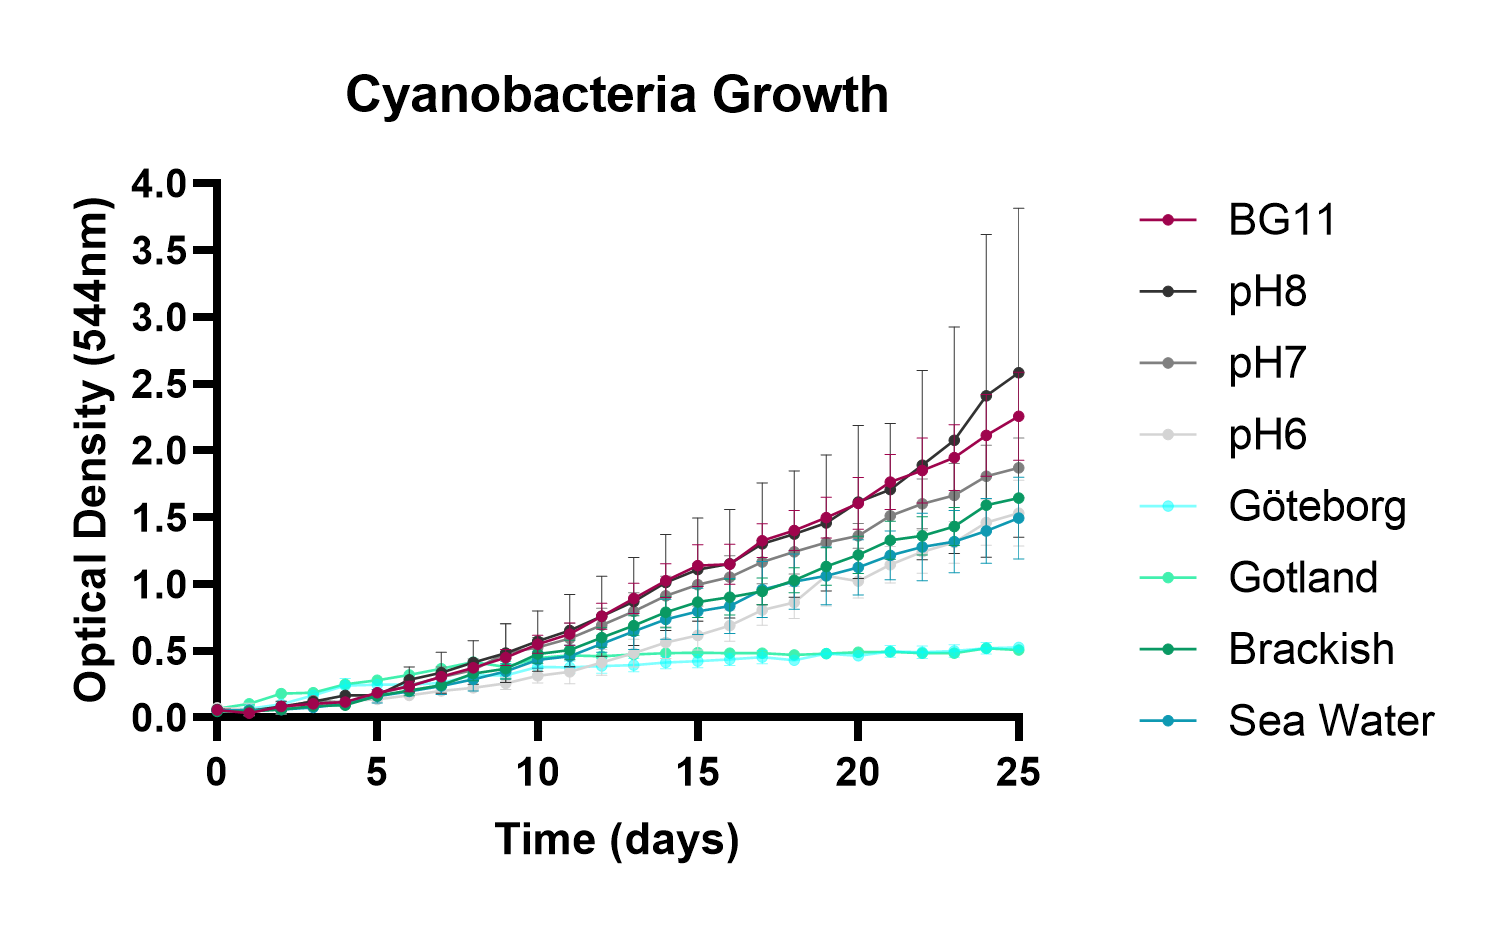
\includegraphics[width=\textwidth]{images/chap2/chap2_cyano_03.png}
    \label{fig:ch2cyano01}
    \caption{Growth curve of synechocystis in different conditions. Optical density at a wavelength of 544 nm was measured every 24 hours. Conditions are as followed: BG11 (standard medium), BG11 with different pHs (6,7,8), BG11 with different salt conditions (Brackish (1.5\% NaCl), Sea Water (3.0\% NaCl)) and water collected from the Baltic Sea and the West Coast of Sweden (Gotland, Göteborg (Gothenburg)). Error bars represent the mean +- SEM from 3 biological replicates. All growth media were autoclaved before the bacteria was added.} 
\end{figure}
\FloatBarrier
\noindent

\subsubsection{Incubator setup and lighting}
Finding standardised lighting and incubator configurations is a difficult task, but acquired data shows that with even simple setups, good growth conditions can be achieved. Normal incubators can easily be turned into incubators suitable for the growth and cultivation of cyanobacteria. In figure 2.3 below, 2 LED lamps emitting 340 lm each were installed with double sided tape in a normal incubator. This generated a light intensity gradient in the incubator, which can be seen below in table \ref{tab:gradients}. Due to the cyanobacteria growing well independently on wherever it was placed in the incubator, the conclusion can be made that the gradient had little effect on the growth condition as a whole. 

\begin{table}[!htpb]
\caption{The different gradients acquired in the incubator after the installation of the lighting}
\label{tab:gradients}
\centering
\begin{tabular}{|l|l|l|} 
\hline
\multicolumn{3}{|c|}{\textbf{Top Level }}       \\ 
\hline
Left~    & Middle   & Right                     \\ 
\hline
5700 lux & 2300 lux & 1300 lux                  \\ 
\hline
\multicolumn{3}{|c|}{\textbf{Bottom Level }}    \\ 
\hline
Left     & Middle   & Right                     \\ 
\hline
300 lux  & 300 lux  & 4000 lux                  \\
\hline
\end{tabular}
\end{table}
\FloatBarrier

\begin{figure}[!htbp]
    \centering
    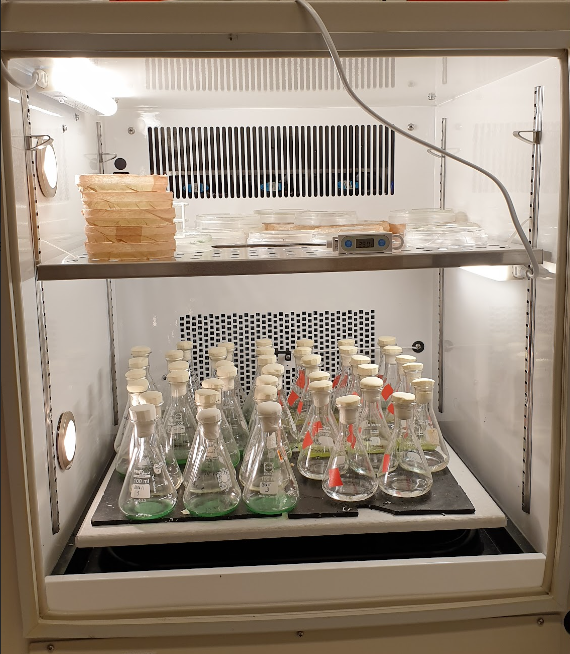
\includegraphics[width=0.7\textwidth]{images/chap2/chap2_cyano_02.png}
    \label{fig:ch2cyano02}
    \caption{Growth curve of Cyanobacteria in different conditions. Optical density at a wavelength of 544 nm was measured every 24 hours. Conditions are as followed BG11 (standard medium), BG11 with different pHs (6,7,8), BG11 with different salt conditions (Brackish, Sea Water) and water collected from the Baltic Sea and the West Coast of Sweden (Gotland, Göteborg). Data is presented ± SEM} 
\end{figure}
\FloatBarrier

\epigraph{The following section was written by members of the Sorbonne team}{\textit{iGEM Sorbonne\_U\_Paris 2021}}
\subsection{Algae}
The "algae" are a polyphyletic group of eukaryotic organisms capable of photosynthesis. Until very recently, the classification of algae was based only on morphological criteria, so that these organisms can be found in many groups of protists, such as Euglenozoa, Stramenopiles or Dinoflagellates. As a result, this group has an incredible phenotypic and genetic diversity, which can be a challenge for their culture as well as an advantage for their isolation. We will focus here on unicellular algae, on which most of the synthetic biology work is currently concentrated, and we will discuss culture and isolation methods for both environmental organisms and reference strains available in the laboratory.
\begin{figure}[!htbp]
    \centering
    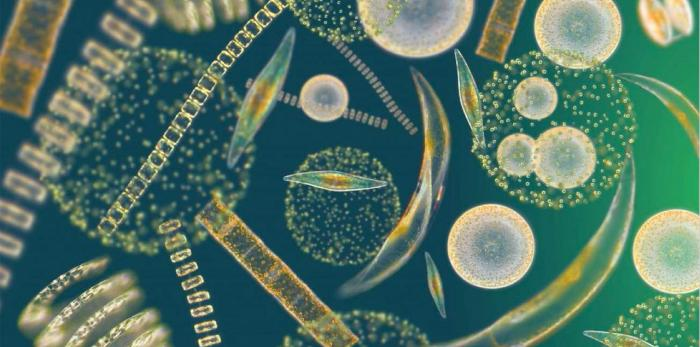
\includegraphics[width=\textwidth]{images/chap2/chap2_alg_01.png}
    \label{fig:ch2alg01}
    \caption{Marine and lacustrine algae do not constitute a homogeneous monophyletic group: as a result, they possess an incredible diversity of forms and functions.} 
\end{figure}
\FloatBarrier
 \noindent
\subsubsection{Isolation of microalgae}
Following a sampling in the field, it may be necessary to concentrate the algae if they are in dispersed or planktonic form. This concentration step can be done by membrane filtration or by gentle centrifugation. The algae can then be quickly identified with an upright microscope before proceeding to their isolation. Several isolation methods exist, and the choice between them depends on the qualities of the targeted algae. All these methods aim at obtaining monoclonal lines.
\paragraph{Direct isolation}\mbox{}\\
Motile algae can be inseminated on an agar medium (0.5\%) with one end hidden from the light. The motile algae will then tend to move towards the light source by phototactism. The algae can thus be isolated directly under an inverted microscope using a tapered Pasteur pipette before being transferred to sterile medium. An alternative is to use an atomizer which sprays water droplets containing isolated algae on the culture medium. Once the colonies are formed, it is then possible to transfer them on sterile medium.
\paragraph{Selective enrichment}\mbox{}\\
Selective enrichment consists in growing the algae in a medium that only allows the growth of certain target organisms and that causes the death or the stop of the growth of undesirable organisms. It is then necessary to adapt the culture media according to the qualities of the alga that we want to isolate. This method therefore requires prior knowledge of the strain that we seek to isolate. Isolation is probably done under an inverted microscope using a tapered pipette \parencite{Richmond2013}.
\paragraph{Streak method}\mbox{}\\
The streak method involves raking the culture solution onto a fairly solid petri dish (about 1\%) and then harvesting the colonies and seeding them within 96-well plates. The grown colonies can then be successively transferred to 48 and 24 wells plates before being put in flasks.
\paragraph{Density gradient centrifugation}\mbox{}\\
The use of a centrifugation gradient to separate algal species of different densities has been performed \parencite{Whitelam1983}using colloidal silica (otherwise called silica sol or Percol). This isolation allows the formation of discrete bands of algae of different density within the Persol gradient.
\paragraph{Flow cytometry and cell sorting}\mbox{}\\
Flow cytometry can also separate microalgae according to their size and pigment content. However, this method can be inaccurate and does not guarantee to obtain an axenic culture \parencite{Richmond2013}.
\subsubsection{Choice between axenic and non-axenic culture methods}
Sometimes the design of a genetic system requires the use of axenic strains. It is then necessary to eliminate all the organisms present in the coculture, whether they are protozoa, bacteria or viruses. Successive transfers on sterile medium as previously described generally allow to obtain monoclonal lines, but do not guarantee to obtain axenic lines. Several techniques can be used to obtain axenic lines. Among these, it is possible to irradiate algal cultures with UV light. Algae are generally quite resistant to UV radiation due to their production of pigments and other metabolites such as mycosporin analog amino acids \parencite{Carreto2011}. However, some bacteria are excellent extremophiles, and it is therefore important to check for the absence of opportunistic bacterial development in environments thus free of predators. Moreover, too much radiation can alter the photochemistry of the alga or induce damage to the algal genome or proteome. Therefore, antibiotics and antifungals are often used to eliminate any bacteria or fungi associated with algal cultures \parencite{Richmond2013}. However, it is observed that after several transfers to sterile media, the cultures tend to become axenic. The relevance of such axenic cultures in synthetic biology is however increasingly questioned. Indeed, several studies have shown that algae often have a set of associated bacteria in the natural environment, equivalent to the human microbiota known as the "cyanosphere". These symbiotic associations can range from the simple exchange of nutrients to the sharing of vitamins, siderophores and even antibiotics. Some articles indicate that bacterial symbionts of \textit{Chlamydomonas reinhardtii} such as \textit{Leisfonia sp.} would increase biohydrogen production by the alga or that different species of pseudomonas associated with Chlorella vulgaris would allow for more biodiesel production \parencite{Yao2018}. The study of symbionts in "domesticated" algae could therefore be crucial in large-scale production perspectives or in the simple maintenance of algal cultures over time. Some algal libraries, such as that of the Muséum National d'Histoire Naturelle in Paris, have already opted for non-axenic cultures, which are less demanding and more sustainable over time.

\begin{figure}[!htbp]
    \centering
    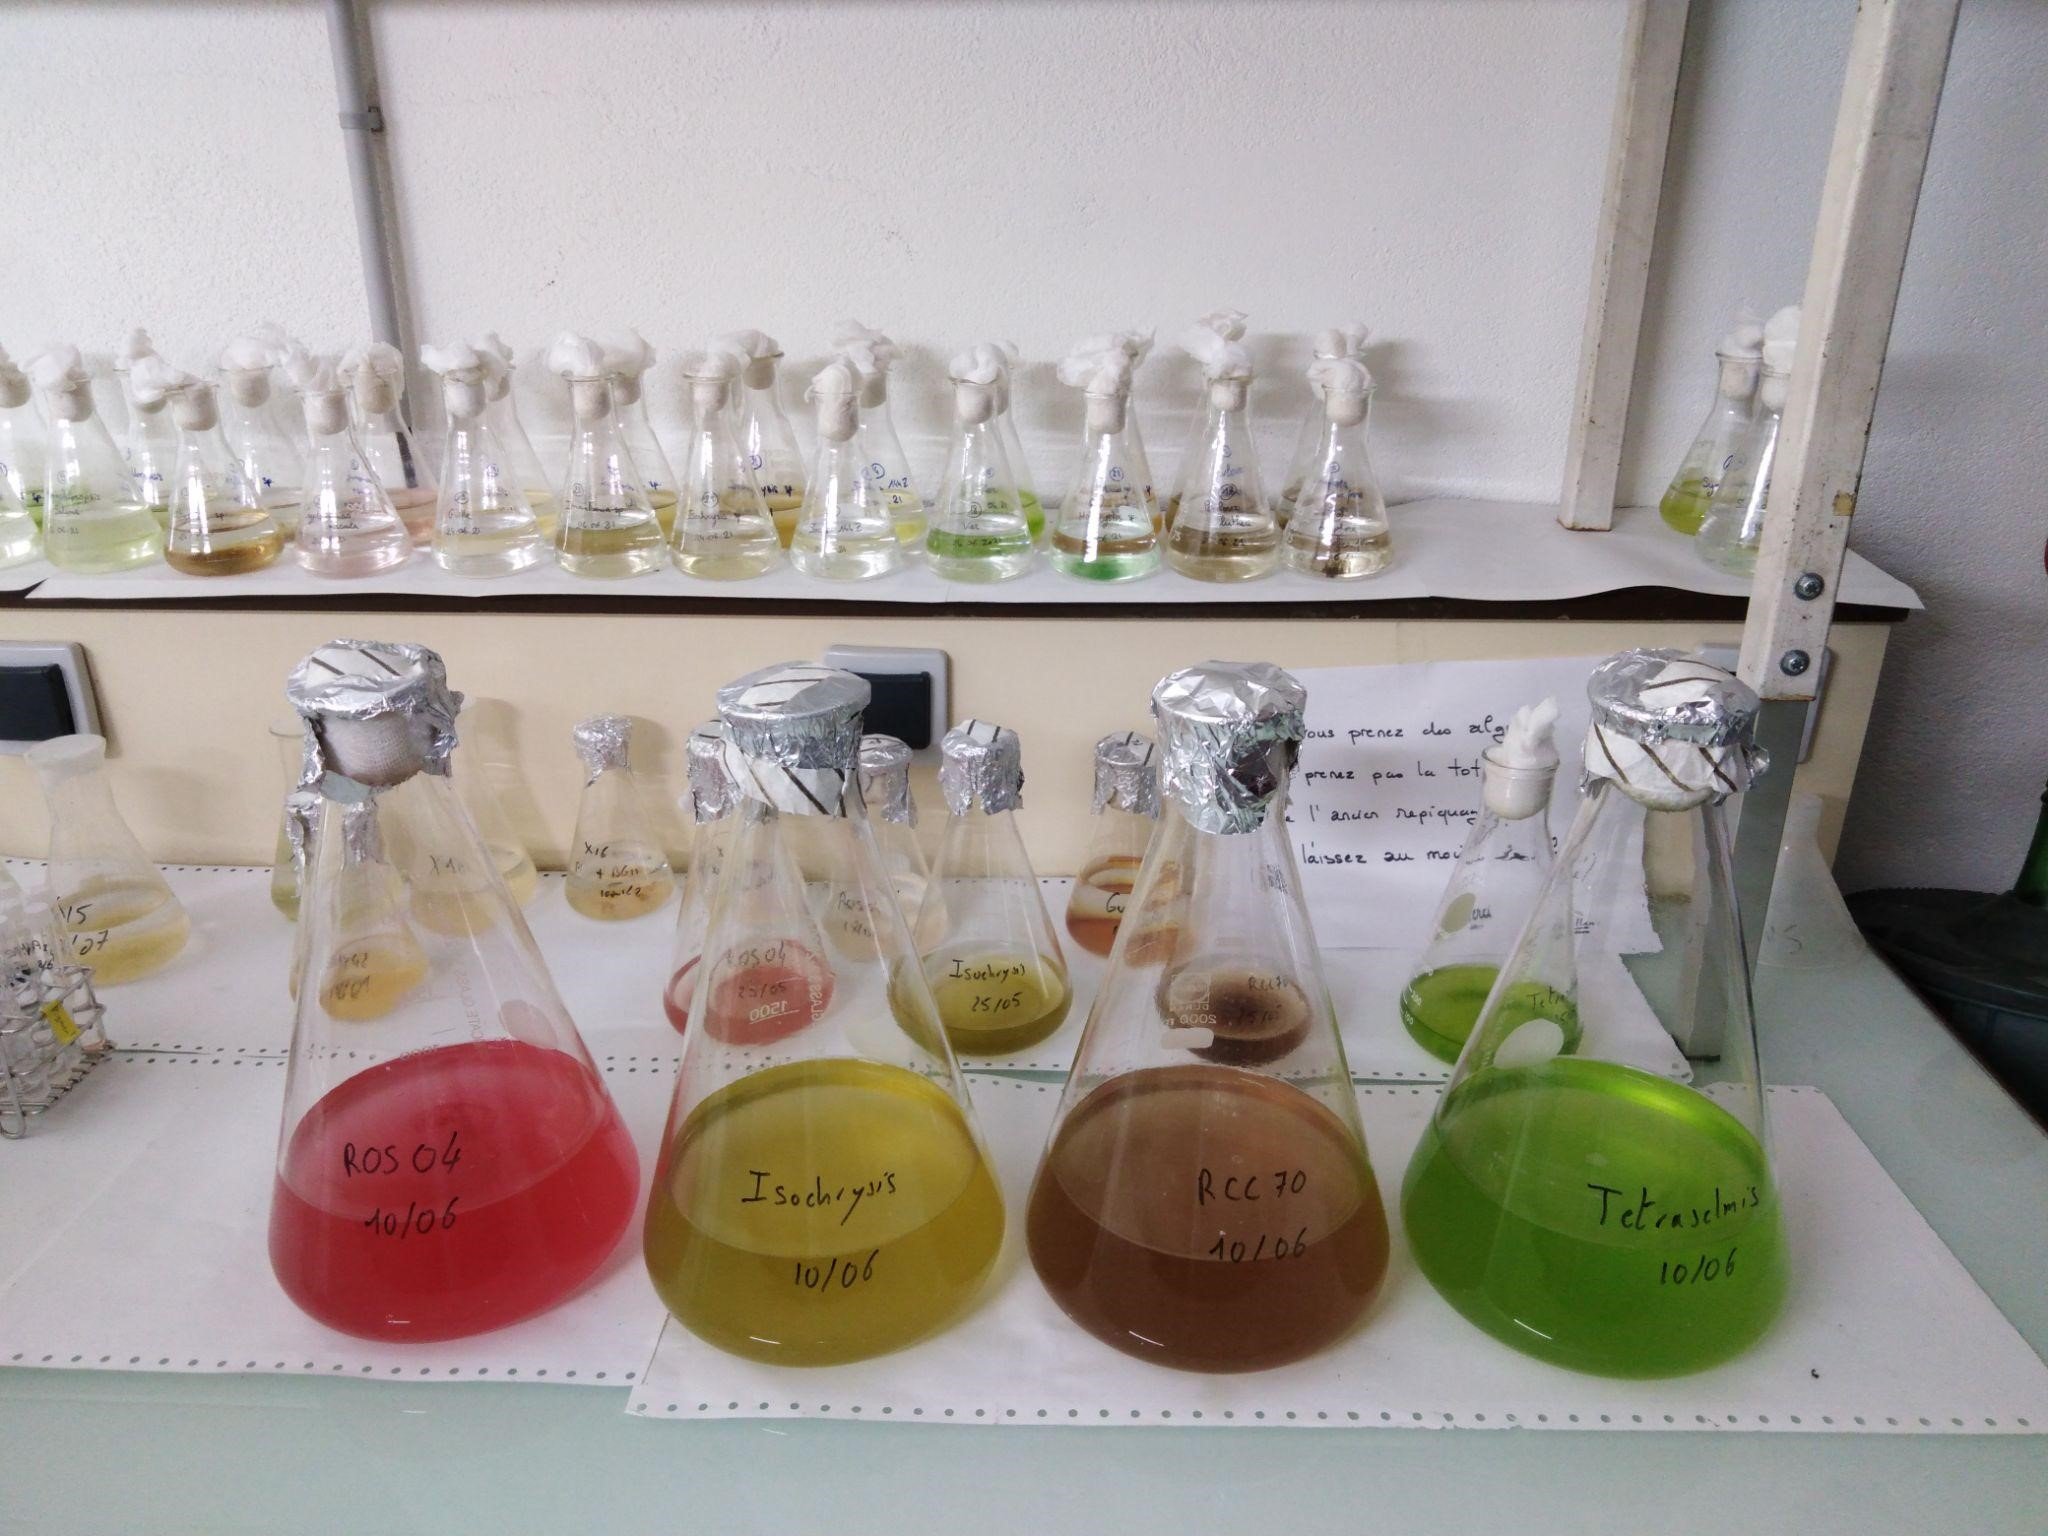
\includegraphics[width=\textwidth]{images/chap2/chap2_alg_02.jpg}
    \caption{Several algal libraries, such as the one at the marine ecology station of Banyuls-sur-Mer (Sorbonne University, France), have adopted a non-axenic culture method that is closer to the conditions of culture in natural environments.}
    \label{fig:ch2alg02}
\end{figure}
\noindent
\subsubsection{Maintenance of algal cultures for strain conservation}
Once the monoclonal cultures are obtained, it is possible to place them in flasks with a cap allowing gas exchanges. The cultures can then be placed in incubators, where the humidity, light and temperature are regulated according to the algae and the desired objective: multiplication of the algae or simple maintenance in the culture medium. For cultures with a large number of different algae, mainly from temperate or warm regions, it is possible to set at 25°C \parencite{Georgianna2012}. Transplanting will then need to be scheduled on a regular basis (usually every two months but to be estimated based on the growth of the algae). Species from temperate regions can be placed at lower temperatures (between 18 and 19°C) to reduce transplanting time, but a higher temperature will still be required for strains from tropical regions. White light lamps or natural light should be favored, in order to give the algae the widest possible spectrum and to have a larger collection, but it is still possible to select certain wavelengths to favor the growth of certain organisms, following research in the literature to verify the absorption spectra of the pigments. The new LED lights have the advantage of being easily positionable and adjustable to the needs of the algae, but a natural light can bring environmental variations whose benefit over time is not to be neglected. Thus, some laboratory scientists report empirically that unchanging environmental conditions (composition of the medium, temperature...) tend to weaken the algal cultures of collections over time, although optimal conditions are favored for mass production, so that experimenters tend more and more to reproduce the natural environment of algae. For simple conservation, the algae can be stored without any agitation in the culture chamber or incubator, but for mass production as often desired in molecular biology, regular agitation on an orbital shaker tray is preferred.
\subsubsection{Main culture media for model organisms in synthetic biology}
In this section, we will mention the main culture media for model algal organisms in synthetic biology.  It should be noted that depending on the metabolic activity targeted during the experiments, it is sometimes necessary to adapt the culture conditions of each alga.
- \textit{Chlamydomonas reinhardtii}: This is one of the algae for which a MoClo Toolkit has been defined \parencite{Crozet2018}, and is therefore one of the most widely used algae in synthetic biology. \textit{Chlamydomonas reinhardtii} has the advantage of being a mixotrophic alga, so it can be grown in heterotrophic media to accelerate yields. The TAP medium (TRIS acetate phosphate) remains the reference medium for the different strains, but the presence of acetate tends to decrease the photosynthetic activity of the alga, it is recommended to use a minimum medium if this activity is part of the parameters to be tested during the experiment. Thus, the HSM medium is used as reference medium for the study of autotrophy in \textit{Chlamydomonas reinhardtii}. Several authors recommend to supplement the TAP medium with different compounds such as phytohormones or antibiotics.

\begin{figure}[!htbp]
\floatbox[{\capbeside\thisfloatsetup{capbesideposition={left,top},capbesidewidth=6cm}}]{figure}[\FBwidth]
{\caption{Cultures of Chlamydomonas reinhardtii. It is possible to monitor the growth of the algae in a very visual way: the greener the culture appears the more concentrated the algae is. Thus, the first Erlenmeyer flask on the left does not contain a sufficient concentration of algae to proceed to a transformation, while those on the right seem to be sufficiently concentrated. More opaque green cultures are usually too concentrated and should be diluted. The medium should appear homogeneous under agitation, otherwise the culture may be contaminated.}
\label{fig:ch2alg03}}
{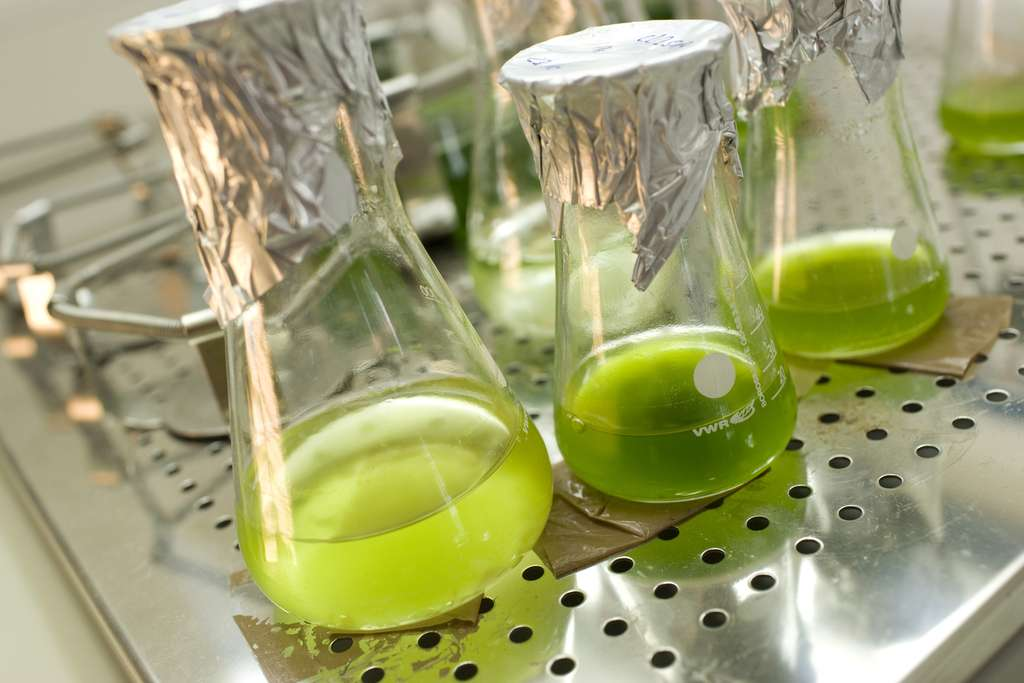
\includegraphics[width=8cm]{images/chap2/chap2_alg_03.png}}
\end{figure}
\FloatBarrier
\noindent
\paragraph{Other informations about the culture of \textit{Chlamydomonas reinhardtii}} \mbox{}\\
The generation time of the cells is 8 hours and the exponential phase is 1 to 5 million cells per mL. Care should be taken to ensure that the cell concentration remains stable during the experiment. The cells are agitated during the whole culture.
Protocol TAP medium: \href{https://www.protocols.io/view/TRIS-acetate-phosphate-TAP-medium-e95bh86}{www.protocols.io}.
Protocol HSM medium : \href{https://www.protocols.io/view/Sueoka-s-High-Salt-Medium-fdebi3e}{www.protocols.io}

\begin{description}
\item[\textit{Ostreococcus tauri}]\mbox{}\\ 
Ostreococcus tauri is the smallest eukaryotic photosynthetic organism known at present \parencite{Chretiennot-Dinet1995}. It is a marine microalga discovered in the 1990s in the Etang de Thau, in the French Eastern Pyrenees. The genome of O. tauri is very short, about 12,513 bp \parencite{Derelle2006}, and has sometimes been cited for synthetic biology studies, mostly for basic research purposes. The algae are grown in ASW (Artificial Sea Water, see composition at \href{https://www-cyanosite.bio.purdue.edu/media/table/asw.html}{www-cyanosite.bio.purdue.edu}) medium within an incubator under a light intensity of about 20 µmol.m-2.s-1 placed at 20°C \parencite{vanOoijen2012}. The cells do not have to be agitated during culture, but the handler must ensure that the algae are resuspended daily.
 
\item[\textit{Phaeodactylum tricornutum}]\mbox{}\\
The diatom \textit{Phaeodactylum tricornutum} represents one of the main hopes of synthetic biology since TALEN endonucleases and the Cas9 system were used to modify its genome \parencite{Kroth2018}. \textit{Phaeodactylum} cultures are placed under agitation (120 rpm), at a temperature of 22°C and an irradiance of 152 µEinstein.m-2.s-1. The composition of the algal culture medium is given within the article by \parencite{Bitaub2008} available at \href{https://www.sciencedirect.com/science/article/pii/S1369703X08000648}{https://www.sciencedirect.com/science/article/pii/S1369703X08000648}
 
\item[\textit{Thalassiosira pseudonana}] \mbox{}\\
This is another model diatom in synthetic biology for which the Golden Gate cloning method is applicable, but for which there is not yet a MoClo toolkit \parencite{Kroth2018}. Cells are placed at 20°C with agitation in ASW medium (see \textit{Ostrococcus tauri}) supplemented with 1 µg.L-1 vitamin B12 \parencite{Cook2015}.
 
 \begin{figure}[!htbp]
\floatbox[{\capbeside\thisfloatsetup{capbesideposition={right,top},capbesidewidth=6cm}}]{figure}[\FBwidth]
{\caption{The diatom \textit{Thalassiosira pseudonana} (above with its two silica frustules) represents one of the main hopes of synthetic biology, although no MoClo toolkit has yet been created for it.}
\label{fig:ch2alg04}}
{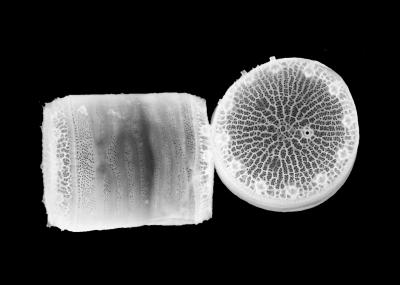
\includegraphics[width=8cm]{images/chap2/chap2_alg_04.png}}
\end{figure}
\FloatBarrier
 \noindent
\item[\textit{Dunaliella salina}] \mbox{}\\ 
Dunaliella is known to be one of the major commercial sources of β-carotene, but its significant production of lipids, proteins, and vitamins makes it likely to become a synthetic biology model in its own right in the future. The pigment color of the cell depends on the salinity of its environment: Dunaliella turns red when exposed to salinities above 25\% because it then loads up with carotenoids. Dunaliella salina is only autotrophic, the quality of the light to which it is exposed is thus very important, this light must be natural or white. Its optimum temperature is between 25 and 35°C and its optimum pH between 9 and 11. This alga requires a continuous supply of CO2, either in the form of gas or 10 mmol.L-1 of NaHCO3 \parencite{Hosseini2009}. The optimal culture medium for obtaining β-carotene is described in the article by \parencite{Morowvat2016} available at \href{https://www.sciencedirect.com/science/article/pii/S1878818116301773?via\%3Dihub}{https://www.sciencedirect.com/science/article/pii/S1878818116301773?via\%3Dihub}.

 \begin{figure}[!htbp]
\floatbox[{\capbeside\thisfloatsetup{capbesideposition={left,top},capbesidewidth=6cm}}]{figure}[\FBwidth]
{\caption{\textit{Dunaliella salina} changes color according to the salinity of the environment}
\label{fig:ch2alg05}}
{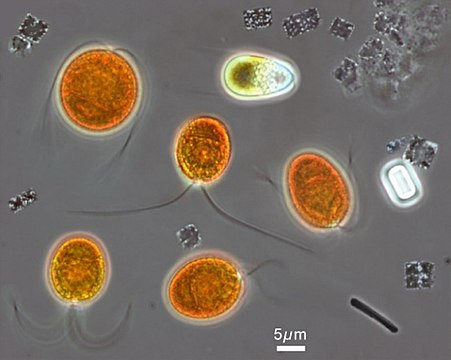
\includegraphics[width=8cm]{images/chap2/chap2_alg_05.png}}
\end{figure}
\FloatBarrier
\end{description}



% =====================================================================
% ============================== CHAPTER ==============================
% =====================================================================

\chapter{Transformation}

\section{Cyanobacteria}
\epigraph{The following sections were written by Malin Eriksson and Maxence Holtz}{\textit{iGEM Aboa \& Toulouse\_INSA-UPS 2021}}
\subsection{Overview}
The ability to transform an organism is essential in any synthetic biology project. Exogenous DNA can be introduced into cyanobacteria mainly in three different ways, either for the chromosomic integration of transgene expression cassettes through homologous recombination or for the transfer of stably replicable plasmids. These approaches are natural transformation, electroporation, and conjugation. The method of choice depends on many factors, including cyanobacterial strain and available equipment.

\subsection{Natural transformation}
Many cyanobacterial species are naturally competent, meaning that they readily take up exogenous DNA from their environment . Cyanobacteria can integrate the exogenous DNA into their genome through homologous recombination or maintain circular heterologous DNA elements in the presence of a proper replication origin. Natural competency has not been studied in as much detail in cyanobacteria as it has in many heterotrophic organisms \parencite{Schirmacher2020}. Thus, many aspects relating to the exact mechanism of DNA uptake are still somewhat unclear. The two most discussed hypotheses for the advantages of natural competence are DNA-for-diversity and DNA-for-food. The DNA-for-diversity hypothesis suggests that the benefit of natural competence is the ability to obtain new features, whereas the DNA-for-food hypothesis states that DNA uptake is nutriciously important \parencite{Schirmacher2020}. \\ \\
Naturally competent cyanobacteria provide an efficient and easy-to-use method for the introduction of foreign DNA into the cells. In brief, this transformation method only requires the DNA that is to be taken up and a cyanobacterial liquid culture to which it will be mixed into. Thus, no particular equipment or reagents are necessary besides those found in a cyanobacteria culture laboratory and preparation time is minimal. Protocols for natural transformation tend to vary between research groups, and also may need some adaptations from one species to another, meaning that no consensus has been reached. Optimization attempts have usually circled around changing parameters such as incubation time, light conditions during incubation, DNA concentration, cyanobacterial growth phase, and plating style \parencite{Zhang2007}. \\ \\
Relying on the natural competence of cyanobacteria is, however, not always possible, as only certain cyanobacterial strains carry this trait. Cyanobacteria within the \textit{Synechocystis} and some within the  \textit{Synechococcus} genus are naturally competent \parencite{Schirmacher2020}. These are among the most well-studied and used cyanobacteria in research, but if the project plan involves utilization of other species, another transformation method could be vital. It is important to emphasize that certain species, such as spirulina (\textit{Arthrospira platensis}) that is widely used as a nutritional protein source, have not been successfully transformed to date. 

\subsection{Conjugation}
Conjugal transfer of DNA between bacterial cells is a well-described process and has been used previously to engineer cyanobacterial species, particularly those that are not naturally competent, such as \textit{S. elongatus} UTEX 2973 \parencite{Elhai1988} \parencite{Yu2015}. To obtain stable conjugal transfer it is necessary (1) conjugal contacts to be made, (2) the transferred DNA to escape restriction or degradation, and (3) the transferred DNA to replicate autonomously or integrate into one of the replicons of the recipient \parencite{Elhai1988} \parencite{Gale2019}. \\ \\
In brief, cyanobacterial cultures are incubated in the presence of two different E. coli strains called respectively the conjugal strain and the helper strain. Note that in some variations of this protocol, only one E. coli strain carries all the plasmids. The helper strain carries two plasmids: the vector to be transferred to the cyanobacteria called cargo vector and a helper plasmid. The latter encodes for specific DNA-methylases that act on the cargo vector so that it is not degraded after entry into the cyanobacterium cellular space (step (1) of Figure 3.1). The conjugal plasmid carried by the conjugal strain contains the many genes required to encode the conjugal apparatus. In the first step of conjugation, the conjugal plasmid is transferred from the conjugal strain to the helper strain (step (2) of Figure 3.1). This helper strain is then able to transfer the methylated cargo vector into the cyanobacterium (step (3) of Figure 3.1). For this process to work, the cargo vector must be compatible with the conjugation system (i.e. it must contain an appropriate origin of transfer (oriT), also known as a bom (mobility base) site) \parencite{Elhai1988} \parencite{Gale2019}. Additionally, special attention must be paid to use compatible conjugal, helper and cargo plasmids in E. coli : the origins of replication on these three plasmids must not belong to the same incompatibility group and the antibiotic resistance must not overlap.

\begin{figure}[!htbp]
    \centering
    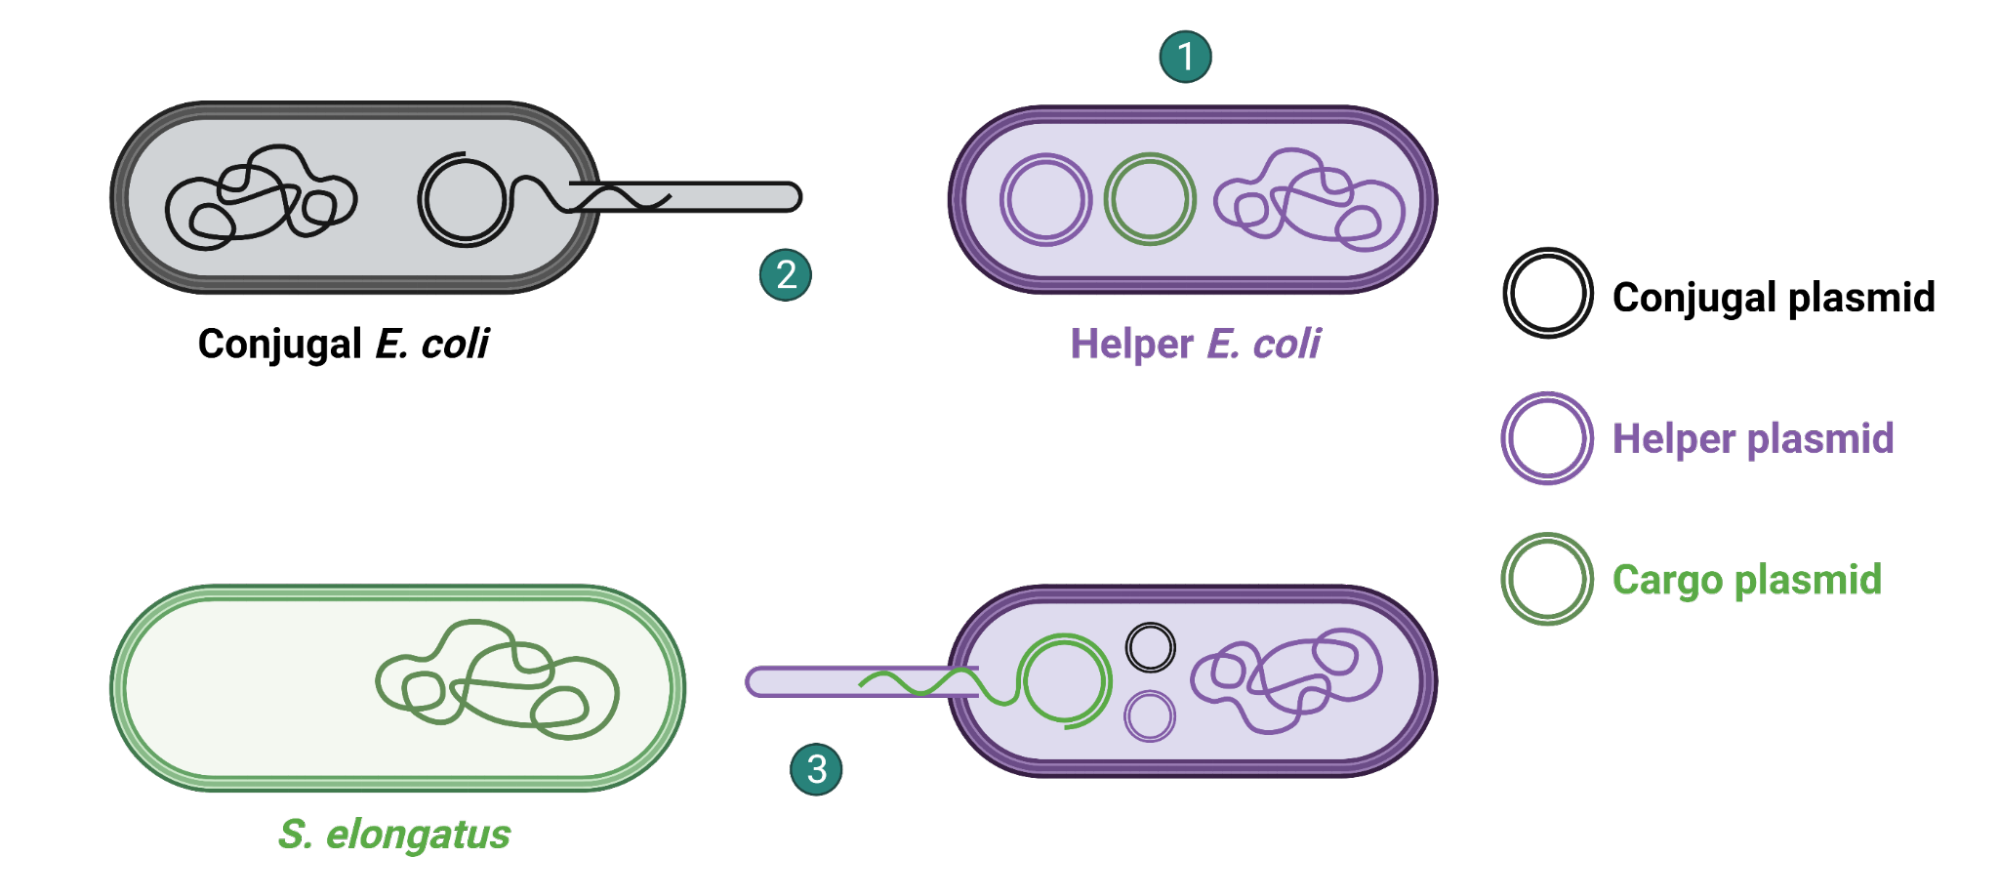
\includegraphics[width=\textwidth]{images/chap3/cyano/image1.png}
    \label{fig:ch3cyano01}
    \caption{Transfer of DNA into a cyanobacterium (green) through triparental mating (iGEM Toulouse 2021).} 
\end{figure}
\FloatBarrier

\noindent
There are several different conjugal and helper plasmids available, the most widely used in cyanobacterial research being respectively pRL443 (\href{https://www.addgene.org/70261/}{https://www.addgene.org/70261/}) and pRL623 (\href{https://www.addgene.org/58494/}{https://www.addgene.org/58494/}). The E. coli HB101 strain is furthermore frequently used for this type of protocol. More information on the practical protocol details can be found in the well-illustrated video article provided by \parencite{Gale2019}.
Overall, although theoretically the triparental mating process may seem complicated, in practice it is quite easy to perform and provides satisfactory transformation efficiencies for most applications. This technique is widely applied for species and strains that are not naturally competent. In some instances, conjugation may furthermore be the preferred route of DNA transfer, particularly when a large segment of foreign DNA is to be transferred or if merodiploids (single recombination events) are desired \parencite{Yu2015}. Note that certain species are refractory to conjugation, maybe due to thick cell walls or strong endonuclease activities.



\subsection{Electroporation}

Electroporation is the process of transferring DNA into bacteria or other cells by momentarily opening the pores of cell membranes with a pulse of electricity. A few species of cyanobacteria have been shown to be transformable by electroporation in laboratory conditions \parencite{Koksharova2002} \parencite{Stucken2012} \parencite{Tsujimoto2015}. \\ \\
If the strain of interest is not naturally competent and conjugation is impossible (some cyanobacteria - specific genetic sequences are toxic to E. coli), this method may be of interest \parencite{Wendt2019}. \\ \\
Nonetheless, in cyanobacteria, electroporation transformation has limitations. Earlier research has revealed that electroporation is inefficient and requires a considerable amount of donor DNA \parencite{Toyomizu2001}. Furthermore, the extracellular polysaccharide layers found in some cyanobacteria species cells act as physical barriers to DNA entering the cell \parencite{Wendt2019}. Moreover, electroporation may generate double strand DNA breaks within the cyanobacterial host genome and induce some undesired mutations.





\section{Higher Plants}
\epigraph{The following sections were written by Julia Macholl}{\textit{iGEM Bielefeld-CeBiTec 2021}}
\subsection{Overview}
There are many different techniques to transform plant or plant tissues that can be mainly separated into two big categories: Plants can be either transformed directly or indirectly, meaning that either the plant or plant tissue is directly transformed by physical or chemical methods or indirectly by using a biological host for the gene transfer. Many laboratories use either agrobacterium mediated transformation or particle bombardment due to practicality, simplicity, and efficiency \parencite{Keshavareddy2018}. 


\subsection{Indirect Methods}
The most common indirect method to transform plants or single plant cells is agrobacterium-mediated transformation \parencite{Hwang2017}. The soil bacterium \textit{Agrobacterium tumefaciens} has the natural ability to transform many dicot and monocot angiosperm as well as gymnosperm plants by incorporating T-DNA into the host genome \parencite{Gelwin2003}. For that, it carries a tumor inducing (Ti) plasmid that contains the T-DNA and vir genes that are, besides others, necessary to integrate the T-DNA into the plant genome. To transform plants, a binary vector system is used. The first vector contains the gene of interest that is flanked by T-DNA borders so that it will be incorporated into the plant genome. It also contains other important features like selection markers and origins of replication. The second vector – the Ti-helper plasmid – is carrying the vir-genes \parencite{Lee2008}.
\\

\begin{figure}[!htbp]
    \centering
    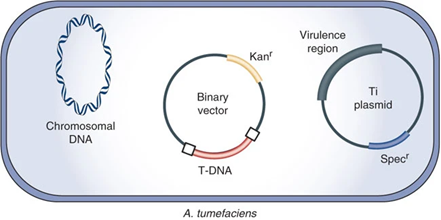
\includegraphics[width=\textwidth]{images/chap3/higher plants/image1.png}
    \label{fig:ch3high01}
    \caption{\textit{Agrobacterium tumefaciens} containing its chromosomal DNA, the Ti-helper plasmid and the binary vector \parencite{Michielse2008}.} 
\end{figure}
\FloatBarrier

\noindent
Transformation targets can either be tissue cultures or whole plants. (Stable transformation can be achieved with tissue cultures or whole plants.) For tissue cultures, plant cells are co-cultivated with agrobacteria for transformation \parencite{Keshavareddy2018}. Then, cells are cultured on media for formation of calli, which are unorganized plant cell mass. Calli can also be grown to whole transgenic plants in the end, which takes quite a long time.
Whole plants can also be transformed by several methods that were developed over time. One of the earliest methods developed was transformation by vacuum infiltration which can be performed not only on \textit{Arabidopsis} \parencite{Clough1998}, but also on other plants like Brassica campestris or Raphanus sativus. However, this method is quite labor intensive \parencite{Keshavareddy2018}. That is why it was replaced by more efficient techniques like floral dipping, where the flowers are dipped into agrobacterium suspension or floral spraying, where the agrobacterium suspension is sprayed onto the flowers. The advantage of in planta transformation in comparison to cell tissue transformation is that the gene of interest can be directly transferred into reproductive plants \parencite{Keshavareddy2018}.
\\
Besides stable transformation, transient expression of genes is also possible. The most prominent example is agroinfiltration with \textit{Nicotiana benthamiana}. For that, agrobacteria are injected into the underside of the leaf when the tobacco plants are ideally 4-6 weeks old. Two days after infiltration, the gene of interest should be expressed and experiments can be performed. Agroinfiltration is an easy method for screening constructs very quickly \parencite{Bally2018}. In comparison to stable transformation, which can take months or even up to years, transient expression with agroinfiltration allows quick screening in just a few days. 

\begin{figure}[!htbp]
    \centering
    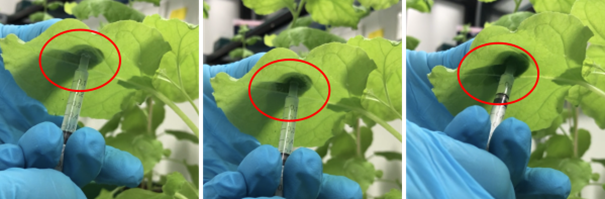
\includegraphics[width=\textwidth]{images/chap3/higher plants/image2.png}
    \label{fig:ch3high02}
    \caption{\textit{Agrobacterium} suspension is injected into the leaf with a needleless syringe.} 
\end{figure}
\FloatBarrier



\subsection{Direct Methods}
\epigraph{The following section was written by Jessica Baumann}{\textit{iGEM 
Marburg 2021}}
\noindent
Besides the indirect methods of transforming higher plants, there is also the direct method of biolistic bombardment. Biolistic bombardment is a process in which a gene construct is fired into plant cells using a particle gun. In this process, DNA is coupled to either gold or tungsten particles and is then catapulted into selected leaves under high pressure. 
This introduces the inserted DNA into the DNA of the chloroplast by homologous recombination. After successful insertion of the DNA, selection by antibiotics occurs, allowing only the transgenic plant cells to regenerate. First, it is important that the plants used for transformation grow sterile. For this purpose, at the beginning the seeds of the selected plants are sterilized by bleach and hydrochloric acid, and are then transferred to plant regeneration medium in deep petri dishes, where they begin to germinate. When the plantlets have reached a size of 1 cm, they are transferred to new petri dishes, where they continue to grow in fresh Plant regeneration medium. After a further growth phase, the plants are transferred to magenta boxes containing plant maintenance medium. The plants are grown in the magenta boxes until they reach a size of ~10 cm. Once the plants have reached this height, the biolistic bombardment can begin. 
\\ \\
For this purpose, the gold or tungsten particles are first prepared by repeatedly washing them with ethanol in several steps. For this purpose, the gold or tungsten particles are first prepared by repeatedly washing them with ethanol in several steps. To coat the Dna onto the particles, it is added to the particles while they are shaken on the vortex. After several more rounds of centrifugation, the particles are ready for the bombardment. First, however, the individual leaves of the sterile plants must be prepared for bombardment. For this purpose, 2 Whatman filter papers are applied to petridishes containing RMOP medium. The leaves previously harvested from the plantlets are placed centrally on the filters. It is important to sterilize the inner surfaces of the particle gun, as well as all other objects to be used, such as rupture disks or macrocarriers, etc., with ethanol. The DNA-coated particles are pipetted onto the macrocarriers. All individual components of the particle gun are assembled and the plates containing the sheets to be coated are placed one by one under the microcarrier launch assembly. Due to the pressure caused by the helium, the gold particles are bombarded into the plant cells. The bombarded plates are closed and sealed with micropore tape. Leaves are incubated in the Petri dishes for 2 days in a Culture room before leaf samples are transferred to additional plates containing a specific antibiotic. Several laef samples with a size of 1cm\textsuperscript{2} are cut out and transferred onto the antibiotic plates. These plates are also sealed with Micropore tape and again placed in the culture room. 6 to 12 weeks the leaf samples are kept on the medium until green calli or shoots are then formed. When spectomycin is used as an antibiotic, it can also happen that a spontaneous mutation in the 16S rRNA leads to resistance to the spectomycin just named. It remains to be determined which cells are truly transplastomic. If spectomycin is used for selection, small sections of calli or leaves are transferred to plates containing nict only spectinomycin but also streptomycin. The spontaneous mutation only introduces resistance to spectinomycin, but not to streptomycin. Thus, only transplastome cells remain. Whether the transgenes have really been inserted still has to be tested by PCR and DNA gel blot analysis. Rerun the plant regeneration on the selective RMOP medium and.
Validate the consistent transformation of the ptDNA by gel blot analysis. The transformed plants are then planted in soil and remain there until seeds are formed. These are collected and germinated again on antibiotic-containing plant maintenance medium. The transformed seedlings will appear dark green. 




\begin{figure}[!htbp]
    \centering
    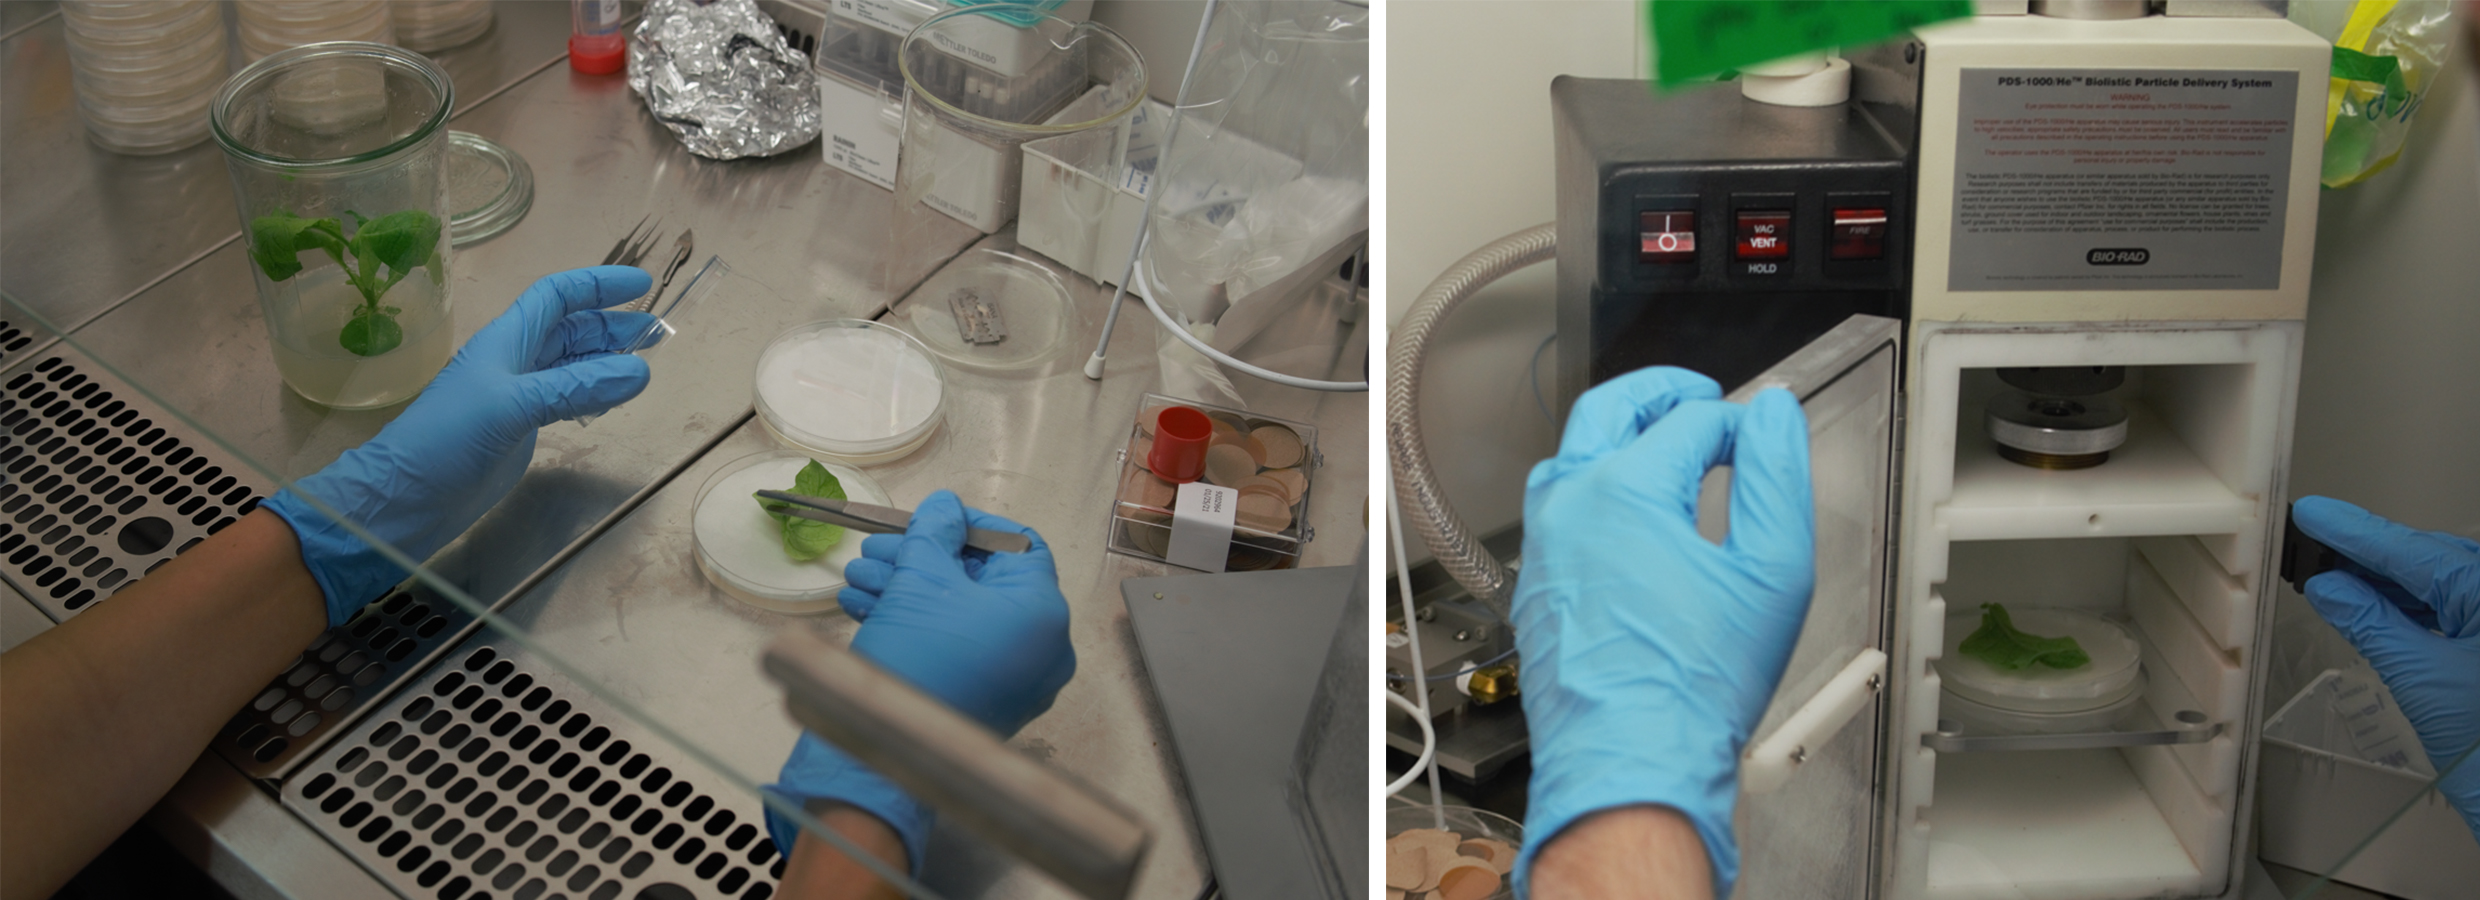
\includegraphics[width=\textwidth]{images/chap3/higher plants/image5.jpg}
    \label{fig:ch3high05}
    \caption{(a) Transfer of \textit{Nicotiana tabacum} leaves before bombardment with the gene gun. (b) The same leaf in the gene gun directly before introduction of a transgene.} 
\end{figure}
\FloatBarrier

\pagebreak

\section{Algae}
\epigraph{The following sections were written by members of the Sorbonne team}{\textit{iGEM Sorbonne\_U\_Paris 2021}}

\subsection{Overview}

The introduction of DNA into an organism allows the creation of de novo functions. This foreign DNA carry genes that usually code for a protein that provides this new function or a protein that is an intermediary to a compound that provides this function. Many of the epitomes of biotechnology are based on this principle. One notable example is the Golden rice, a rice variety that expresses components of the Β carotene pathway. This rice was engineered to improve the levels of vitamin A precursor to combat malnutrition worldwide.
\\ \\
The introduction of genetic material is not as straightforward as it may sound. Algae, as other organisms, have developed strategies to degrade foreign DNA that enters their cells. They developed these strategies because humans are not the first in the history of life that try to interfere with the genetics of algae. Viruses and bacteria, but also moving genetic elements, have interfered with the genomic cellular homeostasis since shortly after the emergence of first life. In order to defend themselves, organisms form barriers in the form of membranes and cell walls and target foreign DNAs and RNAs. Furthermore, genomic instability may also lead to apoptosis. The same system may target foreign genetic material integrating into the genome. Finally, the amount of chromosomes influences the effectiveness of transferring desirable functions: diploid and tetraploid species are more resistant than species that harbour only one chromosome of each kind. 
\\ \\
To overcome these challenges, scientists have developed direct and indirect methods to introduce novel genes into cells. Direct methods rely on challenging the outer barriers, such as membranes, through mechanical, electrical, and chemical methods. Indirect methods involve the hijacking of an existing pathological system that introduces genetic material into hosts. Both know their advantages and their challenges, which we review here.

\subsection{Indirect Methods}
Changing genomes through the transformation of a different species may be an avenue to pursue in certain cases. In this approach, we employ conjugative bacteria to do the job for us. The most famous example is \textit{Agrobacterium tumefaciens} while \textit{Escherichia coli} is also capable of transforming some algae \parencite{Mosey2021}. The choice for a direct or an indirect approach firstly depends on genome that is targeted, i.e. the nuclear genome in indirect approaches. Secondly, one has to realise that one major downside of the use of conjugative bacteria is that it takes more time and requires more steps. Moreover, one will first have to successfully transform the vector, verify that transformation, coculture and invite the conjugation to occur. Only then can we start to verify the transformation and characterisation of our newly transformed algae. This process can, however, be worthwhile in difficult to access nuclear genomes or when the insert is rather large: large inserts tend to be more prone to damage by nucleases in direct cloning methods.

\subsubsection{Indirect transformation through \textit{A. tumefaciens}}
In nature, \textit{A. tumefaciens} responds to phenolic compounds in wounds of plants through the virulence genes \parencite{Gelvin2017}. These conditions have to be reproduced to efficiently transform algae with A. tumefaciens. First of all, this means that coculture of algae not only with A. tumefaciens, but also plant cells may prove advantageous. Second and most important for effective transformation is the use of a phenolic compound. This can either be acetosyringone, cinnamic acid, vanillin or coumarin \parencite{Mosey2021}. The potential of this technique in algae was demonstrated early on in \textit{Chlamydomoas reinhardtii}. Moseley and others show a comprehensive overview of the transformation of non model microalgae (Figure 3.5). Pratheesh. Vineetha, and Muraleedhara Kurup provide a comprehensive protocol for the transformation of \textit{C. reinhardtii} using agrobacterium. For a comparison between direct and indirect transformation in \textit{C. reinhardtii} find Mini and others \parencite{Pratheesh2013}.

\subsubsection{Indirect transformation through \textit{E. coli}}
Three algae species have been reported to be succesfully transformed with \textit{E. coli}: \textit{S. obliquus}, \textit{N. oleoabundans}, and \textit{P. tricornutum} \parencite{Mosey2021} \parencite{Sharma2018} \parencite{George2020} \parencite{Beratto-Ramos2018} \parencite{Karas2015}. Important factors in the success of these transformations are the time and the ratio of the algae and the bacteria.


\begin{figure}[!htbp]
    \centering
    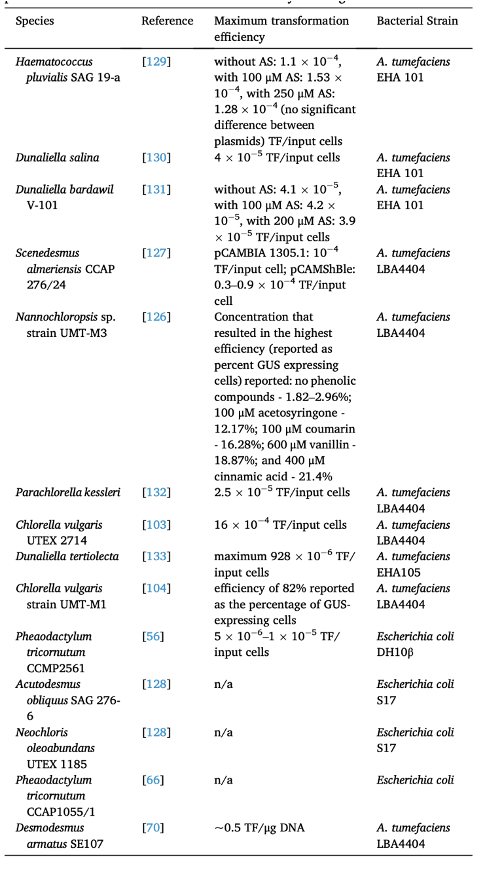
\includegraphics[width=0.8\textwidth]{images/chap3/algae/image1.png}
    \label{fig:ch3algae01}
    \caption{conditions for indirect transformations in non model microalgae \parencite{Mosey2021}.} 
\end{figure}
\FloatBarrier



\subsection{Direct Methods}
\epigraph{The following section was written by members of the Arizona State University team}{\textit{iGEM ASU 2021}}
\noindent
Our ASU iGEM 2021 team employed two direct methods of transformation into the chloroplast of the microalgae \textit{Chlamydomonas reinhardtii}. The two methods are biolistic bombardment with tungsten particles and agitation with glass beads. Most of our success this year was from our second attempt using biolistic bombardment. These two protocols were conducted under the direction of Dr. Kevin Redding, and the protocols were adapted from \parencite{Boynton1988} and \parencite{Wannathong2016} The algae used in the experiments came from the \href{https://www.chlamycollection.org/} {\textit{Chlamydomonas} Resource Center}. The sequence for the plasmid backbone used in these experiments, known as pASapI, was taken from the Wannathong paper as well \parencite{Wannathong2016}. The purpose of this section is to outline some of the tips and tricks our team learned during our time transforming the algae using these methods to help future iGEM students. The complete protocol can be found in the appendix, with some relevant notes. 


\subsubsection{Biolistic Bombardment}
Biolistic bombardment is a direct method of plasmid integration into the chloroplast. This process requires high-velocity microprojectiles made of either tungsten or gold and can utilize algae that has a cell wall (we used CC-4388). Therefore, this protocol is ideal because the resultant transformants will be easier to work with. Our experiment was conducted with 0.5 \textmu m tungsten particles in a gene gun made by Dr. Redding a few years ago (see Figure 3.6). The tungsten particles were first resuspended in glycerol, and coated in our plasmid by resuspending the DNA and the tungsten solution with calcium dichloride and spermidine. During this process, it’s important to ensure that the tungsten has not fallen out of solution and that there is never a high concentration area of spermidine, as that will lead to clumping of the tungsten/DNA. Ensure that the spermidine is added last, and the tube is being vortexed while it is added (takes practice!). Additionally, to ensure that the tungsten has not settled out of solution before placing it on the filter, the DNA solution should be sonicated thoroughly right before it is added to the filter and shot onto the plate coated in algae. This is a tedious, but important step, and make sure not to forget ear protection while sonicating! Once the filter has been loaded and screwed into the top of the chamber, ensure that the top of the agar is 11 cm from the tip of the filter. This ensures that the particle bombardment will be the correct size. The algae directly in the area of bombardment will die, and the algae near the edges of that area will survive with the plasmid integrated. Therefore, the area of bombardment should be centered on the plate, and should not occupy the whole space. In order to shoot the particles at the plate at a high enough velocity, the gene gun must create a vacuum. In our gene gun (Figure 3.6) the yellow lid sits on a rubber ring to allow the chamber to create a vacuum. Always ensure that the lid will form a complete seal before engaging the vacuum and shooting the algae. Once the bombardment has been delivered, you can see the area that was hit with the particles by holding the plate up to the light. While the rest of the agar should be clear, the area hit with the tungsten particles will appear a little hazy or fuzzy. There should not be visible dark clumps of tungsten particles. This indicates that the solution was not sonicated properly or distributed on the filter improperly. 
\\ \\
Both of these protocols utilize photosystem II deficient \textit{C. reinhardtii} and restore function of the photosystem with the plasmid. This means that photosynthesis is restored when the plasmid is integrated into the chloroplast genome. Therefore, the plates need to be stored in the light to allow for the selective selection of the transformed colonies. That being said, we initially had no success with our first round of shooting \textit{C. reinhardtii}. It was then suggested to us by our friends in Marburg that we store the algae in the dark for 24 hours before exposing it to the light. We added this step to our protocols for the second round of shooting. This time, we exposed half of the plates to the dark for 24 hours before putting them in the light and put half of the plates in the light immediately. This round of shooting was successful, but only marginally. After 4 weeks, one colony was found on three different plates, out of ~30 plates. Two of the successful plates were put directly in the light, and one of the plates was placed in the dark for 24 hours. At this point, we cannot recommend whether the light or dark protocol is more successful. 
\\ \\
Overall, we recommend a few things. First, shoot at least four different plates with the same construct. Second, ensure that the reagents used to make the tungsten/DNA solution are fresh and get mixed thoroughly. Third, double parafilm the plates before leaving them under the light to ensure no contaminants get in. Fourth, start this process EARLY. The three colonies we found were only visible one month after shooting. Finally, this process does take practice, so budget your time for multiple iterations. 

\begin{figure}[!htbp]
    \centering
    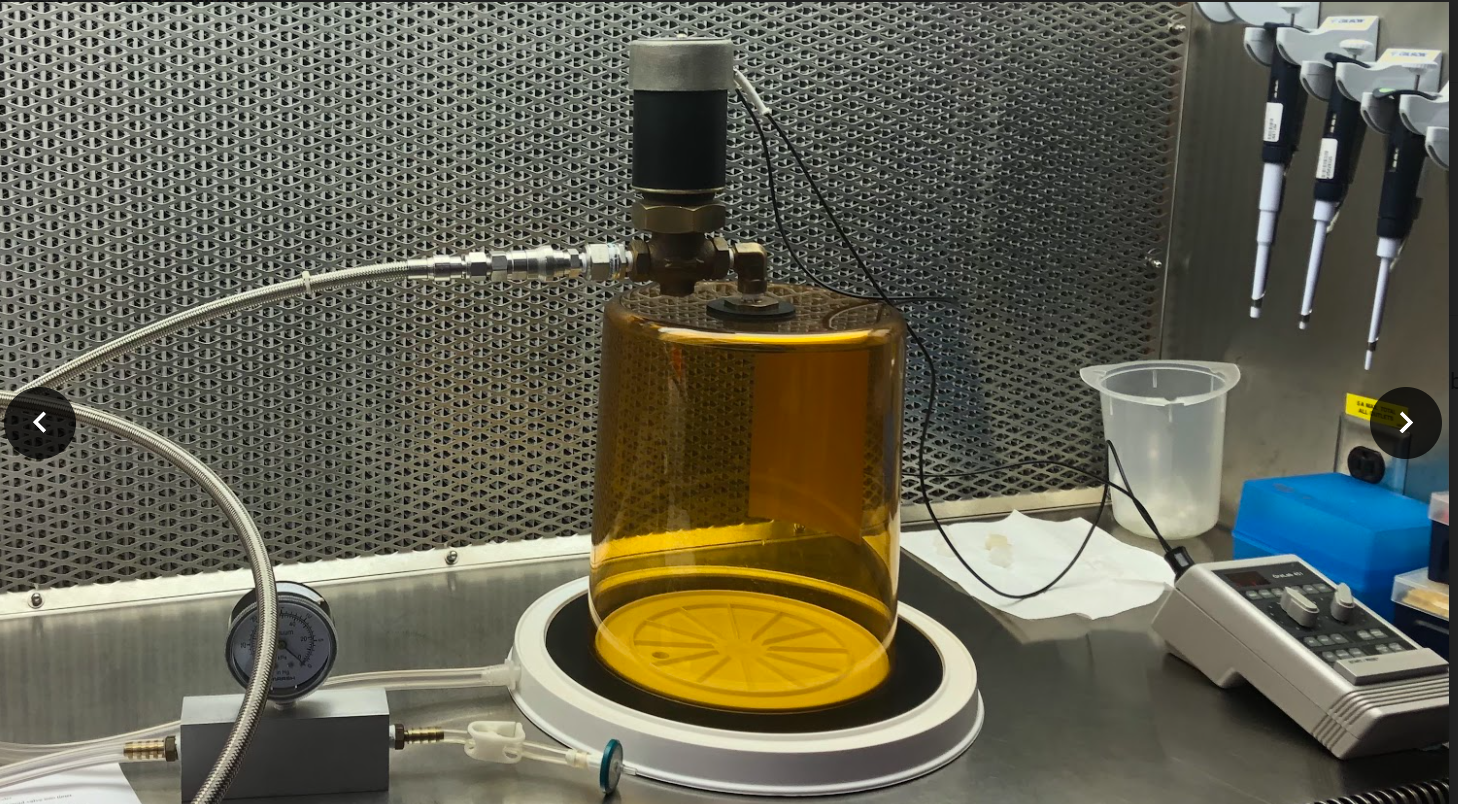
\includegraphics[width=\textwidth]{images/chap3/algae/image2.png}
    \label{fig:ch3algae02}
    \caption{The gene gun, created by Dr. Redding, set up in a laminar flow hood. On the right, the timer and button to release Helium. In the center, the yellow lid of the chamber. (Not pictured, a lab jack used to move the plate up 11 cm away from the tip of the filter).} 
\end{figure}
\FloatBarrier



\begin{figure}[!htbp]
    \centering
    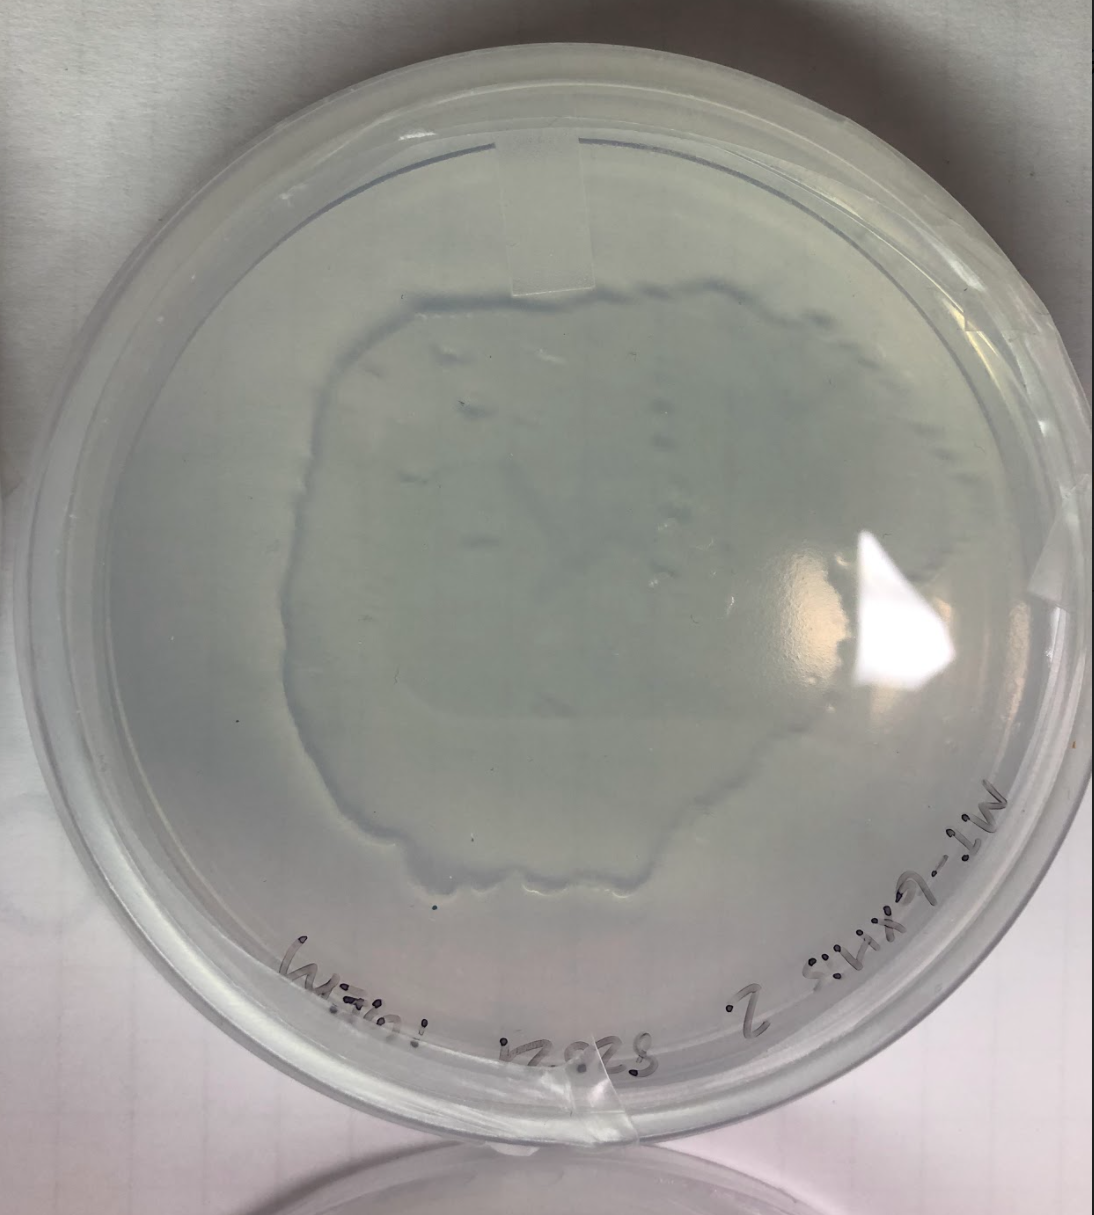
\includegraphics[width=0.7\textwidth]{images/chap3/algae/image4.png}
    \label{fig:ch3algae04}
    \caption{One of the plates with a transformed colony, creating the strain now known as iGEMC3. TBP plate, CC-4388 transformed with pASapI/MT-6xHIS. The small dark spot seen approx 0.5 cm below the “iGEM” is the successful colony. The ride that is seen at the center of the plate is water that has amassed on the lid of the plate due to condensation. It is not touching the agar of the plate and has no effect on the algae.} 
\end{figure}
\FloatBarrier




\subsubsection{Glass Bead Agitation}
Glass bead agitation is a means of integrating a plasmid into the chloroplast of \textit{C. reinhardtii}. However, this process is not ideal because it requires the use of cell wall deficient microalgae (we used CC-5168), which makes the transformant more difficult to work with. This protocol, taken from \parencite{Wannathong2016} has not yet yielded any transformants, after a full month of incubation in the light. However, it comes from a reputable source, and we had not attempted this protocol before, so it is most likely a mistake on our part. This protocol utilized cell wall and photosystem II deficient \textit{C. reinhardtii}, and the same plasmids as used in the gene gun protocol. Because our team only performed this protocol once, we do not have as many recommendations for successful transformation. 
	To make the best use of the time, it is best to aliquot out the 400-624 um diameter beads into the test tubes a day or two ahead of time, and autoclave them to ensure they are sterile. Additionally, the top agar should always be stored in a warm water bath, and should not be allowed to congeal: it should be alliquoted day of in to ~6ml samples. We plated the cells on both HSM and TBP plates, with 5\% top agar used for both plates. This protocol calls for a lot of DNA (5-10$\mu$g) in a small concentration (not more than 50$\mu$L). In order to get this concentrated DNA, we performed a miniprep on 5mL of culture and eluted the DNA thoroughly from the column. During the glass bead protocol, ensure that the vortex is at top speed, and that it runs for a full 15 seconds(Figure 3.8). Then, when removing the cells from the tube, ensure there are no glass beads clinging to the pipette tip. When mixing the cells into the top agar, invert gently and spread on the plates as evenly as possible. Ensure the top agar has congealed completely before being stored in the light. Should the colonies arise, they may be embedded in the top agar. This simply means that you’ll need to go digging for them to use the transformants. 
	Overall, we were not as successful with this protocol as we were with the gene gun. We recommend starting an assembly line of sorts with multiple lab members to work most efficiently. The algae should be removed from the glass beads, added to the top agar, and plated quickly after agitation. Additionally, the top agar should never be allowed to congeal before it is plated, and should only be removed from the warm water bath right before the algae is added. 


\begin{figure}[!htbp]
    \centering
    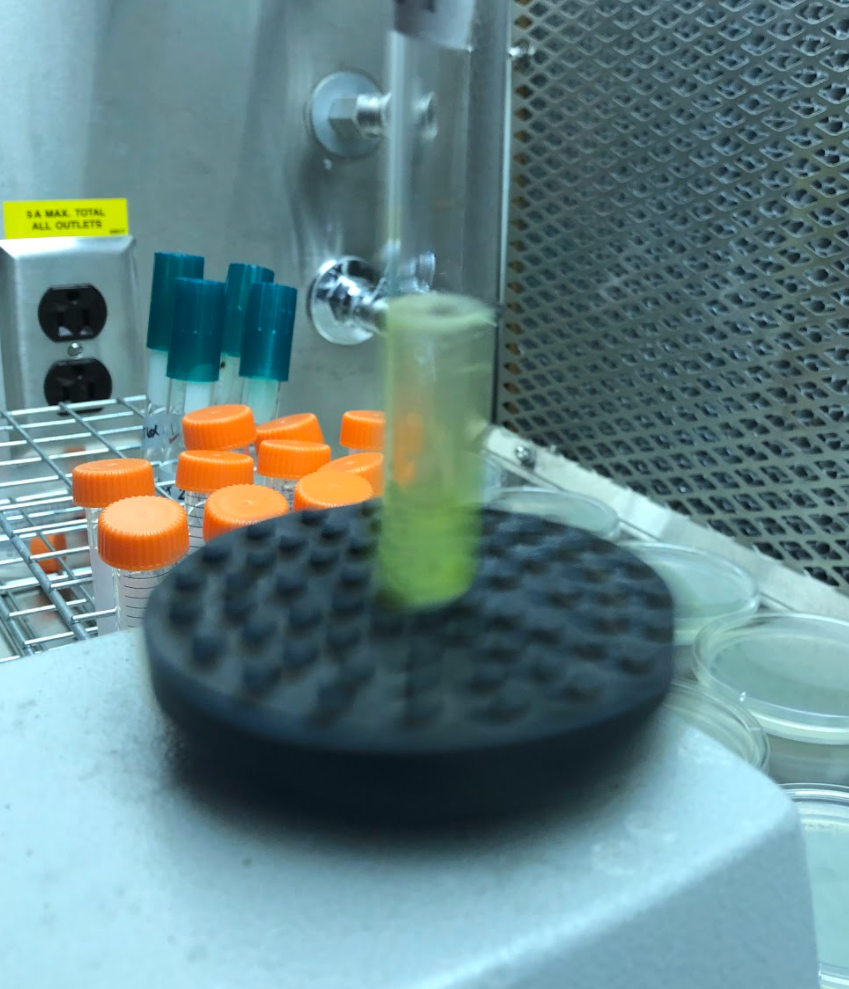
\includegraphics[width=0.8\textwidth]{images/chap3/algae/image3.png}
    \label{fig:ch3algae03}
    \caption{Test tube containing glass beads, \textit{C. reinhardtii} CC-5168, and DNA being agitated on the vortexer at max speed in the laminar flow hood.} 
\end{figure}
\FloatBarrier

% =====================================================================
% ============================== CHAPTER ==============================
% =====================================================================

\chapter{Cloning}

%\graphicspath{{images/chap4/}}


\section{Assembly Standards}
\epigraph{The following sections were written by members of the Sorbonne team}{\textit{iGEM Sorbonne\_U\_Paris 2021}}
\noindent
One of the major characteristics of synthetic biology is the ease with which we can build genetic networks. Assembly standards can be defined as the set of rules followed by the engineer to assemble bio bricks. For more than fifteen years, in vitro DNA assembly was limited by the use of digestion, ligation and restriction enzymes. Nowadays, assembly standard uses a combination of restriction sites to enable the insertion of new biological parts while conserving both the beginning and the end of the genetic sequence. To ensure rapid implementation and reproducibility, it is important to standardized assembly protocols. The fewer rules the assembly will have, the easier it will be to apply, guaranteeing a smaller toolbox and a lower price. \\ \\
The first widely adopted standard in synthetic biology was the BioBrick. All Biobricks are flanked between sequences called prefix and suffix2. These sequences include restriction sites, which is where the restriction enzymes will make their cut. Plasmid cleavage generates sticky ends, which will come together and facilitate the ligation between BioBrick parts. Indeed, the goal of assembly standards is to fuse protein coding domains. Thanks to this process, multiple Biobrick parts can be assembled and it results in a more complex system than the original one. \\ \\
There are different types of assembly standards, which differ by the prefix and suffix sequences and the restriction sites they contain. Assembly standards also generate a scar sequence (yellow sequence in Figure 4.1), which corresponds to the sequence between the fused BioBricks and depends on part type. 

\begin{figure}[!htbp]
    \centering
    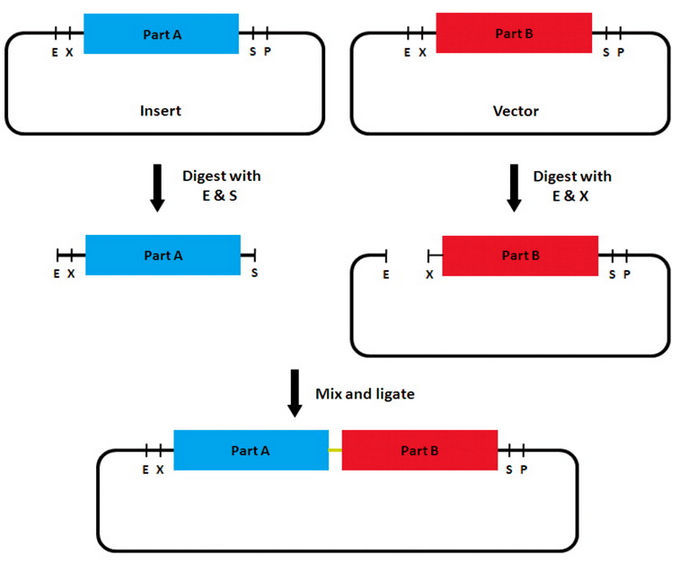
\includegraphics[width=0.8\textwidth]{images/chap4/chap4_asm_01.png}
    \caption{Standard assembly of two BioBricks (part A and part B)3. The part A plasmid is digested with EcoRI (E) and SpeI (S), the part B plasmid is digested with EcoRI (E) and XbaI (X). The sticky ends are compatible for ligation and the two parts can be assembled.}
    \label{fig:ch4asm01}
\end{figure}
\FloatBarrier
\noindent
The most significant quality of an experiment standard is its idempotency, which means that it should result in the same effect every time you apply it and that any newly added part will adhere to its assembly. \\ \\
To build complex genetic circuits, the toolkit should present a large diversity of parts to provide maximum modularity to the user, as you can see in Figure 4.2. 

\begin{figure}[!htpb]
    \centering
{{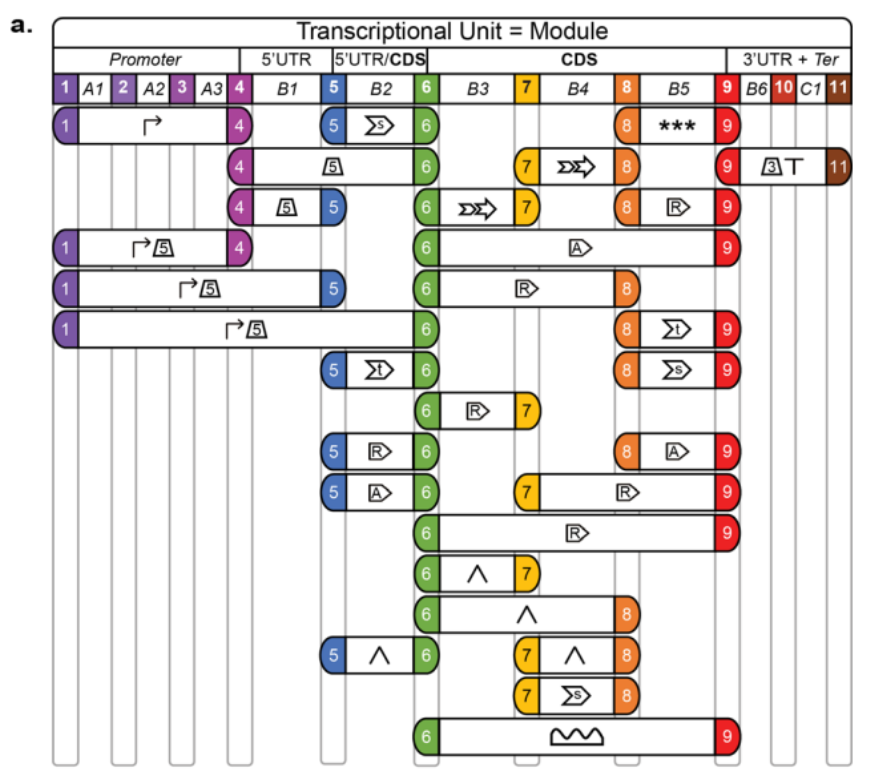
\includegraphics[width=10cm]{images/chap4/chap4_asm_02.png} }}%
    \qquad
{{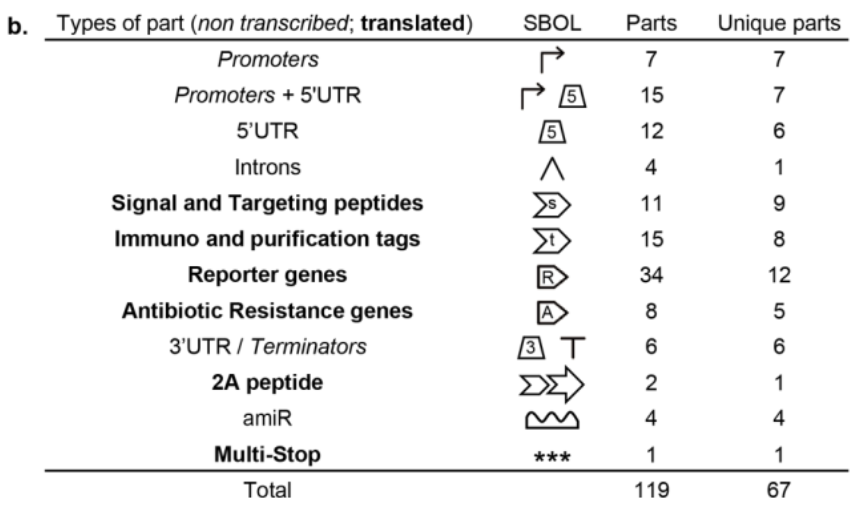
\includegraphics[width=10cm]{images/chap4/chap4_asm_03.png} }}%
    \caption{Standardised genetic parts in the \textit{Chlamydomonas} MoClo kit}%
    \label{fig:ch4asm02}%
\end{figure}
\FloatBarrier

\noindent Today, among all standardized tools, the Golden Gate Modular Cloning (MoClo) is widely used. MoClo is based on the exploitation of type II restriction enzymes to construct complex DNA sequences in only two steps. Type IIS assembly methods have been widely adopted in plant research laboratories but also for the engineering of fungi. These enzymes have the particularity to cut a few nucleotides after their recognition site. The idea is to get together multiple plasmids, each one containing one part of the gene assembly and, using only one Type II enzyme, obtain the final assembly in one step. 

\section{PhytoBricks}
\epigraph{The following section was written by Michael Burgis}{\textit{iGEM Marburg 2021}}
\subsection*{Standardization in Phototrophic Synthetic Biology}
The standardization of components in common engineering disciplines, from screw threads to printed circuit boards, is one of the key elements to facilitate both the speed of innovation and the economy of production processes. \\
The introduction of standards, in particular for the DNA assembly of characterized DNA sequences, was a landmark in microbial engineering, which heavily shaped the emerging field of synthetic biology in its early days . \\ \\
In order to facilitate the easy exchange of standardized genetic parts in plant and phototrophic chassis , the international plant science community established a common genetic syntax for DNA parts \parencite{Patron2015}. This standard is based on Type IIS restriction enzymes and enables parallel assembly of multiple DNA parts in a one-pot, one-step reaction, called Golden Gate assembly. \\ \\
Before the agreement of the  Phytobrick standard, many labs have started their own standardisation efforts by converting in house plasmids to the use of Golden Gate cloning. The GoldenBraid2.0 (GB2.0) and Golden Gate Modular Cloning (MoClo) assembly standards, which are described later in this handbook, have been adopted by the plant research communities and are partly, but unfortunately not entirely compatible.  Even small variations in the different standards prevent the exchange of parts between labs and hinder the creation of a collection of standardized, characterized, exchangeable parts for phototrophic chassis. \\ \\
The standard syntax, calles Phytobrick standard, which we would like to introduce here now, addresses exactly that, by establishing a common grammar to enable the sharing of parts throughout the plant science community, by being compatible with the most widely adopted Type IIS-based standards.

\subsection*{The Phytobrick syntax for phototrophic chassis}
The first rule of the Syntax is that all internal instances of the Type IIS restriction enzyme recognition sequence must be removed and subsequently the part has to be cloned into a compatible backbone, flanked by Type IIS restriction enzyme recognition sequences. This Backbone should also be free of the mentioned typeIIS recognition sides and additionally should also not contain bacterial resistance to ampicillin/carbenicillin or kanamycin as these are commonly utilized in the plasmids in which standard parts will be assembled into. This process is called domestication. When released from its plasmid backbone by the restriction digest with BsaI, each part contains specific, four-base-pair overhangs, known as fusion site (Figure 4.3).

\begin{figure}[!htbp]
    \centering
    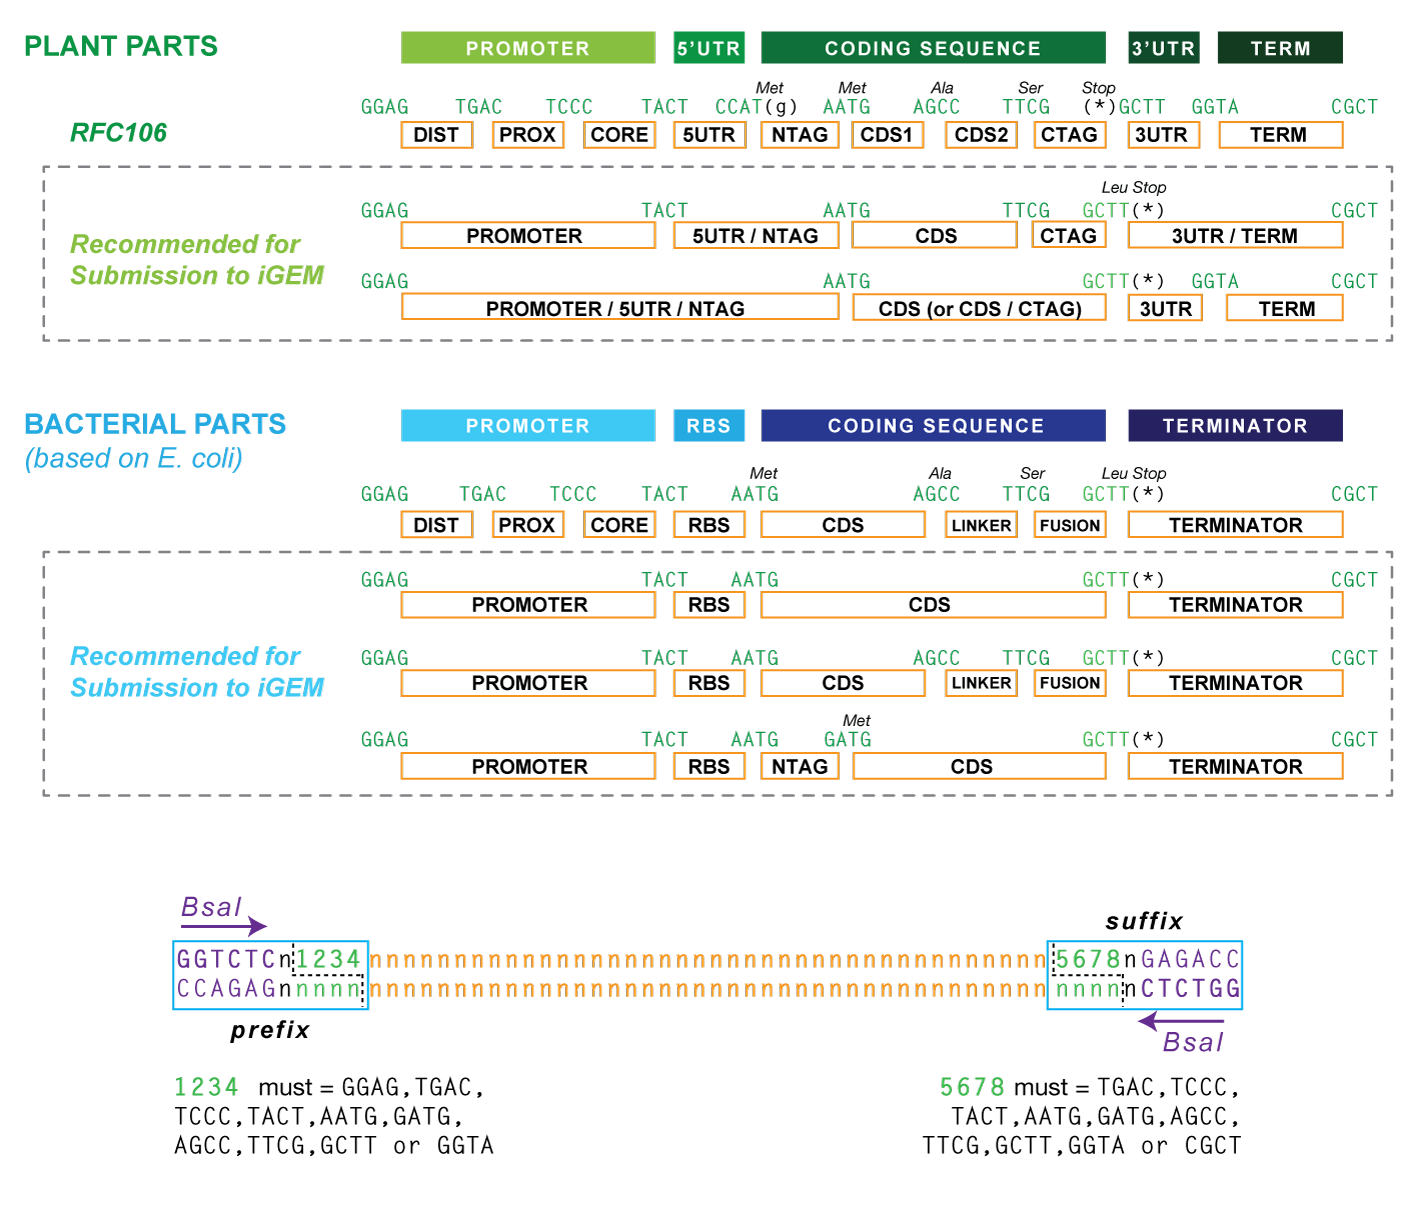
\includegraphics[width=\textwidth]{images/chap4/chap4_phy_01.png}
    \caption{Specific fusion sites of the Phytobrick syntax for the individual part types.}
    \label{fig:ch4phy01}
\end{figure}
\FloatBarrier

\noindent
A standard syntax for transcriptional units has been defined and 12 fusion points assigned. \\ \\
In both systems transcriptional units can be assembled and used directly or may be assembled with other transcriptional units to make multigene assemblies. 


\section{BioBrick RFC[10]}
\epigraph{The following section was written by Michael Burgis}{\textit{iGEM Marburg 2021}}
The Biobrick RFC[10] assembly standard was originally developed by Tom Knight was one of the most widely used assembly standards and still the majority of parts in the iGEM registry database are RFC[10] compatible, which means that they don´t contain illegal recognition/cutting sites for the restriction enzymes of this assembly standard.\\ \\
Additionally all BioBricks are flanked by standardized restriction sites, consisting of the \textbf{BioBrick} \textbf{Prefix} and \textbf{Suffix}. The Biobrick prefix contains the \textbf{E}coRI and \textbf{X}baI cutting sites, flanking the part on the left side and the Biobrick Suffix  includes \textbf{S}peI and \textbf{P}stI on the right.

\begin{figure}[!htbp]
    \centering
    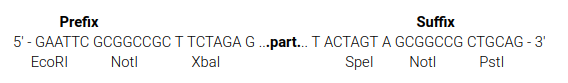
\includegraphics[width=\textwidth]{images/chap4/chap4_bio_01.png}
    \label{fig:ch4bio01}
\end{figure}
\FloatBarrier

\noindent\textbf{There is a second prefix designed for protein coding regions, because of RBS issues!}:

\begin{figure}[!htbp]
    \centering
    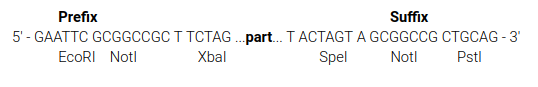
\includegraphics[width=\textwidth]{images/chap4/chap4_bio_02.png}
    \label{fig:ch4bio02}
\end{figure}
\FloatBarrier
\noindent
For the assembly of biobricks several assembly methods have been described. One of them is the 3A assembly (which stands for three antibiotic assembly), which is a method for assembling two BioBrick parts together. It differs from the common Biobrick assembly approach in that it relies on three way ligation (between the two parts and the backbone vector) for assembly rather than two way ligation between a part and a part + vector molecule.
3A assembly was designed such that gel purification of the digested parts is unnecessary,
as gel purification tends to be inefficient especially on small pieces of DNA, is slow and not easily susceptible to automation and scaling.\\ \\
It uses both positive and negative selection to reduce/eliminate the number of incorrect assemblies that give rise to colonies after transformation. One of the basic principles of this assembly method is that the sticky ends of DNA cut with two different restriction enzymes can form scars after successful ligation, which can not be recognized by either of restriction enzymes used in the assembly.\\ \\
Assembling two parts leaves the following scar: 
\begin{center}
5' [part A] TACTAGAG [part B] 3'     
\end{center}
The following description uses BioBrick RFC[10] part samples as an example.
The left part sample is in a plasmid backbone with an antibiotic resistance for antibiotic A.
The right part sample is in a plasmid backbone with an antibiotic resistance for antibiotic B.
A linearized plasmid backbone is selected with neither resistance A nor B. It has AB resistance C. 


\begin{figure}[!htbp]
    \centering
    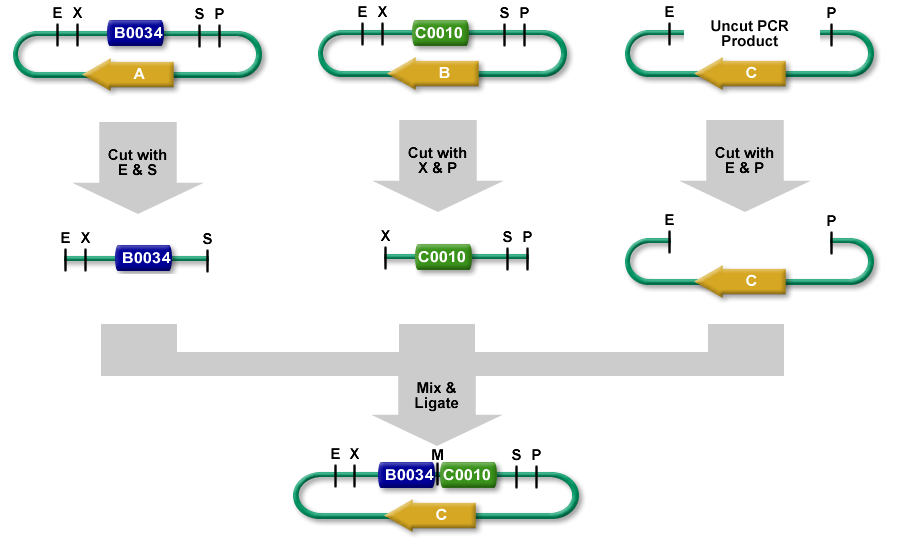
\includegraphics[width=\textwidth]{images/chap4/chap4_bio_03.png}
    \label{fig:ch4bio03}
\end{figure}
\FloatBarrier


\subsection*{Restriction Digests}
The left part sample is cut out with \textbf{E}coRI and \textbf{S}peI. \\ 
The right part sample is cut out with \textbf{X}baI and \textbf{P}stI. \\
The linearized plasmid backbone is cut with \textbf{E}coRI and \textbf{P}stI. \\
All 3 restriction digests are heated to heat kill all of the restriction enzymes. \\ \\
An equimolar quantity of all 3 restriction digest products are combined in a ligation reaction.
The desired result is the left part sample's SpeI overhang ligated with the right part sample's XbaI overhang resulting in a scar that cannot be cut with any of our enzymes. \\
The new composite part sample is ligated into the construction plasmid backbone at the EcoRI and PstI sites. \\
When the ligation is transformed into cells and grown on plates with antibiotic C, only colonies with the correct construction survive. \\ \\
As described above, each cycle of BioBrick/3A assembly joins just two parts together and several rounds of cloning are necessary to construct a full functional transcriptional unit, which is far slower than more recent assembly techniques such as typeIIS based methods or Gibson assembly. Another major concern with BioBrick RFC[10] is that it does not facilitate the assembly of proteins,as the traditional 8bp scar creates a frame-shift, while the alternate 6bp scar includes a stop codon. If you wish to assemble proteins you will want to use an RFC designed specifically for protein assembly.


\section{iGEM Type IIS RFC[1000]}
\epigraph{The following section was written by Yasoo Morimoto}{\textit{iGEM Marburg 2021}}
\subsection*{Introduction}
The iGEM Type IIs assembly provides flexibility and the possibility of a high throughput workflow, it takes advantage of Type IIs restriction enzymes to directionally assemble several genetic parts in a one-pot, one-step reactions. This standard was based on previous works that also put forth similar cloning methods (Moclo, Loop, golden braid). \\ \\ 
Enzymes used: BsaI, SapI \\
Antibiotics used: Chloramphenicol, Kanamycin

\subsection{Type IIS}
Type IIs Restriction enzymes have the special ability to cut outside of their recognition site in a directional fashion, this enables for the selection of arbitrary overhangs and for scarless ligation. \\ \\

\begin{figure}[!htbp]
    \centering
    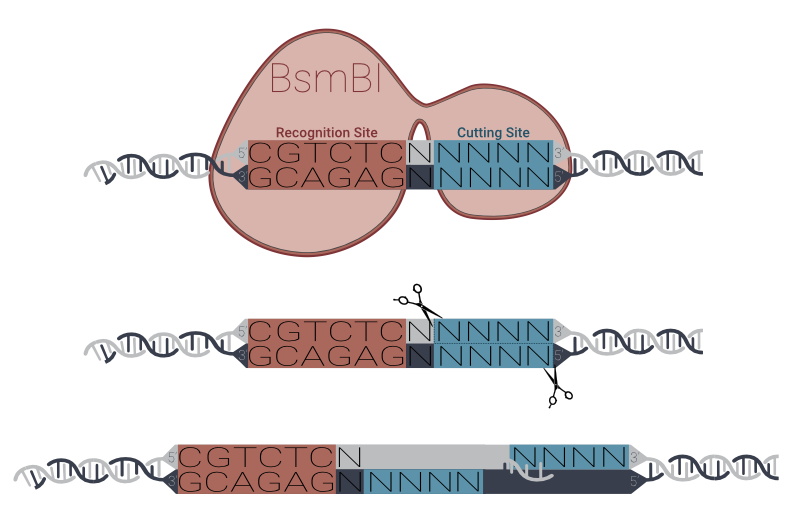
\includegraphics[width=\textwidth]{images/chap4/chap4_rfc1000.png}
    \label{fig:ch4rfc1000}
\end{figure}
\FloatBarrier

 \noindent
The overhangs (fusion sites) used for each part have been standardized for greater interchangeability; Newer Assembly systems have mostly adopted the fusion sites proposed by the MoClo paper \parencite{Weber2011}, therefore, parts in the registry can be used by different systems, given that they don’t contain Illegal cutting sites. RCF 1000 also uses the MoClo fusion sites for its parts. \\ \\
The standard uses the enzymes BsaI and SapI, so compatible parts can’t have these restriction sites insite their sequence. Note that standard compatibility doesn’t depend on the prefix/suffix surrounding the part, those can be arbitrarily chosen depending on the desired assembly system, but if a part has for example a bsaI recognition site (5'...GGTCTC N NNNN...3’) in its sequence, it won’t work in the Type IIS assembly, independently of the prefix/suffix. \\ \\
The assembly process works by successively cloning genetic parts from level 0 plasmids in higher order constructs. Level 1 plasmids take in transcription units (TUs), which can be in turn assembled into Multi-Transcription units (MTUs) in level 2 plasmids.

\subsection*{Level 0}

Parts stored in the level 0 plasmid pSB1C00 can be cut out with BsaI, the fusion sites left on the part are correspondent to the part’s position in the transcription unit:
table of the fusion sites
\begin{figure}[!htbp]
    \centering
    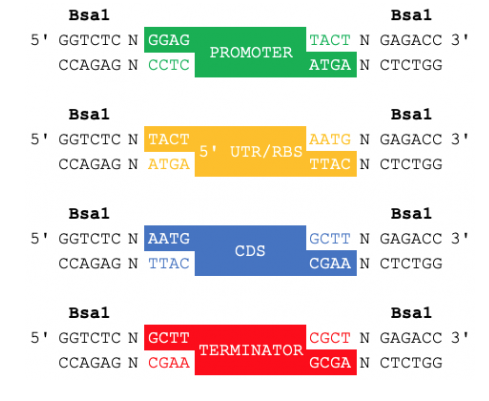
\includegraphics[width=0.8\textwidth]{images/chap4/chap4_typ_01.png}
    \label{fig:ch4typ01}
\end{figure}
\FloatBarrier
\noindent
This allows for the assembly of all parts of a TU in the correct order in a one-pot reaction. 
The backbone used for storing parts (pSB1C00) has a chloramphenicol resistance cassette. After the assembly with the selected parts and one level 1 acceptor vector (pOdd), the TU will be flanked by SapI restriction sites.
\begin{figure}[!htbp]
    \centering
    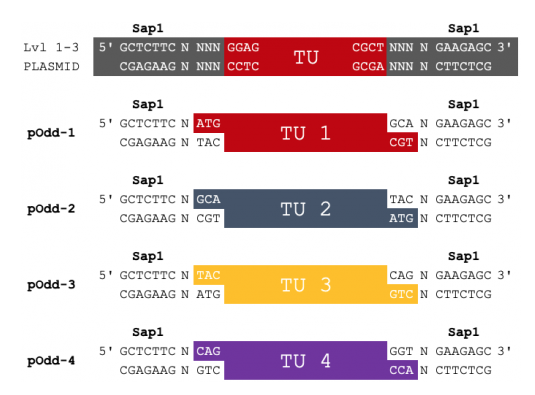
\includegraphics[width=0.8\textwidth]{images/chap4/chap4_typ_02.png}
    \label{fig:ch4typ02}
\end{figure}
\FloatBarrier
\noindent
The fusion sites on each plasmid determine the position of each TU in the final level 2 construct.\\ \\
To domesticate a part - i.e. clone it into the Universal Acceptor Vector (pSB1C00) - it must be flanked with the right vector fusion sites. The easiest way to achieve this is using extension PCR to introduce these features as prefix/suffix to the part. The next step is using SapI to clone it into pSB1C00.

\subsection*{Level 1}
The RFC 1000 Standard offers 4 level 1 plasmids, their SapI restriction sites leave 3bp fusion sites, which allow for the assembly of multi-gene units of up to 4 TUs in a level 2 assembly. This number can be expanded by creating new level 1 backbones or by performing further cloning steps after level 2. The fact that the backbones used already conform to Loop make it easy to assemble larger constructs. \\ \\
The Backbones used for level 1 plasmids are pSB1K01-pSB1K04, they are based on the pOdd backbones from the loop assembly. 

\subsection*{Level 2}
The next step is assembling TUs into a level 2 backbone to build multi-gene units (MTUs), the Type IIs standard offers four plasmids for this job, which are also based on the Loop plasmids pEven1 - pEven4. The TUs can then be assembled in level 2 plasmids using SapI. 

\epigraph{The following section was written by Yasoo Morimoto}{\textit{iGEM Marburg 2021}}
\subsection{Modular Cloning}
\noindent
Firstly introduced by \parencite{Weber2011}, the MoClo Assembly is based on the Golden Gate system \parencite{Engler2008} for building multi-gene constructs in a one step, one pot reaction. It relies on the ability of type IIs enzymes to cut outside of their recognition site to create unique and standardized overhangs. These overhangs, in turn, dictate the position of each part in the plasmid. This standard includes unique overhangs for promoters, 5’UTRs, signal peptides and more; the only two enzymes used are BsaI, Esp3I and BpiI. Plasmids code for spectinomycin, ampicillin or kanamycin \parencite{Weber2011}.

\subsubsection{Construct Design}
Transcription units (TUs) start with the promoter upstream overhang (GGAG) and end with the Terminator downstream overhang (CGCT). While restriction enzymes in level 0 plasmids have identical fusion sites, level 1 plasmids leave unique sequences after cleavage for directional cloning. The MoClo toolbox provides level 1 destination vectors with 7 different overhangs, so that one can assemble multi-gene constructs  with up to 6 TUs (positions 1 to 7) in a single reaction. This is especially attractive for creating more complicated metabolic pathways. 

\begin{figure}[!htbp]
    \centering
    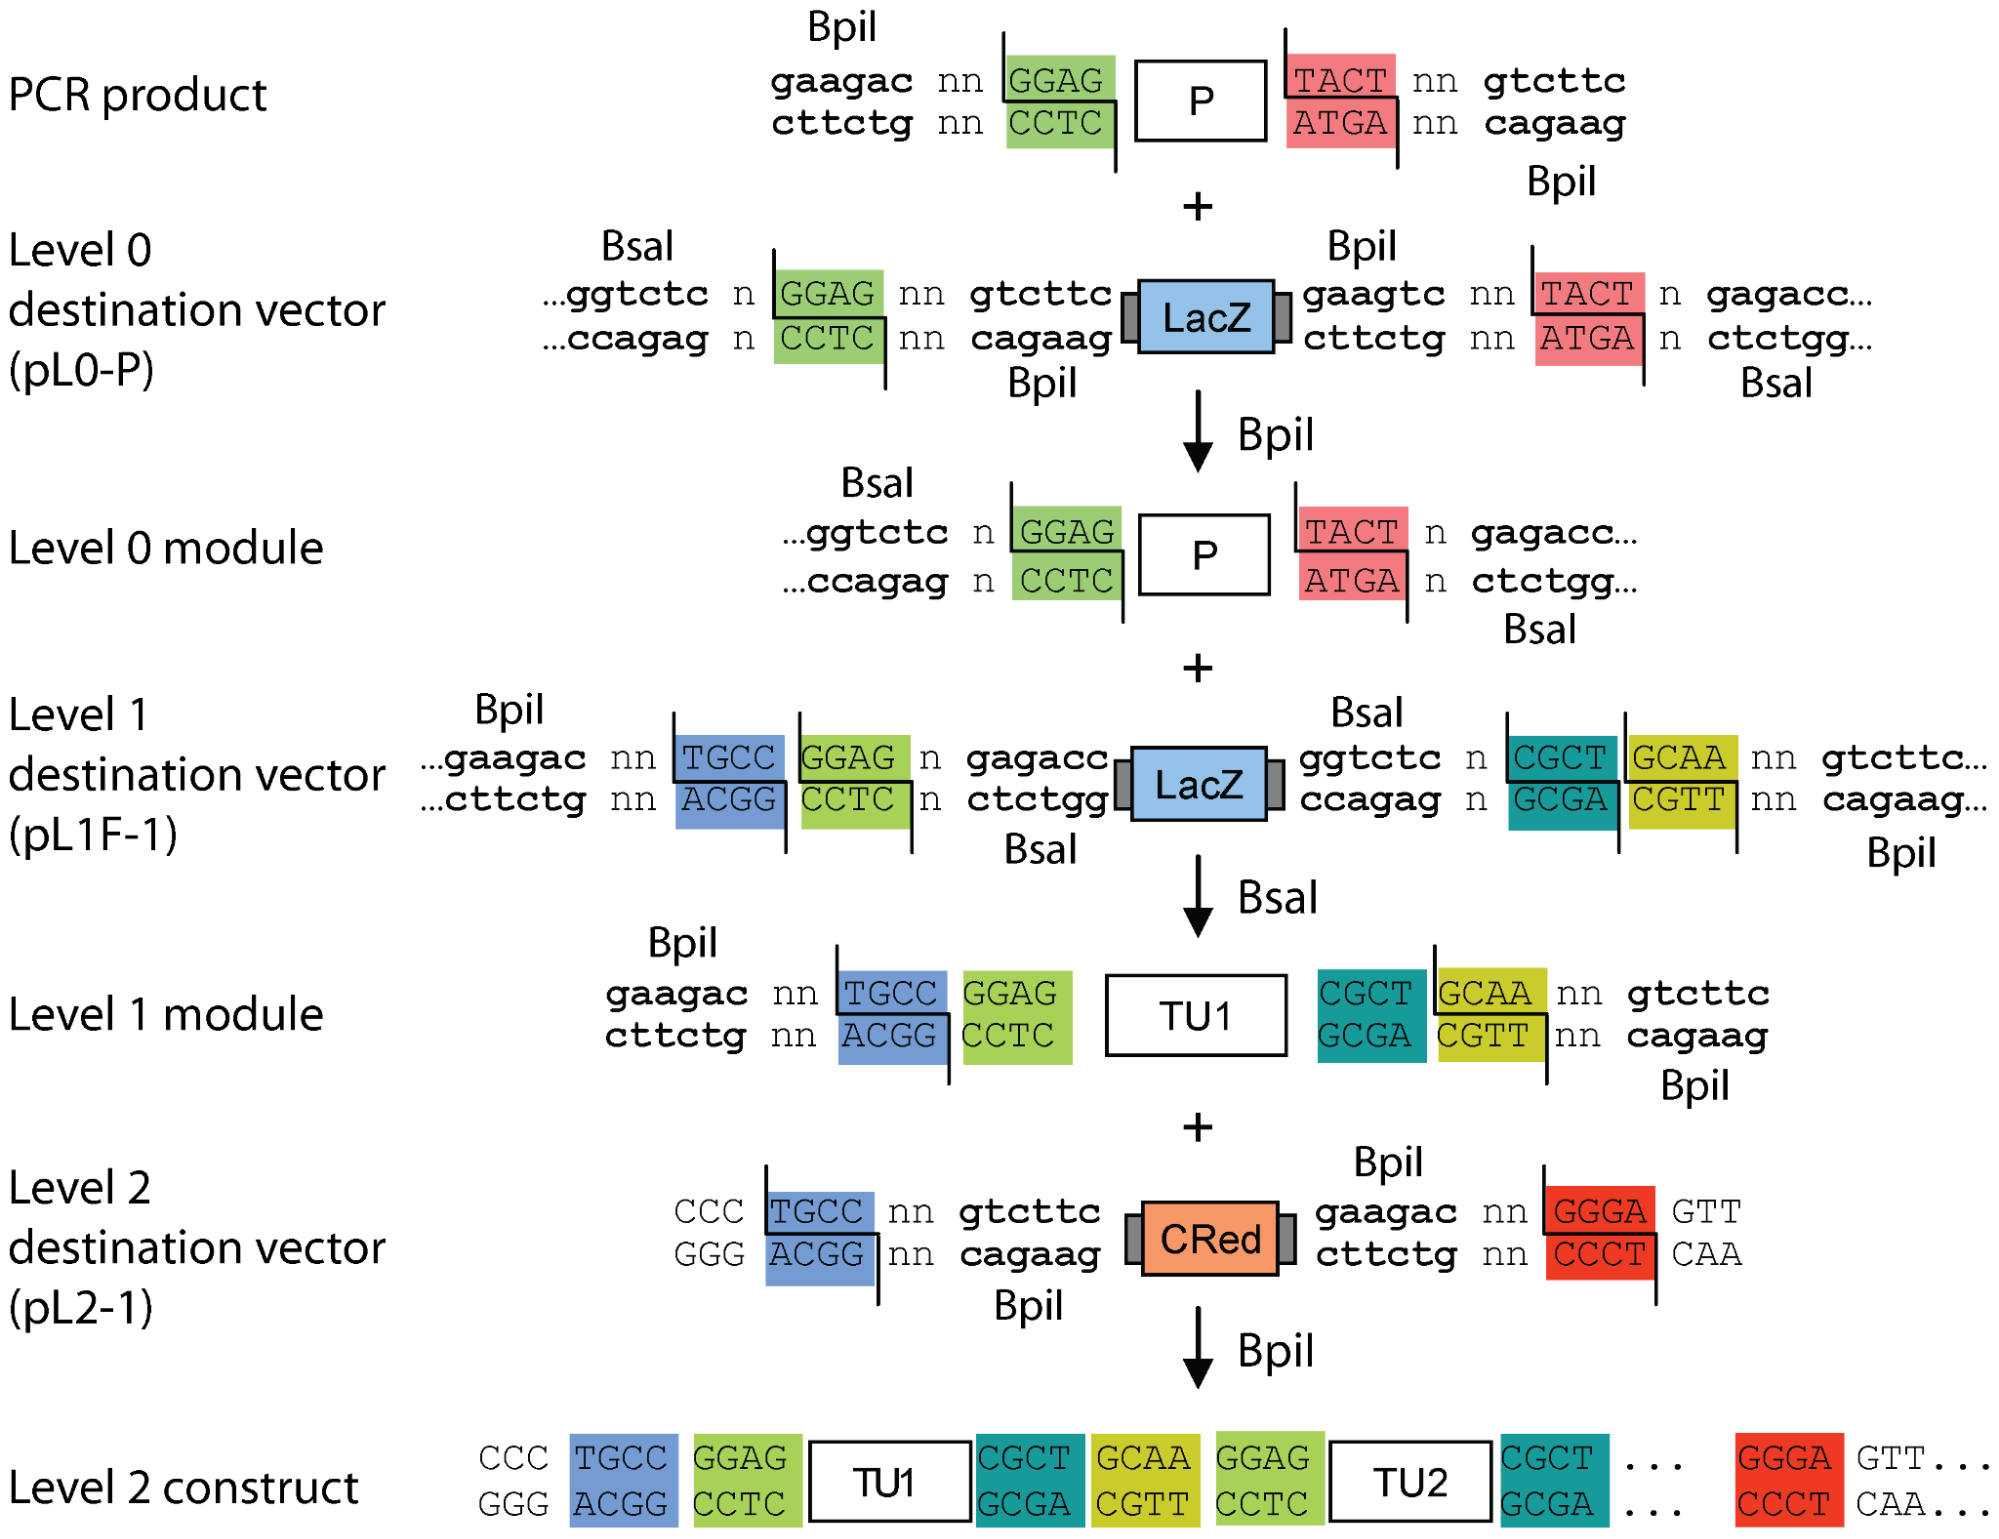
\includegraphics[width=\textwidth]{images/chap4/chap4_moclo_01.png}
    \label{fig:ch4mcl01}
\end{figure}
\FloatBarrier

\noindent The number of TUs in a level 2 plasmid is not limited to 7, though; because the fusion sites are organized in a “circular” logic, the downstream overhang at position 7 is compatible with the upstream position 1 insert. So it is theoretically possible to indefinitely extend the plasmid with new TUs by adding new reaction steps. A second set of level 1 destination plasmids allows for insertion of TUs in the reverse orientation at any position. \\ \\
To bridge the gap between the last used level 1 module (which has an variable upstream fusion site depending on its position number) and the backbone, an End Liker is required. These parts have the same selection markers as 

\epigraph{The following section was written by Yasoo Morimoto}{\textit{iGEM Marburg 2021}}
\subsection{Loop Assembly}
One of the great benefits of working with Type IIs cloning is the potential for highly standardized part design, allowing for the easy exchange between working groups. On top of this benefit, Loop Assembly \parencite{Pollak2020} also allows for an uncomplicated assembly of large constructs containing several transcription units (TUs), through recursive cloning the size of the final sequence can grow indefinitely.  Furthermore, the system is also compatible with long-overlap assembly, TUs can also be cloned using Gibson Assembly.

\subsubsection{Components}
Loop Assembly works by alternating a set of four odd number plasmids (pOdd) with a set of four even numbered plasmids (pEven). Both types of plasmids possess SapI and BsaI cutting sites, albeit in different orientations. \\ 

\textbf{pEven1 - 4}
\begin{itemize}[noitemsep,topsep=0pt]
    \item Spectinomycin
    \item SapI for cloning step
    \item LacZ Dropout
    \item UNSp1 - 5
    \item UNSx
\end{itemize} 


\textbf{pOdd1 - 4}
\begin{itemize}[noitemsep,topsep=0pt]
    \item Kanamycin
    \item BsaI for cloning step
    \item LacZ Dropout
    \item UNSp1 - 5
    \item UNSpx
\end{itemize}  


\textbf{POdd Spacer}
\begin{itemize}[noitemsep,topsep=0pt]
    \item 200bp random DNA spacer
    \item Kanamycin
    \item BsaI for cloning step
\end{itemize} 


\textbf{PEven Spacer}
\begin{itemize}[noitemsep,topsep=0pt]
    \item 200bp random DNA spacer
    \item Kanamycin
    \item SapI for cloning step
\end{itemize} 
\mbox{} \\
All plasmids contain the pMB1 origin of replication.

\subsubsection{Cloning Method}
As a MoClo Standard, Loop relies on Level 0 parts with compatible overhangs to build it’s transcription units. pOdd plasmids are receiver to level 0 parts compatible to the PhytoBricks standard \parencite{Patron2015}. Cutting them with BsaI leaves the promoter CCTC and terminator CGCT overhangs on the backbone, this allows the cloning of one TU (level 1 construct). To clone into a level 2 plasmid, four TUs cloned in pOdd1 - pOdd4 are assembled in a reaction with SapI to clone in a level 2 pEven plasmid. Each POdd plasmid defines the position of it’s TU through the fusion sites left by the SapI restriction reaction, the sites are named $\alpha, \beta, \gamma, \epsilon, \omega$, and all pEven backbones have $\alpha$ and $\omega$ fusion sites for the first and the last TUs. 

\begin{figure}[!htbp]
    \centering
    \caption{Adapted from \parencite{Pollak2020}.}
    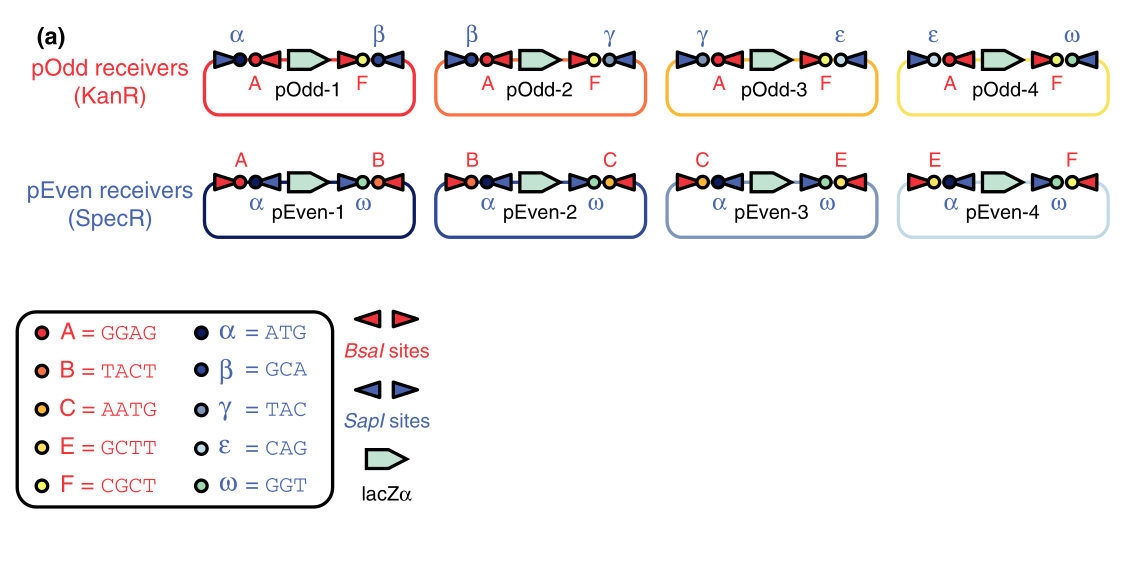
\includegraphics[width=\textwidth]{images/chap4/chap4_loop_01.png}
    \label{fig:ch4loop01}
\end{figure}
\FloatBarrier

\noindent
The important feature of Loop comes now: you can just keep going with another round of cloning. With four level 2 pEven plasmids it is possible to set up a level 3 reaction and  assemble 16 TUs in a pOdd plasmid. Here, the fusion sites left by BsaI determine the position of each insert. Because of the way the overhangs are layed out, each cloning step must introduce four inserts, this exponentially increases the amount of TUs cloned. For use-cases that need a smaller number of TUs, the system offers a “Universal Spacer” that can be cloned in any receiver plasmid, this Universal Spacer contains 200bp random DNA devoid of BsaI or SapI cutting sites. 

\begin{figure}[!htbp]
    \centering
    \caption{Adapted from (Pollak et al., 2019)}
    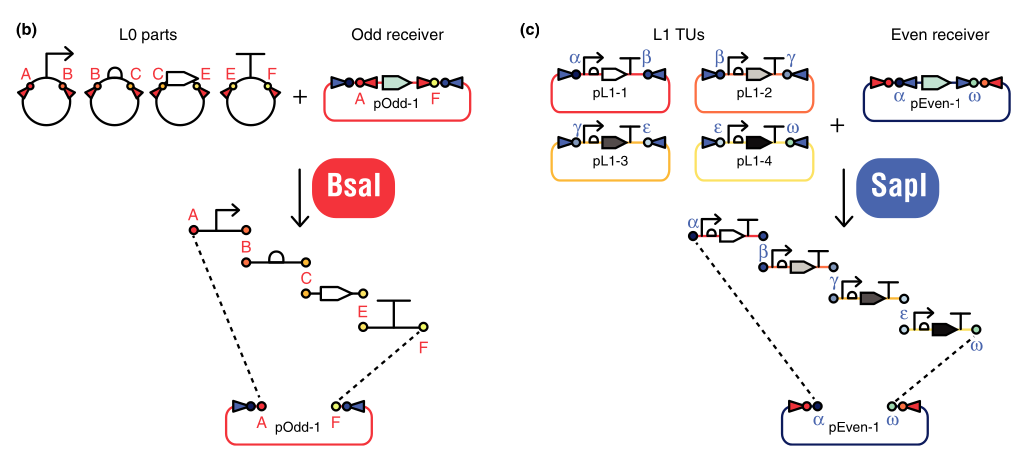
\includegraphics[width=\textwidth]{images/chap4/chap4_loop_02.png}
    \label{fig:ch4loop02}
\end{figure}
\FloatBarrier

\subsubsection{Long Overlap Assembly} 
In addition to Type IIs, long overlap assembly cloning methods have also gained popularity in the synthetic biology community. Methods like Gibson Assembly \parencite{Gibson2008} offer a low cost and fast cloning method capable of assembling several fragments in a one-pot isothermal reaction. Furthermore, new methods aim to streamline this process by introducing standardized unique nucleotide sequences (UNSs) that allow us to combine several TUs in a larger construct \parencite{Pollak2020} \parencite{Torella2013}. \\ \\
Flanking the cutting sites for BsaI and SapI, the Loop Plasmids include UNSs for the assembly of multi-gene constructs using Gibson Assembly.

\begin{figure}[!htbp]
    \centering
    \caption{Adapted from \parencite{Pollak2020}.}
    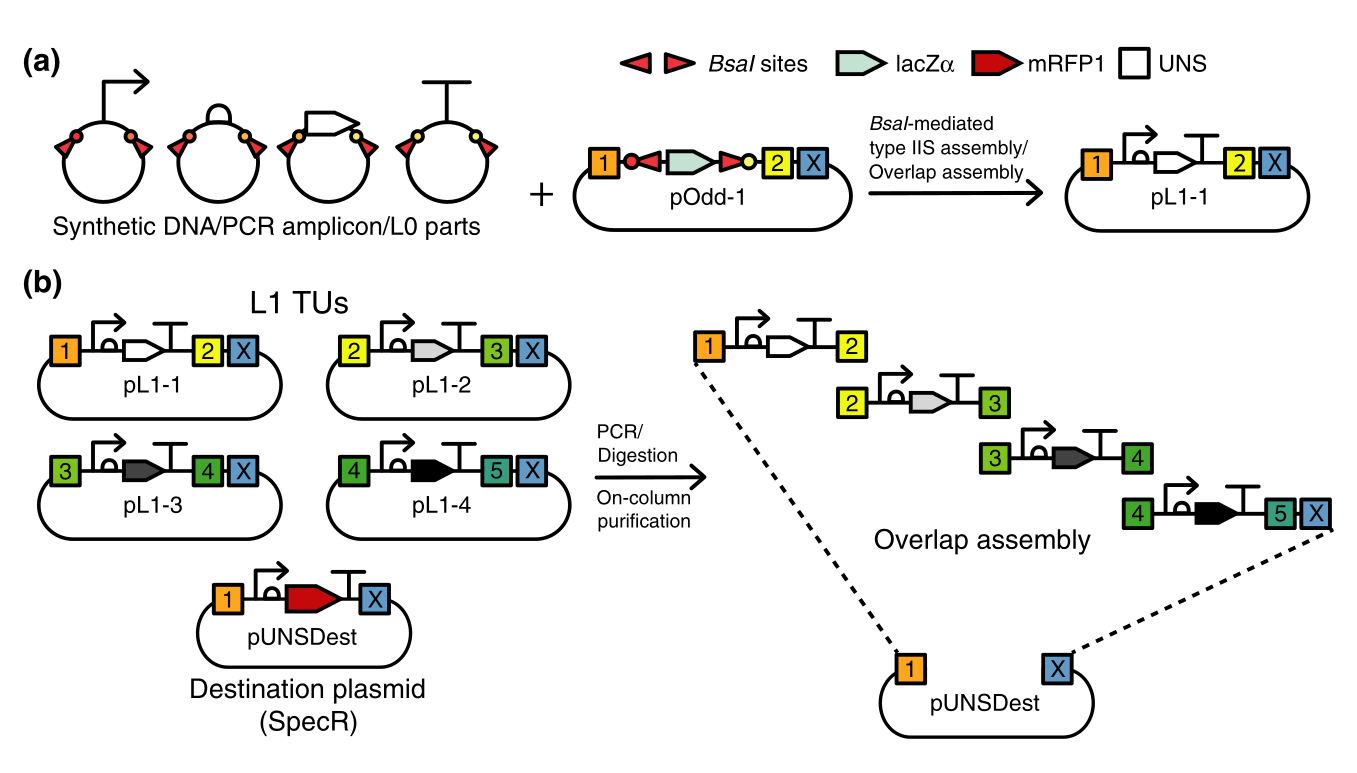
\includegraphics[width=\textwidth]{images/chap4/chap4_loop_03.png}
    \label{fig:ch4loop03}
\end{figure}
\FloatBarrier


\epigraph{The following section was written by Paul Goffing}{\textit{iGEM Bielefeld-CeBiTec 2021}}
\subsection{Mobius Assembly}
\subsubsection{Introduction}
The Mobius Assembly is a recent adaption of the Golden Gate cloning system and Modular Cloning, developed by Andreas Andreou at Naomi Nakayama’s lab \parencite{Andreou2018}. In their publication, the authors state that the Mobius Assembly makes Golden Gate more versatile without compromising capacity. In addition, especially interesting for iGEM Teams working with plants, the used backbones are binary plasmids. This means that Mobius Assembly can be used for Agrobacterium-mediated transformation of plants. The developers of Mobius Assembly expanded in their method standards which were set by iGEM: the backbones are based on the iGEM standard vectors pSB1C3 and pSB1K3 and the choice of overhangs is based on Phytobricks. Thus, Mobius Assembly is compatible with all iGEM Type IIS standard parts.\\ \\
Enzymes used: BsaI, AarI, EcoRI, PstI, T4 DNA Ligase \\
Antibiotics used: Chloramphenicol, Kanamycin, Spectinomycin
\subsubsection{Basic Principle}
The Mobius Assembly basically works like iGEM Type IIS cloning. Basic parts are assembled in Level 0 vectors (mUAV - Mobius Universal Acceptor Vector). They can be assembled to transcriptional units (TUs) in Level 1. TUs from Level 1 can be combined in Level 2. If more TUs need to be combined or added later, it is possible to switch back and forth between Level 2 and Level 1. This switching back and forth is where the name Mobius Assembly comes from. \\ \\
Let me remind you how Type IIS cloning works. Type IIS restriction enzymes recognize a specific sequence and cut at a different position, creating sticky ends. This gives the opportunity to create a large number of different overhangs by using only one restriction enzyme. At the position, where two basic parts need to be combined, they share the same overhang. At the same time, the same overhang is only used at one ligation site between basic parts. This order of different overhangs results in two things: First, all basic parts will always be assembled in the correct order. Second, basic parts are exchangeable, if they have the same overhangs. To facilitate the latter aspect, Phytobricks standardised the use of overhangs, shown in figure 1B. \\ \\
In comparison to other cloning methods, like Gibson Assembly or Biobrick standard, it is quite easy and fast to assemble large vectors containing many different basic parts using Mobius Assembly.
\subsubsection{Cloning}
If you decide to use mobius assembly, I strongly recommend to follow the instructions from this Springer protocol \parencite{Andreou2020}. \textbf{Important note}: The figure in this Springer protocol has an error! The first overhang must be GGAG and not GAAG!
\paragraph{Level 0 cloning} \mbox{}\\
The first step in Mobius Assembly is the creation of Level 0 vectors containing all the basic parts you want to use. The Level 0 empty vector is called mUAV (Mobius Universal Acceptor Vector). It has a chloramphenicol resistance and carries the amilCP gene as a negative selection marker, which gives the colonies carrying the empty vector a strong purple colour. This makes it possible to screen colonies without the use of expensive chemicals like IPTG and X-Gal for screening and also allows the use of strains which don’t have a lacZ deletion. mUAV is not a binary vector. So this vector cannot be used to transform plants via Agrobacteria.\\ \\
The cloning of your parts into mUAV is quite simple (see Figure 4.7 A: for a graphical representation).
\begin{enumerate}
\item Amplify your part using primers with overhangs, which introduce the overhangs for Level 1 cloning and the recognition sites for AarI and BsaI. Purify the PCR product.
\item Digest mUAV and your PCR product with AarI, ligate with T4 DNA Ligase (in a one pot reaction).
\item Transform the ligated plasmids into E. coli (Top10 or DH5α).
\item Control restriction digest with EcoRI and PstI.
\item Sequence positive clones (this is the only necessary sequencing step in Mobius Assembly)
\end{enumerate}

\begin{figure}[!htbp]
    \centering
    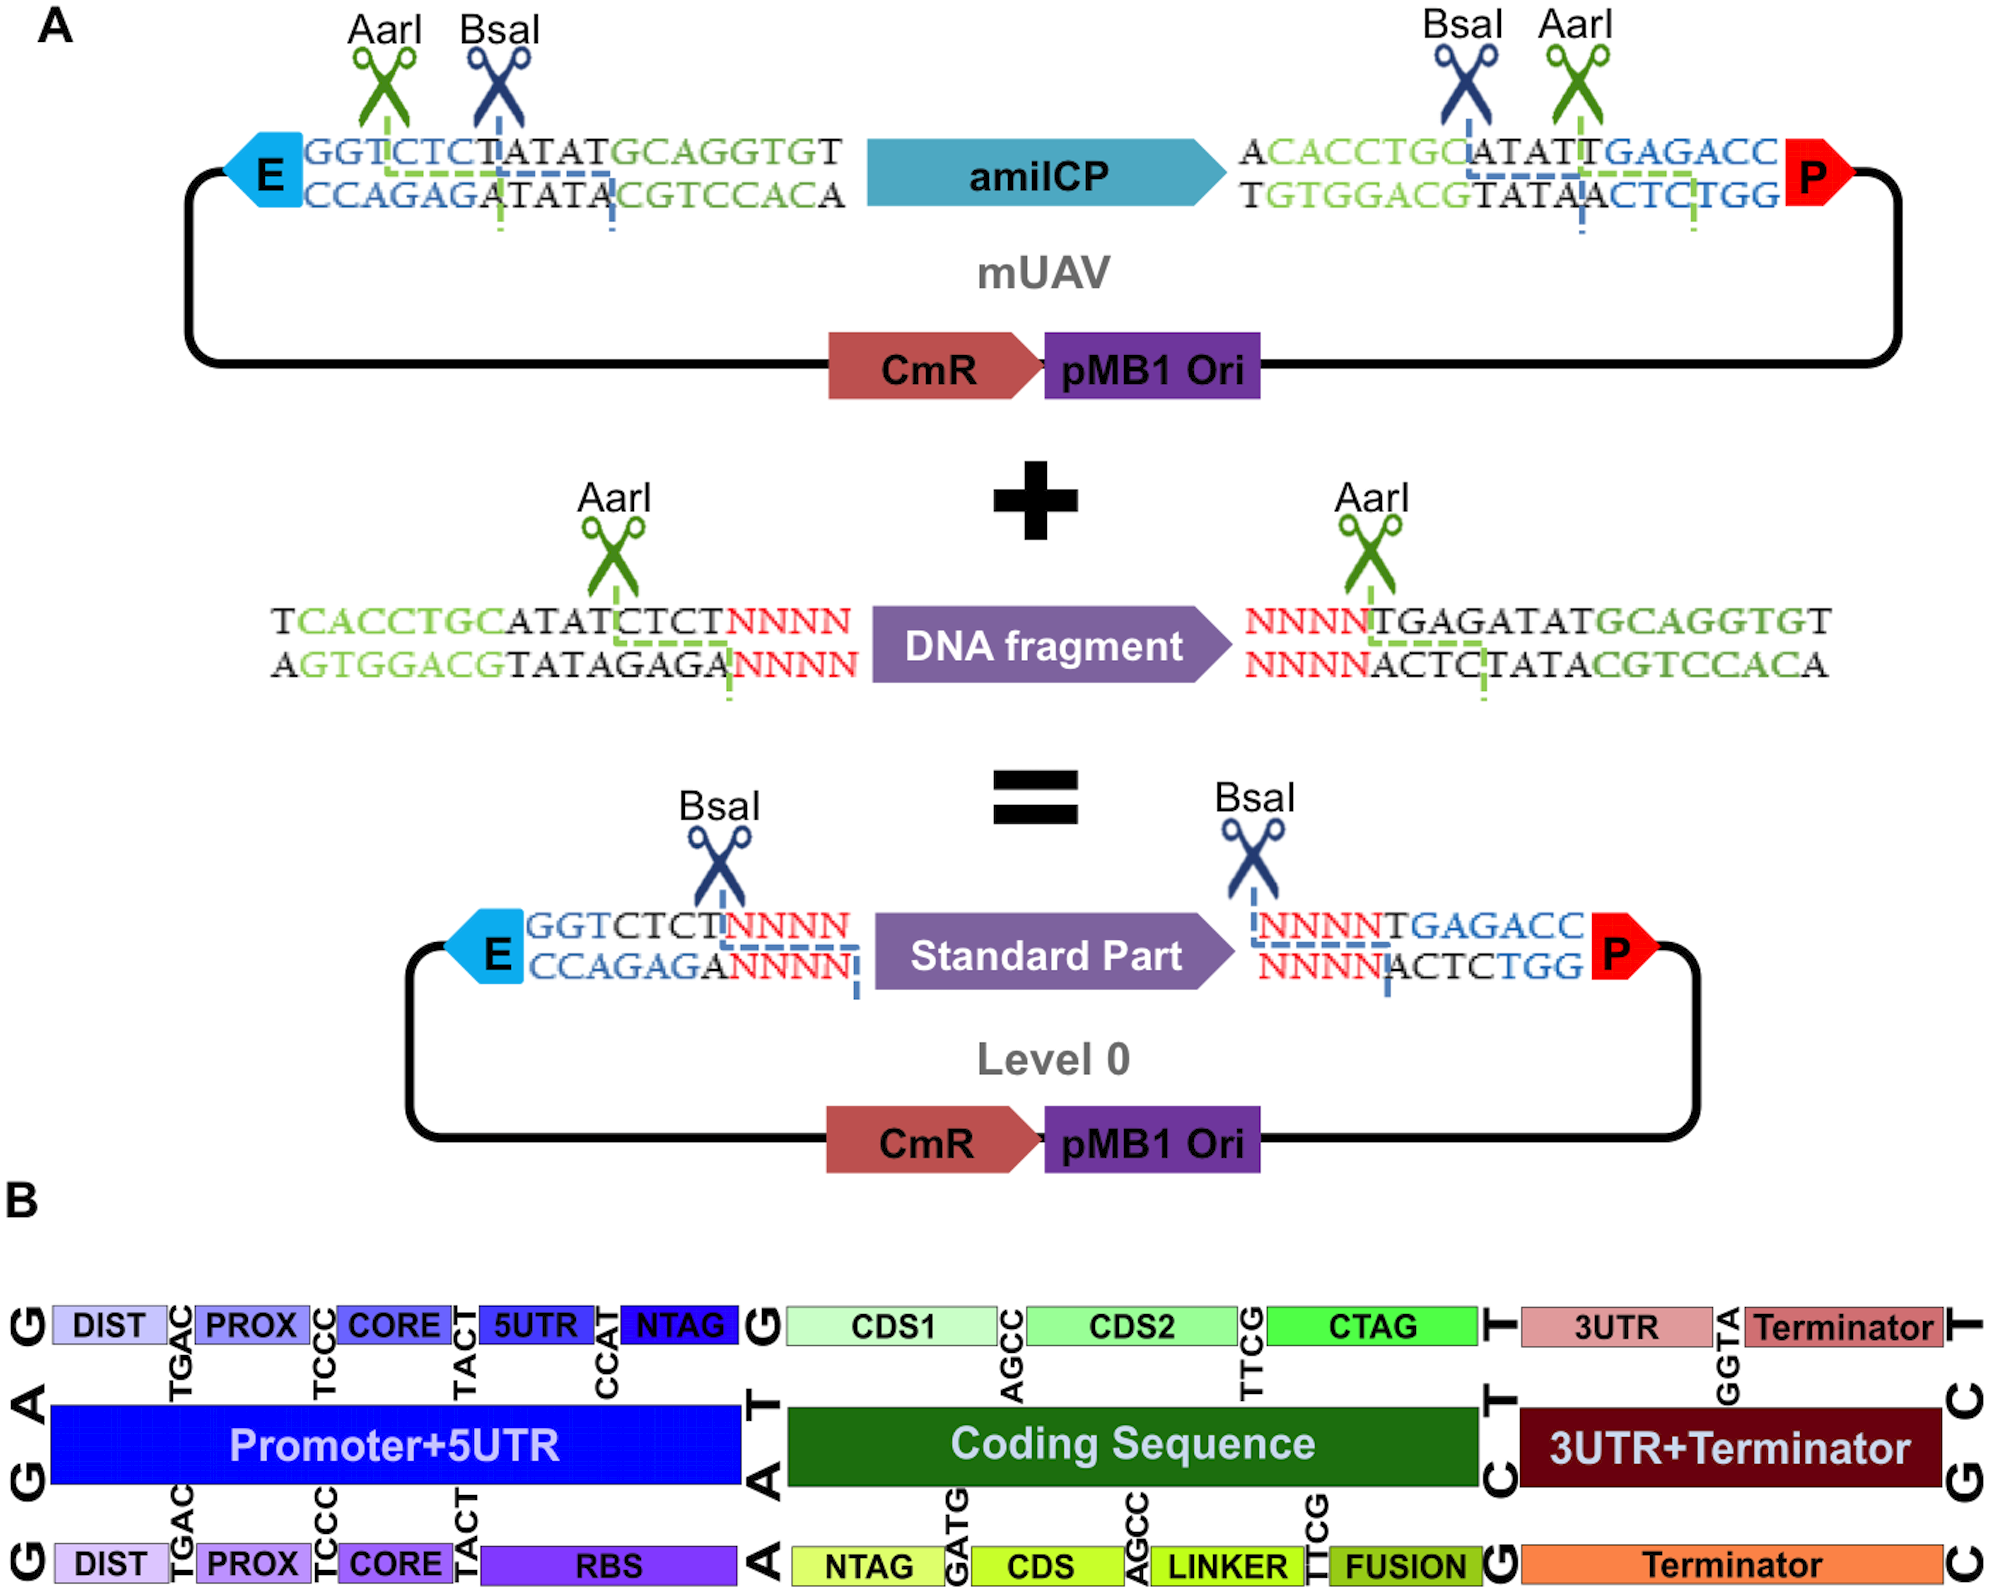
\includegraphics[width=\textwidth]{images/chap4/chap4_mob_01.png}
    \label{fig:ch4mob01}
    \caption{Adapted from \parencite{Andreou2018}.}
\end{figure}
\FloatBarrier

\paragraph{Level 1 cloning} \mbox{} \\
In Level 1, basic parts from Level 0 can be combined to form a transcriptional unit (TU). As described above, the overhangs 5’ and 3’ of the parts determine the order in which they are combined. The 5’ overhang of the promotor needs to be GGAT and the 3’ overhang of the terminator needs to be CGCT. This makes it possible to ligate the parts in Level 1. \\ \\
There are four Level 1 acceptor vectors, A, B, Γ, Δ (the greek capital letters Alpha, Beta, Gamma and Delta). One always starts with the first Level 1 acceptor vector, Level 1A. If it is necessary to assemble multiple TUs in Level 2, they will be assembled using the vectors B, Γ and Δ. \\ \\
The Level 1 vectors are based on pSB1K3. With the assembly of a TU, the spisPink gene is replaced. Thus, colonies with the empty vector are pink while colonies with vectors with insert are white. As in Level 0 cloning the spisPink works as negative selection marker. The vector carries a resistance against kanamycin.\\ \\
The cloning of Level 1 is as simple as the cloning of Level 0:
\begin{enumerate}
    \item Digestion of the Level 1 accepter vector together with all the basic parts one wants to assemble to a TU with BsaI, ligation with T4 DNA Ligase (in a one pot reaction).
    \item Transform the ligated plasmids into E. coli (Top10 or DH5α).
    \item Control restriction digest with EcoRI and PstI.
\item Sequencing of positive clones is only necessary, if Level 2 cloning fails.
\end{enumerate}
\paragraph{Level 2 cloning} \mbox{}\\
In Level 2 up to 4 TUs can be assembled to form a multi-TU-construct. If there is the need to assemble more than 4 TUs, multiple Level 2 vectors (containing multiple TUs) can be combined in Level1 afterwards. Level 2 cloning is very similar to Level 1 cloning. There are the different acceptor vectors A, B, Γ and Δ. Also, one starts assembling in the first vector, A. Level 2 requires additional auxiliary plasmids as middle-to-end-linkers or end-to-end-linkers. These auxiliary plasmids need to be added together with the Level 1 vectors to the ligation reaction. For the assembly of 4 TUs in Level 1A, the plasmid Auxiliary A needs to be added, for the assembly of 4 TUs in Level 1B, the plasmid Auxiliary B needs to be added, and so on. Additionally, there are three different middle-to-end linker auxiliary plasmids, Auxiliary 1, Auxiliary 2 and Auxiliary 3, for the assembly of 1, 2 or 3 TUs in Level 2. \\ \\
All Level 2 vectors carry a spectinomycin resistance and are again based on pSB1C3. The negative selection marker sfGFP colours the negative transformands yellow. \\ \\
\begin{enumerate}
    \item Digestion of the Level 1 accepter vector together with all the basic parts one wants to assemble to a TU and the proper auxiliary plasmid with AarI, ligation with T4 DNA Ligase (in a one pot reaction).
    \item Transform the ligated plasmids into E. coli (Top10 or DH5α).
    \item Control restriction digest with EcoRI and PstI.
\end{enumerate}
\paragraph{Primer Design} \mbox{} \\
For Level 0 cloning, the basic parts need to be inserted using specific overhangs. Also, additional recognition sequences for the Type-IIS enzymes need to be added. Therefore it is necessary to either order gene synthesis directly with the suitable overhangs or to amplify the fragment using primers with these overhangs and a proof-reading polymerase. A step-by-step introduction into primer design is also included in the Springer protocol mentioned above. This Springer protocol also explains all the other experimental procedures step-by-step. \\ \\
If the sequence you want to amplify contains recognition sites for AarI or BsaI, it is necessary to domesticate the sequence, which means to remove the recognition sites. For this, the sequence 5’ of the recognition sequence and 3’ of the recognition sequence are amplified with primers, which replace one nucleotide, so that the amino acid is still the same, but the recognition site is destroyed. There again the additional overhangs for the recognition sites of the Type-IIS enzymes are added. In the end, both PCR products are used together for Level 0 cloning.

\epigraph{The following section was written by Michael Burgis}{\textit{iGEM Marburg 2021}}
\subsection{Golden Braid}
In the beginning of the development of TypeIIS assembly strategies, the Modular Cloning standard and the Golden Braid system were designed completely independently and were published one after each other. Therefore each system has not considered the standards of the other system, which made them incompatible. 
The main features of the original Golden Braid system are that it is based on the type IIS restriction enzymes, allows the indefinite growth of reusable gene modules, consists of a set of just four destination plasmids (pDGBs) designed to incorporate multipartite assemblies made of standard DNA parts \parencite{Sarrion-Perdigones2011}.  \\ \\
In contrast to the Modular Cloning system, modules are combined \textbf{binarily} to build increasingly complex multigene constructs, \textbf{instead of the hierarchical/multipartite assembly cloning approach}. \\ \\
Nowadays the newer versions of the Golden Braid system \parencite{Sarrion-Perdigones2013} are far more used than the original, as it combines some advantages of the Modular cloning system, such as the standardized basic parts and the fast assembly of single transcription units combined with the simplicity of the original binary Golden Braid system, which just needs a few vectors, instead of a large number of acceptor vectors and end-linkers. Additionally this updated version introduced the concept of the universal acceptor vector for parts, which is also continuously used in the Phytobrick standard.

\begin{figure}[!htbp]
    \centering
    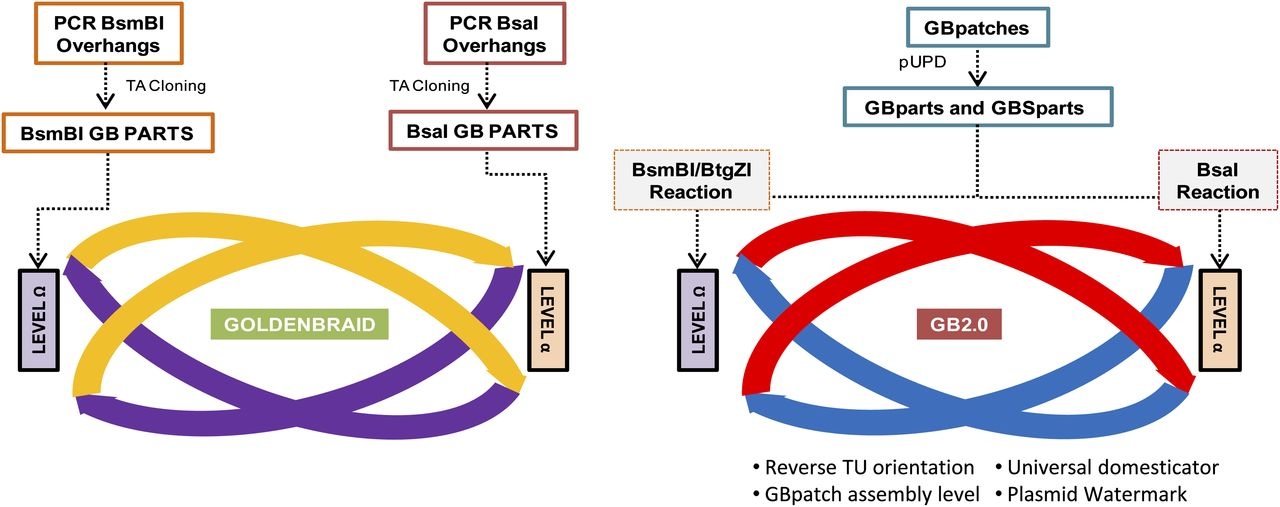
\includegraphics[width=\textwidth]{images/chap4/chap4_gb_01.png}
    \label{fig:ch4gb01}
\end{figure}
\FloatBarrier
\noindent
After building a new TU , utilizing a multipartite assembly, the resulting new transcriptional unit can be binarily combined with another transcriptional unit to produce increasingly complex multigene structures. The solution provided by GoldenBraid cloning system relies on the special design of GoldenBraid destination vectors, which introduces a double loop (braid) into the cloning strategy. A composite part (a TU or a group of TUs) cloned in a given entry vector can be combined only with a second composite part cloned in the complementary entry vectors at the same level. This is done in the presence of a destination vector of the opposite level and generates a new expression vector at the opposite level. \\ \\
Besides the most adapted Modular Cloning system, the Golden Braid system is also adapted in the plant synthetic biology community. After the introduction of the Phytobrick standard, both standards became compatible and accelerated the characterization of standardized genetic parts for plant engineering \parencite{Sarrion-Perdigones2013}.


% =====================================================================
% ============================== CHAPTER ==============================
% =====================================================================

\chapter{Standardization}

\section{Measurement}
\epigraph{The following chapter was written by Michael Burgis}{\textit{iGEM Marburg 2021}}
\noindent
With this chapter we would like to describe good practice for the test phase during an iGEM project and what aspects need to be especially taken into consideration when working with phototrophic organisms.
\\ \\
In synthetic biology, measurement refers to the process of testing and characterising a system or device. Good measurement ensures that the data you produce is relevant, comparable, accurate, reliable, and reproducible.
To ensure the collected data to fulfill all of these requirements a lot of planning and supporting experiments need to be designed.
\\ \\
Most of the data generated by the iGEM teams tends to be collected during the end of the project. Therefore it is of high priority to work out potential problems and the general design of the measurements that are to be conducted as soon as possible. As a useful resource, iGEM itself already offers a helpful question catalog about which aspects you may consider before planning your experiments. This catalog can be found following this website \\ \href{https://2021.igem.org/Engineering/Test}{https://2021.igem.org/Engineering/Test} under the section \textbf{Question to consider for wet lab projects}.
In addition, it is very important to plan how to address the identified problems.
\\ \\
While the aforementioned link also includes resources like the description to use iGEM-provided standards or measurement protocols, they are mainly targeted to the well established lab chassis \textit{E.coli} and are only partially suited for phototrophs making the generation of quantitative data comparably harder.
\\ \\
Chlorophyll and other autofluorescent molecules present in phototrophs can present quite some troubles considering optical density and fluorescence measurements. 
For OD measurements it is important to know the absorption spectrum of your organism of choice and then choose the wavelength accordingly. The measurement of microalgal and bacterial cultures using a photometer or a plate reader is generally done through measuring the turbidity of the cell suspension. This is done indirectly by evaluating how much of the emitted laser is being deflected by the cell suspension. As a consequence, the wavelength should be chosen where the absorption of the organism is relatively negligible. For cyanobacteria and algal cells, 730nm is the most common wavelength setting \parencite{Crozet2018} \parencite{Niederholtmeyer2010} \parencite{Yu2015} \parencite{Wlodarczyk2020} \parencite{Kachel2020}.
\\ \\
Fluorescent reporters are well established in the field of molecular biology. They can be used in plants, algaes and cyanobacteria alike and can be used to characterize genetic parts. Similar to OD measurement, fluorescence measurements are affected by autofluorescence. Due to major peaks of autofluorescence emission in the blue to green \parencite{Rasala2013} and the far red range \parencite{Kavna2009}, we mainly advise to use reporters that emit in the yellow to red range.
The website \href{https://www.fpbase.org/}{fpbase} is a good tool to find a suitable reporter for your project. They offer a database of 784 fluorescent proteins and for most of these proteins accurate excitation and emission spectra are available.


\begin{table} [!htpb]
\centering
\resizebox{\linewidth}{!}{%
\begin{tabular}{|lllllllll|} 
\hline
\begin{tabular}[c]{@{}l@{}}\textbf{Fluorescent}\\\textbf{protein}\end{tabular} & \textbf{Excitation λ}~ & \textbf{Emission λ}   & \begin{tabular}[c]{@{}l@{}}\textbf{Extinction}\\\textbf{coefficient}\end{tabular} & \begin{tabular}[c]{@{}l@{}}\textbf{Quantum}\\\textbf{Yield}\end{tabular} & \textbf{Brightness}     & \textbf{pKa}          & \begin{tabular}[c]{@{}l@{}}\textbf{Maturation}\\\textbf{time (min)}\end{tabular} & \textbf{Lifetime (ns)}  \\ 
\hline
\textbf{LanYFP}                                                                & \textbf{513}           & \textbf{524}          & \textbf{150.000}                                                                  & \textbf{\textbf{0.95}}                                                   & \textbf{\textbf{142.5}} & \textbf{\textbf{3.4}} & -                                                                                & -                       \\ 
\hline
\textbf{mScarlet}                                                              & \textbf{569}           & \textbf{\textbf{594}} & \textbf{\textbf{100.000}}                                                         & \textbf{\textbf{0.7}}                                                    & \textbf{\textbf{70}}    & \textbf{\textbf{5.3}} & \textbf{\textbf{174}}                                                            & \textbf{\textbf{3.9}}   \\
\hline
\end{tabular}
}
\end{table}
\FloatBarrier
\noindent
A possibility to avoid this background fluorescence is by switching to bioluminescent reporters. These enzymes can catalyze reactions for specific substrates and in turn produce a light signal that can be detected by an analytical device of choice. The signal from this reaction is generally high and shows low background making it a suitable reporter for phototrophs. But due to its mechanism it is only possible to perform end point measurements.
\\ \\
Besides these usual reporter genes, we can recommend a recently published reporter system based on plant pigments called RUBY \parencite{He2020}. It is based on the betalains that can be used for quantitative measurements using photometric measurements. This system consists of the three enzymes needed to convert tyrosine to betalains. In RUBY, they are combined in one single open reading frame and separated by 2A peptides, which can later separate the proteins by self-cleavage. So, the three enzymes are transcribed and translated together. In the end, the three individual enzymes are released and are completely functional. 
\\ \\
Plate readers and other equipment using photometrics in order to measure samples are not usable for the generation of comparable data. Every lab has different equipment with different settings, and measurements of fluorescence or absorbance from this equipment are often reported using arbitrary units (AU). These AU values from different labs cannot be directly compared, which hinders reproducibility and can discourage others from building on your work and/or using your systems.
\\ \\
Measurement standards can be used to calibrate equipment and convert arbitrary units to absolute units, which are comparable. In the past the iGEM foundation usually included these standards in their distribution package. These standards included fluorescein, which can be used to convert arbitrary units of fluorescence to values equivalent to a molecule of fluorescein \parencite{Beal2018}. Also, a standard for the conversion of OD to special silica beads was included in order to better quantify the amount of \textit{E.coli} cells in a sample \parencite{Beal2020}. While the fluorescein normalization can be done for phototrophs as well, the silica bead normalization depends on the size of the organism. Therefore it should be possible to convert arbitrary OD measurements for phototrophs using silica beads with the right size. Unfortunately, no standard for luminescent reporters has been established making it impossible to quantitatively compare luminescent data across laboratories.




\section{Normalization}
Although there are a lot of external factors that can be standardized for more reproducible plant growth and data generation, some biological processes simply cannot be standardized.
\\ \\
In order to generate more reproducible data using phototrophs we propose to use a dual reporter system. The idea is to always include a gene cassette in every construct  that stays the same. This allows us to statistically normalize to it and eliminate variation between measurements. This way it is possible to produce more comparable data across different experiments. In literature this system was successfully used in protoplasts of \textit{Arabidopsis thaliana} and \textit{Sorghum bicolor} and compared to actual stable transformants \parencite{Schaumberg2015}.
\\ \\
This system can be used in conjunction with fluorescent reporters as well as luminescent reporters. For fluorescence we advise to use the two proteins we mentioned in the last chapter. Their difference in the emission maxima makes it possible to use the two peptides and measure them in one run without too much background signal by choosing the excitation wavelength accordingly.
\\ \\
For luminescence we advise to use commercial dual luciferase kits. These kits usually lyse the cell material and subsequently measure the reporters in the same reaction mixture. This is achieved by quenching the signal of the first luciferase. On the one hand these systems are very sensitive and exhibit low background signal, but on the other hand these systems are very costly and are not suited for time series data generation.



% =====================================================================
% ============================== CHAPTER ==============================
% =====================================================================

\chapter{Biosafety}

\section{Cartagena Protocol and Biosafety Resources}
\epigraph{The following chapter was written by Lidia Bobrovnikova \& Ilya Rubinstein}{\textit{iGEM LMSU 2021}}
\noindent
Living modified organism (LMO) is literally any organism whose genome was changed in any way. There is a great variety of higher plants which appear to be LMO, e.g. maize, cotton, soya beans, etc. \\
The concept of biosafety encompasses a range of measures, policies and procedures for minimizing potential risks that biotechnology may pose to the environment and human health. Establishing credible and effective safeguards for GMOs is critical for maximizing the benefits of biotechnology while minimizing its risks. Such safeguards must be put in place now, while biotechnology is still relatively young. 

\subsection{BCH}
After the foundation of Cartagena protocol more people became more aware of biosafety while handling organisms. This caused the development of databases for further research. The most popular platform today is \href{https://bch.cbd.int/protocol/text/}{BCH}, where most biosafety protocols are published. There can also be found the geography, ancestors, toxicity, composition, history of modifications etc. of any strains and cell cultures around the globe. 

\subsection{IPPC}
\href{https://www.ippc.int}{IPCC (international plant protection convention)} is responsible for tracking the appearance of transgenic plants, preservation of the primary species, etc. 
 

\section{Plant Biosafety Levels}
There are four biosafety levels and associated practices for plant research. Only BSL-1P and BSL-2P research is conducted at the UW. There are no BL3-P or BL4-P experiments at the UW. 
\subsection{BSL-1P}
BSL-1P is recommended for transgenic plants that are not noxious weeds, are not easily disseminated and are not detrimental to the environment.\\ 
Requirements at BSL-1P include:
\begin{itemize}
    \item Access to the laboratory and greenhouse is limited or restricted when experiments are in progress.
    \item Prior to entering the greenhouse, personnel are required to read and follow instructions on BSL-1P greenhouse practices and procedures.
    \item All procedures must be performed in accordance with accepted greenhouse practices appropriate to the experimental organism.
    \item Records will be kept of experiments currently in progress in the greenhouse facility.
    \item Render experimental organisms biologically inactive by appropriate methods before disposal.
    \item A program shall be implemented to control undesired species (e.g., weed, rodent, or arthropod pests and pathogens) by methods appropriate to the organisms and in accordance with applicable state and federal laws.
    \item House arthropods and other motile macroorganisms in appropriate cages. If macroorganisms (e.g., flying arthropods or nematodes) are released within the greenhouse, precautions must be taken to minimize escape from the greenhouse facility.
    \item The greenhouse floor may be composed of gravel or other porous material. Impervious (e.g., concrete) walkways are recommended.
    \item Windows and other openings in the walls and roof of the laboratory and greenhouse facility may be open for ventilation as needed for proper operation and do not require any special barrier to contain or exclude pollen, microorganisms, or small flying animals (e.g., arthropods and birds). Screens are recommended.
    \item Laboratories and greenhouses must be locked when unoccupied. All agents must be secured against accidental exposure, unauthorized use, and theft. All recombinant nucleic acids must be stored in locked containers.
\end{itemize}
\subsection{BSL-2P}
BSL-2P is recommended for transgenic plants that are noxious weeds or can interbreed with noxious weeds, transgenic plants that contain the genome of an non-exotic infectious agent, and transgenic plants or plant pathogens that may have a detrimental impact to the environment.
The following are required when working at BSL-2P:
\begin{itemize}
    \item A program to control undesired species (e.g., weed, rodent, or arthropod pests and pathogens) by methods appropriate to the organisms and in accordance with applicable state and Federal laws.
    \item A greenhouse floor composed of an impervious material. Concrete is recommended, but gravel or other porous material under benches is acceptable unless propagates of experimental organisms are readily disseminated through soil. Soil beds are acceptable unless propagates of experimental organisms are readily disseminated through soil.
    \item Materials containing experimental microorganisms must be transferred in a closed , leak proof container.
    \item An autoclave must be available for the treatment of contaminated plant material including soil.
    \item If intake fans are used, measures shall be taken to minimize the ingress of arthropods. Louvers or fans shall be constructed such that they can only be opened when the fan is in operation.
    \item Greenhouse containment requirements may be satisfied by using a growth chamber or growth room within a building provided that the external physical structure limits access and escape of microorganisms and macroorganisms in a manner that satisfies the intent of the foregoing clauses
    \item Laboratories and greenhouses must be locked when unoccupied.
    \item All agents must be secured against accidental exposure, unauthorized use, and theft.
    \item All recombinant nucleic acids and BSL-2P agents must be stored in locked containers.
    \item All material in the open bay or common use areas must be secured when not in use.
\end{itemize}
\subsection{Plant Containment and Handling} 
Plant containment can be physical or biological. Physical containment can include a plant growth chamber or a greenhouse, whereas biological containment refers to removal or inactivation of plant reproductive structures (pollen and seed). Methods to contain or handle plants may include:
\begin{itemize}
    \item Facilities such as research labs, growth rooms, or greenhouses
    \item Procedures, practices, and personal protective equipment (PPE)
    \item Transportation and storage
\end{itemize}
For transgenic plant research, standard operating procedures (SOPs) that describe methods to contain plants, associated organisms and waste are required.
\href{https://www.ehs.washington.edu/biological/biological-research-approval}{Biological Use Authorization (BUA)} is required for all plant research involving recombinant or synthetic nucleic acids (DNA/RNA).
Regulations governing plant research depend on the type of research, and whether plants, plant pathogens, plant-associated arthropods, noxious weeds, invasive plants, or other biological agents are used.
\href{http://www.aphis.usda.gov/aphis/resources/permits}{APHIS permits} may be required.

\subsection{Field Work} 
Field work with transgenic plants requires permits from APHIS prior to the start of work. If you have any plans to do field work with genetically engineered plants or associated organisms, inquire about permits first.
\subsection{Biohazardous Plant Waste}
Plant waste, including all transgenic plants, seeds, spores, plant debris and soil materials, and any plants exposed to plant pathogens are considered biohazardous waste and must be inactivated prior to disposal. Refer to \href{https://www.ehs.washington.edu/biological/biohazardous-waste}{Biohazardous Waste} for more information on methods of decontamination and disposal.

\section{Edible Microalgae}
Microalgae have a significant potential as a food source. Their biomass contains a great amount of essential for human compounds (unsaturated fatty acids, amino acids, vitamins, flavonoids etc.). Moreover, production of microalgae is economically sustainable. However, today the price for microalgae biomass suitable for nutrition is quite high, though it can be curtailed if production is moved to a greater scale. 
Nowadays, the most popular species of microalgae for food are \textit{Spirulina} (\textit{Arthrospira sp.}) and \textit{Chlorella sp.} Both these organisms are used today as a food additive in animal and human diet. They produce all essential amino acids, most vitamins and essential unsaturated fatty acids. Interesting to note, that their biomass is richer in protein than soybeans. \\
Overall, microalgae contain a great variety of organic compounds: volatile compounds, sterols, proteins, all classes of lipids and polysaccharides etc. However, some compounds, especially volatile and phenolic compounds, can be hazardous \parencite{Andrade2018} \parencite{Torres-Tiji2020}.

\section{Toxins of Microalgae and Cyanobacteria}
Some microalgae are able to produce by-products or as “waste” molecules some toxic compounds. The most popular classes of such toxins are neurotoxins and hepatotoxins. 

\subsection{Hepatotoxins (Microcystins, Nodularines)}
These molecules have a particular for this class of toxins mechanism of action and biosynthesis. They can cause such symptoms as high temperature, diarrhea and indisposition. These molecules are not commonly produced by cyanobacteria and their synthesis is initiated with the separation of cells in the colony. This can be avoided when using heating and MV of cultures.

\subsection{Neurotoxins (Anatoxins, Saxitoxins)}
This class is characterised by numerous mechanisms of action and different molecule stability. \\ 
Anatoxins are less hazardous for human, however, may cause lethality. These molecules are quite stable, but can be broken down by cyanobacteria themselves after a long period of storing of culture in non-sterile conditions. 
Saxitoxins are probably ones of the most hazardous of the known substances. Their action is slighter than in anatoxins, but their stability is much greater and they can be synthesized \textit{in vitro}.  These toxins are produced by dinoflagellates and diatoms and there are quite a lot of cases of poisoning (red tides — harmful algal blooms) \parencite{Yunes2019} \parencite{Sivonen2009}. 

\section{Catastrophes caused by Plants, Algae and Cyanobacteria}
\subsection{Water Blooms}
Algae blooms are an increase of algae number in the water. This phenomena can be seasonal or spontaneous. Seasonal blooms are often caused by prolonging the day, increasing the temperature and oxygen concentration near the water layer. These blooms are not dangerous for ecosystems and do not cause catastrophes due to the variation of different species with different toxins in the water. \\
In contrast, spontaneous blooms are more noxious for ecosystems. There are a few reasons for that, but the most popular explanation is eutrophication — an excess of  biogenic compounds in the water. Eutrophication can be both natural and caused by humans. A rapid increase of nutrients of water causes a massive propagation of algae and, subsequently, a critical accumulation of dissolved oxygen and growth of toxic compounds concentration produced by algae. Finally, the complex of aforementioned reasons is followed by an extinction of water animals. \\
Water blooms can be circumvented by following the rules of national and specific communities and making an analysis of water conditions. 

\subsection{Invasive Plants}
It is common knowledge that many plants are able to adapt to new conditions and repress the indigenous species by bringing changes into ecosystem hierarchy. \\
One such example is \textit{Elodea canadensis}. Initially this species comes from North America, but today it is spread to Europe, Asia and Africa. This species has a very high growth rate and ability to survive in rapidly changing conditions. 
How can we prevent the contamination of ecosystems with invasive species? Thinking as pessimists — there is no way. This is a natural process of spreading species. A new challenge for scientists!


% =====================================================================
% ============================== CHAPTER ==============================
% =====================================================================

\chapter{Metabolic Engineering}

\epigraph{The following chapter was written by the MADRID Team }{\textit{iGEM Madrid\_UCM 2021}}
\section{What is Metabolic Engineering}
Metabolic Engineering (ME) consists in the directed modification and regulation of an organism' metabolic pathways for metabolite over production or the improvement of certain cellular features. Either native pathway engineering, introduction of heterologous pathways or the design of synthetic pathways for converting microorganisms into microbial cell factories can be considered Metabolic Engineering applications. \\ \\
The field of Metabolic Engineering is highly interdisciplinary being closely related with synthetic biology. Metabolic engineering is a complex task which requires the elucidation of existing or novel metabolic pathways, their manipulation and regulation by gene edition techniques as well as efficient probing systems for the implemented metabolic pathways. Then, the application of appropriate methods from molecular biology, along with techniques from engineering  such as modeling and data analysis are a key feature of metabolic engineering. \\ \\
Recently Metabolic Engineering field is evolving towards a systems  biology approach, leading to outstanding advances in strain engineering. Systems Metabolic Engineering aims to speed up the pathway prototyping process and its scale up to industrial processes. In fact, Metabolic Engineering is currently evolving into a novel manufacturing technology where either computational and mathematical analysis are being combined with experimental approaches for rational engineering of microorganisms. Currently, these tools are fueling the development of a new area, where metabolic engineering principles can be even applied in-vitro, where metabolic pathways occurs and regulate completely outside of any organism \parencite{Wei2020}.
\\ \\
\section{Key Notions in Metabolic Engineering}
It is common to observe how allegedly well-designed heterologous pathways experience low yields when implemented into a different organism. There are several reasons for this to happen. Adequate regulation of the pathway is either crucial and a challenging task, which vastly depends on the chassis organism and the availability of well characterized genetic elements. \\ \\
However, the first step for metabolic engineering is to elucidate how a pathway should be regulated, and despite Metabolic Engineering can be a really complex work, there exists several rules of thumb that should be considered into any metabolic engineering design. Within this section you will find some of this basic principles that can be applied for pathway optimization and consequently, increasing the productivity of a certain metabolite.
\subsection{Carbon Flux}
Carbon Flux is they cornerstone of Metabolic Engineering. This concept refers to the way carbon is routed towards the more or less intrincated pathway network which comprises an organism metabolism. Carbon Flux refers to the amount of carbon atoms that are routed from the carbon source/s of an organism towards certain metabolic pathways. Depending on the organism and environmental conditions carbon can be partitioned via many different pathways. \\ \\
Essentially carbon flux consists on a concept that allows to weight the importance of certain reactions within a pathway, considering the amount of carbon which is being converted in the organism via that specific reaction/s.  The higher carbon flux is towards certain pathway, higher production of metabolites related from that pathway could be achieved. \\ \\
Carbon Flux concept is crucial since it allows the visualization of an organism metabolism in a very simple perspective. From this perspective, metabolism can be considered as a pipe network, where there are \textbf{carbon sources} where carbon uptake from outer media occurs, and there are \textbf{carbon sinks} where the acquired carbon escapes the metabolism and virtually stops experiencing transformations. \textbf{Carbon sources} are generated by the first \textbf{carbon assimilation reactions} belonging to catabolism, while \textbf{anabolic reactions} leading to the formation of biomass or metabolites that eventually will be secreted creates \textbf{carbon sinks}. \\ \\
Most of metabolic reactions are reversible, this implies that if a carbon sink is close to a pathway, it will “attract“ carbon flux towards its direction, since the final product of the reaction is being “dragged“ displacing the equilibrium towards the final products. Then an useful strategy for re-routing carbon is to create carbon sinks capable of pulling carbon out from the central metabolism towards the desired reactions. \\ \\
Likewise, carbon flux can provide an idea of which pathway can be more optimally implemented within a certain organism just attending to which set of reactions naturally posses a higher carbon flux. Those pathways which has higher carbon flux will provide a more abundant carbon supply for heterologous pathways feeding on them.
\subsection{Metabolite Availability}
Another crucial aspect to consider is the existence of \textbf{key metabolites} and how available they are. Taking into account the former concept of carbon flux, there exists certain metabolites which are central nodes of several pathways. \\ \\
When designing or implementing a pathway within an organism, it is essential to consider which are going to be the native metabolites to be converted into the desired final product. The most abundant a metabolite is, the easier will be for an alternative pathway to efficiently drag carbon via the desired reactions towards the carbon sink that is the final product. \\ \\
Depending on the chassis organism and its metabolic state, certain metabolites would be more abundant than others. Then selecting those metabolites with higher abundance will result in higher productivities in the end of the pathway. \\ \\
As an example, metabolomic analysis has show that certain cyanobacteria such as \textit{Synechocystis sp.} PCC6803 have an acetyl-CoA availability ten times higher during normal growth conditions compared to \textit{Synechococcus sp.} PCC7002. This “baseline concentration“ of a certain metabolites during normal cell growth is defined as “metabolite pool“. \\ \\
Then another strategy to increase the productivity of a certain pathway is not only to start from a central metabolite which is already highly available within the chassis, but also to implement additional reactions in the metabolic design that increase the conversion of other metabolites towards this “key metabolite“.
\subsection{Branching and Competitiveness in Pathway Networks}
Metabolic pathways often do not take place on a linear fashion, but they rely on several interconnections. When implementing a pathway it is crucial to consider all the already existing pathways within the cell and how can they actually drag or supply carbon to the target pathway. \\ \\
Bothe the final and the intermediate subproducts can be potentially transformed via certain pathway already present within the organism. Therefore a key aspect to consider is the existence of competing pathways, capable of dragging carbon from the desired pathway re-routing it back to other native metabolic functions.
\begin{itemize}
    \item[] An \textbf{example} of this is the ability to synthetize energy storage compounds such as Polyhidroxyalkanoates (PHAs) or Polyhydroxybutyrate (PHBs). Certain bacteria express PHA/PHB synthases, capable of synthetizing PHAs or PHBs from acetyl-CoA derived metabolites. Each PHA synthase converts certain acetyl-CoA derived metabolite (Acetyl-CoA, Acetoacetyl-CoA, R-3-OH-butyryl-CoA, 3-OH-acyl-CoA etc...) into another key metabolite required for the PHA/PHB synthesis pathway.
 
    \item[] When implementing  a pathway which starts from acetyl-CoA as key metabolite, or some of its steps involves the formation of this acetyl-CoA metabolites, considering if the chassis organism is capable of synthetizing PHAs/PHBs or not could be crucial. In PHAs/PHBs synthetizing organisms, the overproduction of some of this intermediate metabolites via the introduced pathway could trigger the synthesis of PHAs/PHBs, reducing the pathway yield or even completely numbing  the formation of the final product. Then, a knock out of this PHAs/PHBs synthase genes will be desirable to enhance pathway productivity. In the other hand, if the chassis organism is not a natural producer of PHAs/PHBs, the pathway could be implemented without further problems, and the intermediate metabolites will mainly be directly channelized towards the final product.
\end{itemize}
Most of this competing pathways are usually found in the early stages of a pathway, where a certain key metabolite is converted into the intermediate precursors of the final product. Key metabolites usually act as a branching point for carbon flux. When possible, usually down-regulating or knocking-down non-essential pathways feeding on the key metabolite is a good strategy for increasing the carbon flux towards the desired pathway.
\subsection{Metabolic Burden and Metabolite Toxicity}
Eventually, one crucial aspect when engineering the metabolism of an organism is the potential toxicity that the introduction of genetic modifications can produce. This toxicity can mainly develop via two different reasons: excessive metabolic burden of the pathway or inherit toxicity of the final product or intermediate metabolites.

\subsubsection{Metabolic Burden}
Most of the pathways start from a very few key metabolites. This leads to a situation where it is common to observe how artificial metabolic pathways suffer from low productivity because carbon is usually preferentially routed towards the native pathways. A common strategy to overcome this issue is to up-regulate the expression of the foreign pathway (codon optimization, use of strong regulatory elements etc). However, the usage of too strong promoters or RBS can lead to impaired cell growth or even cell death. When the expression of a pathway is so high that it comprise even the basic metabolic functions, the metabolic burden of that pathway is high. \\ \\
Metabolic burden can be defined the proportion of the resources of a host cell that are used to operate the artificially introduced or modified pathways  within a host cell. Cell resources can be either energy (ATP and cofactors) or carbon molecules used as building blocks. Consequently, when implementing a pathway in a specific chassis organism, it is crucial to consider what would be the metabolic burden that the pathway and its regulation will impose to the organism.
 
\subsubsection{Metabolite Toxicity}
 
Likewise, some metabolites are toxic to the cells. When a pathway is overexpressed and huge amounts of certain compounds start accumulating in the cell, the toxic effects of the metabolites start becoming stronger till the cells eventually die. Depending on the biochemical nature of the synthetized compounds, toxicity may arise from many different mechanisms. However, in any of this cases, the implementation of supporting genetic modifications, able to relieve the cells from the toxicity of the product, is a common strategy to increase the pathway productivity.
\begin{itemize}
    \item[] An \textbf{example} of this is the production of biofuels using microorganisms. Most of biofuels are lipophilic or at least the molecule harbors a lipophilic region. This feature of the final product and some of its intermedium metabolites generate cell toxicity via the interaction with cell membranes
    \item[]It is common to observe that microorganisms modified only for the overproduction of free fatty acids, fatty acids methyl esters, short to medium chain alcohols, alkanes or isoprenoids (all of them promising biofuel candidates) usually suffer from impaired cell growth and moderate yields. When cultures grow for long periods of time, accumulation of desired products starts to plateau as a consequence of the toxicity of the product.
    \item[]Among the common strategies to overcome this problems are the selection of robust chassis organisms with native mechanisms for solvent tolerance like yeasts or the implementation of secretion mechanisms for pumping out the toxic products from the interior of the cells.
\end{itemize}

\subsection{Pathway Design}
\textit{Metabolic Engineering} relies either in the optimization of already existing pathways and its adaptation to other heterologous chassis and the design and implementation of \textit{de novo} artificially designed pathways. Currently the field of \textit{metabolic engineering} is evolving fast towards the computer-aided design of pathways at the genomic level, taking into account all the potential interactions between the already-existing pathways of a chassis organism, and the possible reaction schemes that could be implemented to achieve specific goals. \\ \\
Despite the aim of this chapter is not to provide a deep insight within how to design metabolic pathways but establish the guidelines for smart pathway design, it is important to remark the existence of several tools for pathway design and optimization. To know more about, Otero-Muras \& Carbonell covered extensively this topics in the review article cited in the references.
\section{Phototrophs Metabolic Engineering}
An heterotrophic organism such as \textit{S. cerevisiae} feeding on sugars will route most of the carbon towards the glycolysis pathway and after that carbon flux will start branching in different routes. Part of it will be derived towards the energy metabolism, becoming CO2 or ethanol, while other part of the carbon flux will be redirected to anabolism becoming part of the cell constituents or secondary metabolites used for defense or communication. In short, heterotrophic metabolism uses organic compounds as both carbon and energy sources. \\ \\
On the other hand a phototrophic organism route most of the carbon towards the Calvin–Benson–Bassham (CBB) cycle or similar carbon fixation pathways. CO2 and the solubilized HCO3- are used as the main carbon sources, while the energy comes from the environmental light. In a phototrophic organism, energy is harvested during the light step of the photosynthesis, while carbon is captured during the dark phase of the photosynthetic process. A deep comprehension of this aspects is essential to truly understand phototrophic metabolism.
\subsection{Phototrophic Organisms and Phototrophic Metabolism}
Phototrophic metabolism widely differs from the conventional heterotrophic systems. Despite the huge differences among the different phototrophic metabolism there exists certain features that phototrophic organism share and makes them different from other standard chassis in synthetic biology. \\ \\
In addition, it is important to remark that the availability of well characterized regulatory elements, standardized protocols, measurement methods and metabolic models for phototrophs still long way behind all the tools available for heterotrophs. \\ \\
One key aspect is the \textbf{cofactor abundance (NADPH / NADH ratio)}. In heterotrophs NADH is the main cofactor, produced during the energy metabolism and mainly used for catabolic pathways. Meanwhile NADPH is mainly employed for anabolism and obtained via the interconversion of formerly generated reducing power. In phototrophs NADPH is the principal cofactor generated during photosynthesis and the NADPH pool is much more abundant than the NADH one. This is a common characteristic of phototrophs and one of the reasons why heterologous pathways coming from heterotrophs usually display poor yields when cloned into phototrophic chassis. \\ \\
Another important aspects and differences between the principal phototrophic chassis are detailed in the table below:

\begin{figure}[!htpb]
    \centering
    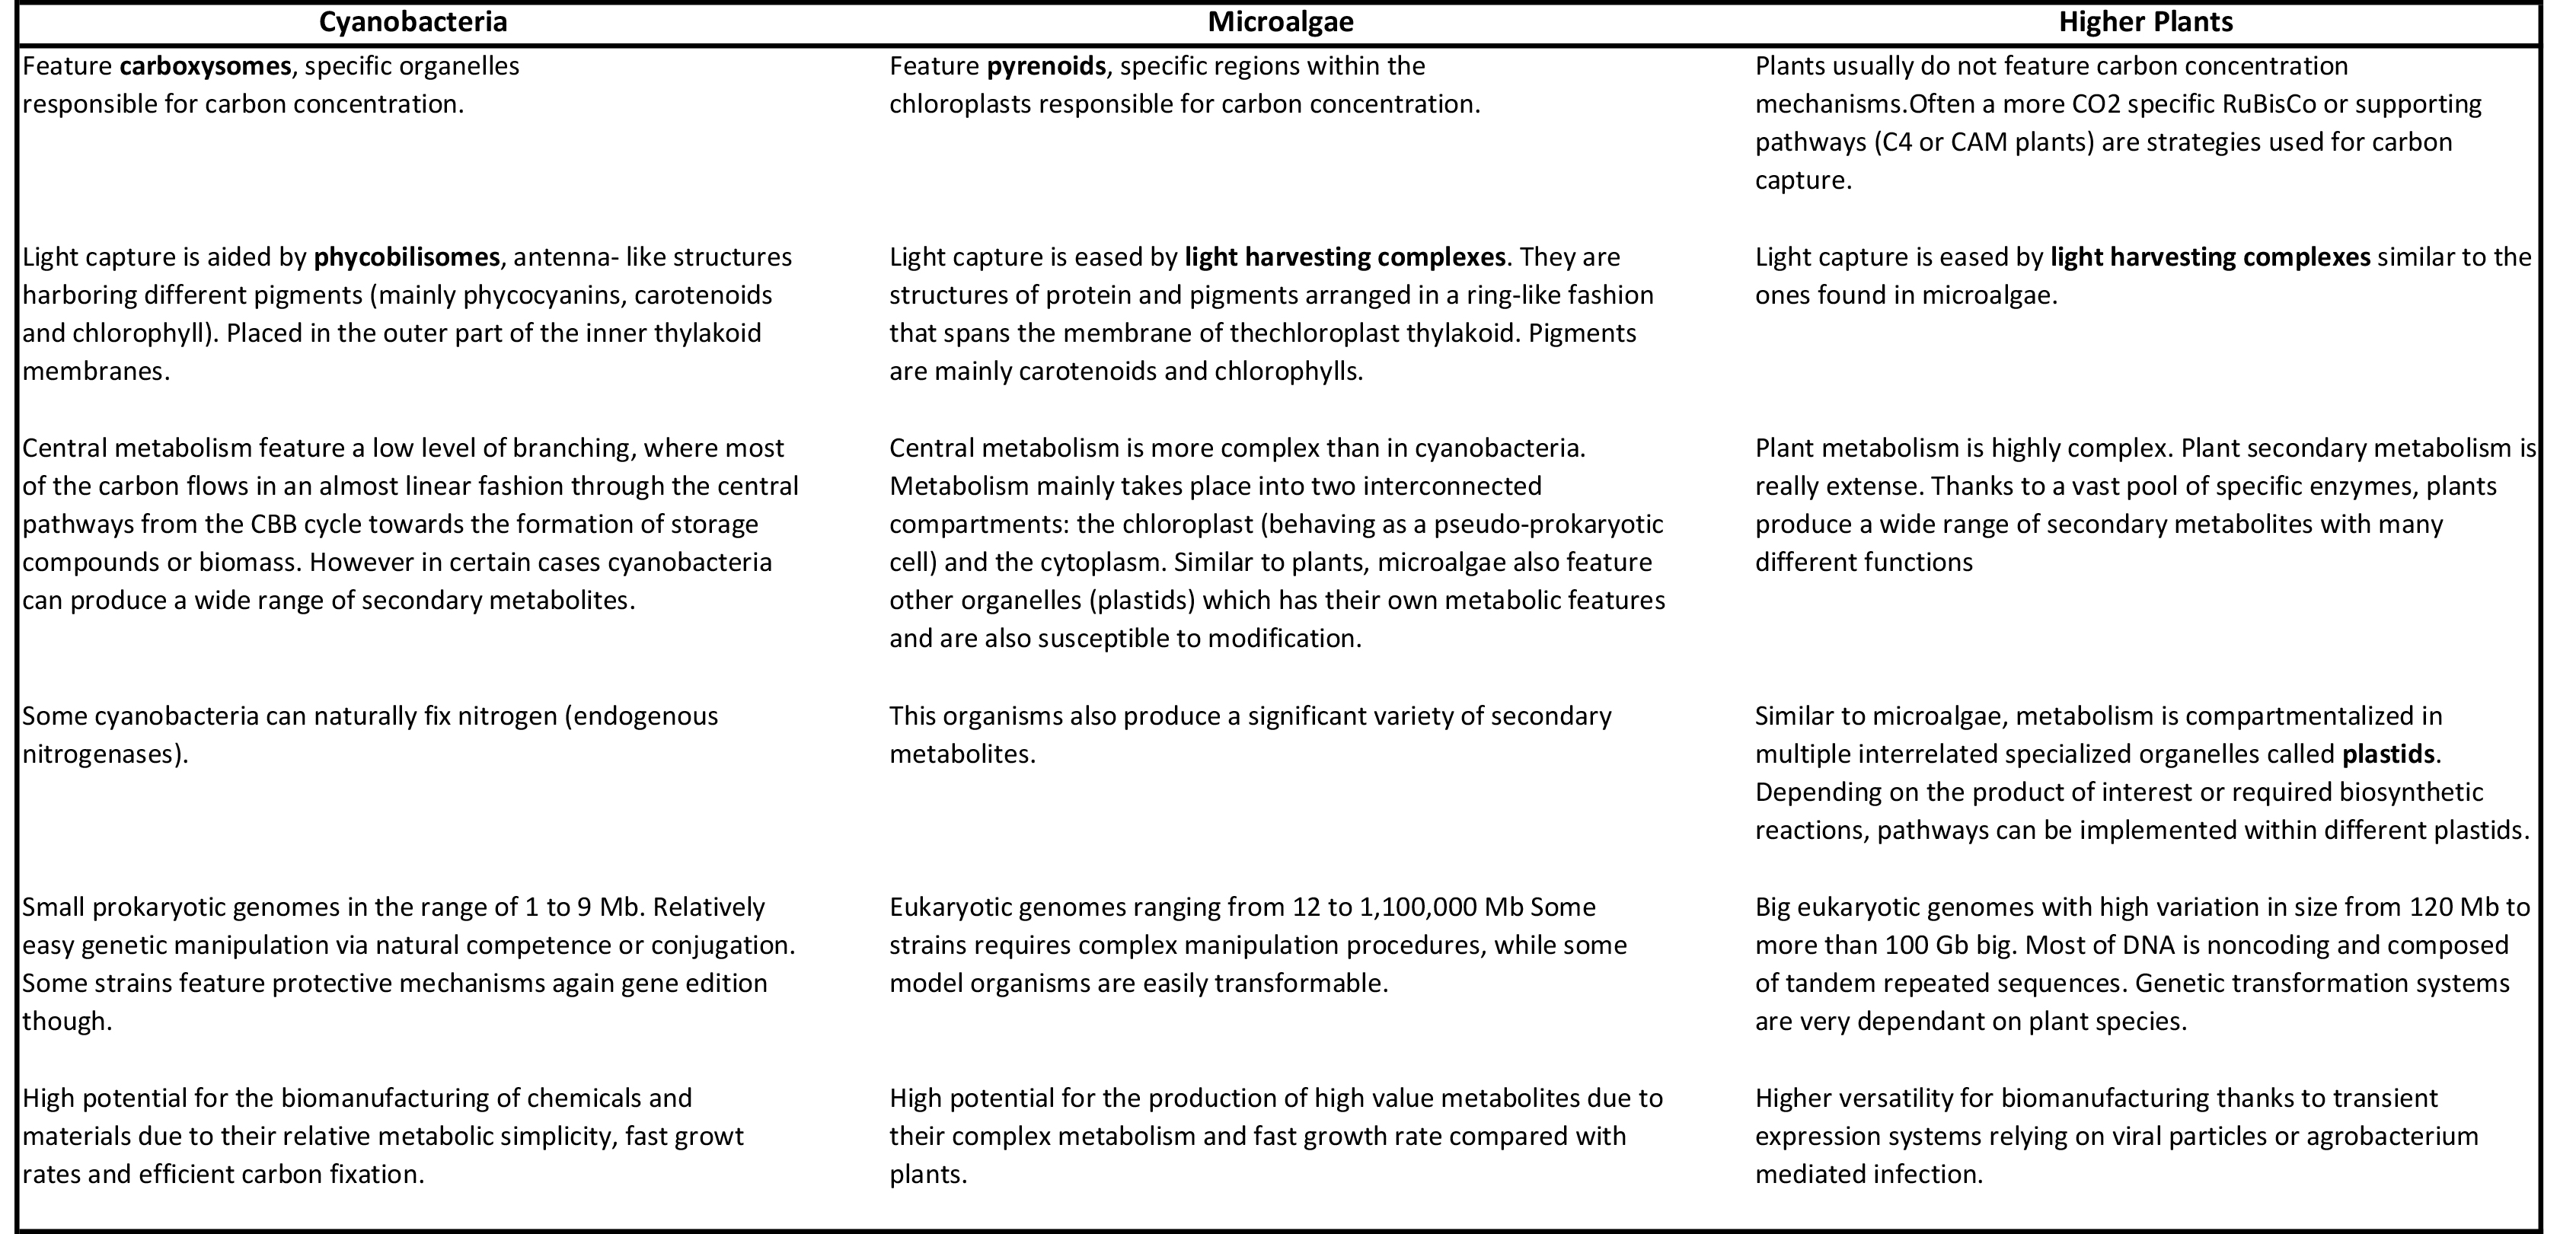
\includegraphics[angle=-90, scale=0.2]{images/chap7/table_met_eng.jpg}
    \label{fig:chp7landscapetable}
\end{figure}
\FloatBarrier
\noindent
Briefly, it is important to consider that phototrophic metabolism is different from heterotrophic organism. Thus metabolic engineering of phototrophs will require specific considerations and design rules that could differ to the ones applied in heterotrophs. \\ \\
All the formerly introduced concepts still applying for metabolic engineering of phototrophs. However, there are some key aspects that must be taken into account to efficiently engineer the metabolism of phototrophic organisms and harness their full potential as photosynthetic bio-factories. \\ \\
The subsequent sections will provide a brief insight within the strategies that can be implemented within a phototrophic chassis in order to enhance the productivity of metabolic pathways.
\subsection{Strategies to Enhance Carbon Fixation}
While heterotrophs rely on the availability of different carbon sources, phototrophs depens on an unique substrate: Carbon Dioxide (CO2). CO2 or its solubilized form (HCO3-) is the source of all phototrophic metabolism. Then enhancing the ability of an organism to fix carbon and pump it through its metabolism is the first step to optimize the productivity of any pathway. The highest input carbon flux the metabolic network has, the higher availability of carbon will be for any reaction. This way, several strategies can be implemented in order to maximize the carbon fixation.
 \begin{itemize}
     \item[] \textbf{RuBisCO engineering}. Ribulose-1,5-bisphosphate carboxylase-oxygenase or RuBisCO is the enzyme responsible for carbon fixation in almost any photoautotrophic organism. However RuBisCO is rather inefficient and high amounts of the enzyme are produced in order to allow the cells fix enough carbon for their survival. Likewise, RuBisCo can catalyze the oxidation of Ribulose-1,5-bisphosphate, producing 2-phosphoglycolate, a toxic metabolite that must be recycled via the photorespiratory metabolism, loosing carbon and spending energy.
     \item[] To avoid the photorespiration drawbacks each organism has evolved their own version of RuBisCO variants. RuBisCO in cyanobacteria is highly active and efficiently catalyzes carbon fixation. However its selectivity towards CO2 is poor. On the other hand, plant RuBisCO is less active than the cyanobacterial counterparts (even 3 times less active), but the selectivity towards CO2 is up to twice higher.
    \item[] Depending on the chassis organism and desired conditions for the organism development, the introduction of heterologous or engineered RuBisCO variants can be a strategy for improved carbon fixation. However, despite RuBisCO engineering has been attempted several occasions, most of the published bibliography demonstrates that only moderate improvements can be achieved, and most of the time selectivity should be compromised in favour of activity or vice-versa.
 
\item[] \textbf{Reducing carbon loss}.  Photorespiration as well as other pathways reduces the overall capacity of an organism to assimilate carbon from CO2. Certain metabolic pathways can release carbon molecules as CO2, HCO3-, but photorespiration still being the main process responsible for carbon and energy loss. Photorespiration can lead to a reduction of up to 30\% of the overall metabolic capacity of the organism. Some recent studies has shown the potential role of RuBisCO oxygenase activity in nitrite assimilation and protein synthesis, however photorespiration still being a metabolism branch which can be highly optimized.
    \item[] Several synthetic pathways has been designed in order to reduce the energy expense and carbon losses generated via the photorespiration. Most of this schemes rely on the reconversion of intermediate photorespiration metabolites into the central carbon fixation pathway metabolites.
    \item[] In addition, some artificial pathways has been designed in order to enhance carbon fixation via optimized carbon fixation reactions that could exceed the efficiency of natural pathways such as the CBB cycle.
\item[] \textbf{Carbon Concentration Mechanisms}. Many phototrophs feature specializations that allows them to fix carbon more efficiently. The most common strategy is to increase the CO2 concentration in the cellular compartments where RuBisCO is expressed, this strategies are defined as Carbon Concentration Mechanisms (CCM).
    \item[] An example of CCMs are carboxysomes. Carboxysomes are a cyanobacteria-specific CCM in order to cope with the lower selectivity of their RuBisCO variants. Initially the cell firstly generates a high intracellular bicarbonate (HCO3−) pool through action of membrane inorganic carbon transporters and CO2-converting complexes. This bicarbonate will subsequently be reconverted into CO2 in the carboxysomes to enhance carbon fixation.
    \item[] Carboxysomes are pseudo-organelles composed of polyhedral protein forming a capsid. This capsid is thighly assembled, generating an environment where gaseous CO2 diffusion is impeded. Within the capsid structure carbonic anhydrase (which converts the soluble HCO3- into CO2) , and RuBisCO  are embedded. This way, within the carboxysome CO2 concentration is between 10 to 100 times higher than the external concentration, increasing RuBisCO activity and promoting the selectivity of the catalysis towards carboxylation.
Microalgae feature their own CCMs, while only certain plants have evolved specific adaptations such as the C4 or CAM plants specific carbon concentration mechanisms. In general, every CCM consist on the compartmentalization of carbon fixation reactions in specific environments, where RuBisCO is exposed to higher concentrations of CO2 and lower O2 concentrations, promoting carbon fixation. \\ \\
Either natural or artificial CCMs can be implemented within a chassis in order to improve their carbon fixation efficiency. As an example, some authors have demonstrated an improvement on plant growth rates when cyanobacterial carboxysomes were expressed in the plant chloroplast.
\end{itemize}

\subsection{Strategies to Enhance Light Harvesting}
All phototrophic organisms rely on their ability to convert light into energy, then, the optimization of the light capture phase of the photosynthetic process will allow to increase the efficiency and performance of engineered photosynthetic organisms. To reach that aim, it is necessary to clearly consider the aim of the improvement, in a way that the modification allows for a better performance of the organisms or engineered system in the conditions of the real application. Depending on the conditions of the final application there can be two main possibilities. Either the optimization for high-performance photosynthesis in controlled or favorable environments , or the optimization for high-resistant organisms, able to perform photosynthesis in harsh conditions. \\ \\
The overall photosynthetic performance currently balances between 0.1-1\% in, in some special cases around 2-4\% for plants. Other phototrophs such as cyanobacteria or microalgae can feature slightly higher efficiencies, however the maximum theoretical value is around 10-13\%. The observed relative inefficiency of photosynthesis is derived mainly from the high number of steps involved in photosynthetic process and numerous energy sinks found across the photosynthetic process. In general, there exist three main factors limiting the photosynthetic process: Light, Temperature and CO2 concentration. Controlling either carbon concentration (as explained formerly) or temperature tolerance (enhancing strains robustness and pathway flexibility) can also improve the metabolic performance. However during this section the focus will be made in enhancing light capture.\\ \\
Considering all the aspects involved in the light-phase, multiple bottlenecks for the photosynthetic process can be found. Those critical steps can be used as key points for enhancing light capture performance.
 
\subsubsection{Light Capture Engineering}
First stages of light capture are physical processes involving fast electron transfer reactions with a quantum background. All phototrophs feature specific structures dedicated to light capture, either the Antenna Complex of plants and microalgae, or the phycobilisomes in cyanobacteria and red algae. The modification of these light harvesting systems can directly alter the efficiency of light light to energy conversion within the initial stages of photosynthesis.
\begin{itemize}
    \item[]  \textbf{Light harvesting systems modification} Optimizing the configuration of antenna or light harvesting complexes according with a defined purpose can increase the overall performance. \\ \\
    For example, in the case of microorganisms which will be grown in suspension, truncated antennas can help, reducing the shading effects in bioreactor settings and enhancing overall light absorption. On bioreactor setup or systems where multiple cells are superposed, it allows to distribute the light absorption more efficiently along all the system.  This way there are less cells over-exposed to light (photoinhibition) and less cells experiencing shading. So that, a higher light-stress tolerance and smaller light-to-heat dissipation is achieved. On the other hand higher and pigment-enriched antennas can result in harsh low-light conditions or specific applications.
    \item[] \textbf{Expanding absorbance spectra}. The usage of novel light-absorbing pigments or even different pigments in the reaction centers can enlarge the available light, driving to a higher performance. \\ \\
    As an example, some pigments such as the pigment b-phycoerythrin  of cyanobacteria and red algae feature a light-harvesting efficiency of 98\% compared to the 12\% of pigments found in plants. \\ \\
   Likewise, including different pigments capable of absorbing in other wavelengths , different from the ones that typical light harvesting systems possess can enhance the overall performance of the process. Apart from chlorophyll a, b , carotenoids and similar pigments, there are other pigments that can be used to expand the photosynthetic usable light range.\\ \\
    As an example, most phototrophs can not use light above 700 nm wavelengths. However, some cyanobacteria like \textit{Acaryochloris marina} own a special chlorophyll, able to capture light even in longer wavelengths. It possesses two different chlorophyll molecules:  chlorophyll-d (photosynthetic active center) and chlorophyll-f (light harvesting pigment). That pigments can harvest light at even 760 nm wavelengths. In that organisms, Photosystem I uses Chl.- f, absorbing at 745 nm and Photosystem II is enriched with chlorophyll-f , absorbing at 727 nm. So that, an enhanced usable light spectrum can push the photosynthetic theoretical efficiency from sunlight at a value near 19\%.
 \end{itemize}
However, it is important to consider that although its modifications enhance photosynthetic performance, and grow rates, the modified organisms tend to loose competitiveness against wild-type ones, which has naturally evolved a favorable phenotype. Then rational engineering of light harvesting should always take into account the final application of the engineered organism or system.
 
\subsubsection{Photoprotection Mechanisms}
 
Phototrophic organisms have evolved to adapt to the changing conditions in temperature, irradiance and even CO2 availability. From all of them, light irradiance is the parameter subjected to higher fluctuations. There exists a complex network of different systems that modulate photosynthetic response attending to different changes in the environment. While useful for organism survival, many of these mechanisms lead to energy losses, reducing the efficiency of light-to-energy conversion.\\ \\
These mechanisms widely vary between the organisms, but as general examples are the cyclic electron transfer pathway usually used to balance the ATP/NADPH ration during photosynthesis or the water-to-water cycle, only ATP but no NADPH is produced. That process involves PSII, Cytochrome b6f and PSI. Thos pathways are usually overexpressed during stress conditions, usually during excess reducing power production or excessive photon irradiation. In that condition they dissipate the excess of energy and reduce the generation of highly reactive species that could damage photosynthetic machinery. \\ \\
Some of the strategies that can be followed to enhance light-to-energy conversion are:
\begin{itemize}
    \item[] \textbf{Elimination of energy sinks}. Optimizing the metabolic pathways regulation to avoid entering in cyclic electron flows where the excess of light is not used as energy.
    \item[] \textbf{Relaxing photoprotection systems}. Accelerating the relaxation of energy dissipation an non-photochemical quenching processes can also enhance the overall efficiency.
\end{itemize} 
In general terms, photoprotective mechanisms can widely differ among the different phototrophic chassis. However, altering their pathways in order to reduce the energy sink sizes and modifying the feedback regulation mechanisms to be faster and more precise can also increase overall process efficiency via an useful redirection of the energy surplus produced during intense irradiation periods.  However, these modifications have to be carefully made, to avoid damage in the system, especially when the final usage conditions of the engineered organisms can not be controlled.
 
\subsection{Other Guidelines for Phototrophs Metabolic Engineering}
Eventually, there are some tips and considerations that should be  taken into account when metabolic engineering a phototrophic organism.
\begin{itemize}
\item[] \textbf{NADPH / NADH ration consideration}. When engineering a pathway for a phototrophic organism, certain enzymes would be NADH dependent. In this situation the cellular NADH pool will be crucial for the pathway performance. Avoiding an excessive number of NADH-dependent steps can improve the behaviour of tha pathway. Furthermore the screening for NADPH-dependent enzyme variants with similar activity will be desirable when designing a pathway.
\item[]In the situations where only NADH dependent enzymes feature the desired catalytic function or activity, the implementation of supporting pathways capable of balancing the NADPH / NADH ratio within the organism could be considered. \\ \\
\item[] \textbf{Shorter pathways perform better}. In general, the shorter a pathway is, the more efficient it tends to be. Minimizing the number of reaction steps allows the carbon to flow more efficiently towards the final product, avoiding its loss in competing pathways, or the  reduction in the concentration of the precursor pool into several intermediate metabolites.
\item[] \textbf{Considering the influence of the environment and light cycles}. Most phototrophic organisms feature complex regulatory systems depending on light. As well as other environmental factors, light availability is crucial to determine the metabolic state. Changes in environmental conditions and illumination will produce changes in the metabolism regulation. Among many other aspects, the differential expression of transcription factors can widely alter the central metabolites availability, switch on or off certain native pathways and modify the behaviour of regulatory elements also included within the engineered pathway regulation.
\item[]It is also important to notice that foreign regulatory elements can behave differently within the chassis or even modulate their behavior depending on the cellular state.
\item[] \textbf{Using irreversible reactions as pathway driving-forces}. Most enzymes catalyze reversible reactions, then if a high amount  of a product / intermediate metabolite is produced, the carbon flux across the pathway will be reduced. The introduction of irreversible enzymatic steps (usually addition reactions catalyzed by lyases) , can act as a pathway driving force. Ideally, these irreversible steps should be carefully placed in the critical points of the pathway: in the final conversion step towards the product (avoiding product reconversion) and in the initial pathway steps, where the employed central metabolite could be regenerated.
\item[] \textbf{Codon Usage}. As any other organism, each class of phototrophic organisms will feature a specific codon usage and tRNA availability. Likewise, in cyanobacteria and eukaryotic plasts, it is common to find many open reading frames with alternative start codons such as GTG or TTG. When expressing heterologous genes within phototrophs it is crucial to optimize the codon usage to the classis tRNA availability in order to optimize the transcription process and enhance expression levels.
\end{itemize}
\section*{References}
\parencite{Yadav2018} \parencite{Wuest2011} \parencite{Teng2020} \parencite{Wei2020} \parencite{Tang2011} \parencite{Asplund-Samuelsson2021} \parencite{Jablonsky2016}
\parencite{Otero-Muras2021} \parencite{Zhou2019} \parencite{Shih2016} \parencite{Nielsen2003} \parencite{Wang2017} \parencite{Hanson2016} \parencite{Fang2018} \parencite{Long2018} \parencite{Liang2018} \parencite{Lowe2021} \parencite{South2019} \parencite{Roell2021} \parencite{Xin2014} \parencite{Khurshid2020} \parencite{Basler2016} \parencite{Bloom2018} \parencite{Lea-Smith2016}

% =====================================================================
% ============================== CHAPTER ==============================
% =====================================================================

\chapter{Modelling}

\section{Using computational models for Biological Analysis}
\epigraph{The following chapter was written by members of the University of Miami }{\textit{iGEM MiamiU\_OH 2021}}
\noindent
MATLAB and Python are powerful programs that can be used to manipulate matrices and perform complicated numerical analysis. In the case of synthetic biology, these environments are often used to set up models for biological action, or mathematical representations of complex systems. These mathematical representations can extend to systems with multiple enzymes and interconnected reactions, like the metabolism within the cell. Therefore, through platforms such as MATLAB and Python, we can generate a complex system of inputs and outputs that interact with each other to generate a projection modeling the activity of a system representing a multitude of cells, a single cell, or a microenvironment within a cell. The origin for this method of thinking can be traced back to Boolean circuits, a common mathematical method for combining logic circuits in digital electronic circuits. While these Boolean circuits are useful for projecting basic biological loops, they are not effective to model something as complex as an entire cell through virtual circuits. Instead, a model based on a more complex system of mathematical equations must be used. Dry lab tests using these models allow the team to assess proposed systems or predict outcomes prior to commitment of physical and temporal resources in the wet lab.\\
Although models can be applied to a host of scientific inquiries, due to a primary focus in synthetic and systems biology for phototrophs on using and understanding their metabolic features, this chapter will focus on the analysis of an organism’s metabolism \parencite{Klemencic2017}.

\subsection{COBRA (Constraint-Based Reconstruction and Analysis Toolbox)}
To enable teams to test the impacts of these proposed conditions or added networks on both metabolic reaction fluxes, or rates, and growth of the cells in a dry lab setting, multiple software can be used. However, in this chapter, we will focus on the widely used \href{https://opencobra.github.io/cobratoolbox/stable/index.html}{Constraint-Based Reconstruction and Analysis Toolbox (COBRA)}. A constraint-based model for biochemical networks has a wide range of uses. In the case of analyzing the metabolism of cells, we can input a set of metabolites, reactions, enzymes, kinetic data, and/or stoichiometric coefficients into matrices that are readable by the COBRA Toolbox. Then we input specific constraints to how these inputs can interact that reflect biological limits or desired conditions. From this common set of inputs and constraints, the COBRA Toolbox can present a field of permissible outcomes, in our case fluxes of the different reactions, that allow optimization of a certain condition. This means our team could utilize the toolbox in both MATLAB and Python to generate a host of flux outcomes for any system, or cell with clarified available reaction pathways, that would allow optimization in an area such as production of a metabolite or in growth. This analysis simplifies the temporal and informational demands for the design team as well as provides valuable insight into the feasibility and wet lab parameters for proposed pathways or conditions.

\subsection{Kinetics vs Flux Based Models}
The cell operates via the action of a myriad of enzymatic systems and interactions. From a simple material balance standpoint, mass must be conserved. Our overall system is the cell, and the agents of action are reaction cascades. Within this cell/system, the reaction cascades are observed, and the operators of those cascades are individual enzymatic reactions (4). For these reactions, we have multiple considerations to potentially consider, including thermodynamics, metabolites, enzyme kinetics, mass balances, and enzymatic capacity. All of these are \textit{constraints}, and a model could be defined from a combination of these constraints \parencite{Yasemi2021}.  \\ \\
Reactions are primarily limited by enzymatic kinetics (“speed”) and flux (turnovers of metabolites). Therefore, most models are based on either of these two constraints. Kinetics based models are based on differential equations relating the rates of reactions, taking both kinetics and genetic-based regulation into account. Unfortunately, this model requires enzymatic kinetic data specific to the organism of interest, most of which is unavailable and therefore must be estimated; this guesswork introduces significant source for potential error \parencite{Yasemi2021}. Conversely, flux-based models use stoichiometric information of all reactions as their constraints, and therefore circumvent the need for kinetic data \parencite{Orth2010}. This model, however, does not take kinetics or genetic regulation into account and therefore is not as robust in analysis as kinetics-based models. Still, it finds the fluxes of metabolites through the defined metabolic network, allowing calculations of growth and productions of metabolites of interest. Due to the availability of a significantly validated flux-based model for our strain of interest, we chose to work with a flux-based model. 


\subsection{Mathematical Justification of a Flux-based Model using FBA}
Let’s go through a simple flux-based model simulating a cell, or metabolic network, with three metabolites: $A, B$, and $C$ connected by the reaction $A\rightarrow B+C$. 
We can represent the flux of $A\rightarrow B$ and $A\rightarrow C$ with the flux values, $v_1$ for $A$, $v_2$ for $B$, and $v_3$ for $C$. If we go further and state that the relationship includes assigned stoichiometric coefficients, $c_1$, $c_2$, and $c_3$ for metabolites $A$, $B$, and $C$ respectively, we get the following expression:
$$\Psi(v) = c_1v_1 + c_2v_2 + c_3v_3$$
This is a valid statement so long as conservation of mass holds true, where the input flux and output flux are represented by $v_i$ and $v_o$:
$$v_i=v_o$$
While mass needs to be conserved, the direction of the reaction is not fixed unless we specify it as such. Holding  positive makes the reaction progress forward and making  negative reverses the reaction. We can use a stoichiometric matrix for the reaction to define the flux relationship such that:
$$\left(c_1 c_2  c_3\right)  \times \left(v_1 v_2  v_3\right) = \Psi(v)= (0 0 0) $$
Each row corresponds to the assigned metabolite, $A$, $B$, and $C$. $\Psi$ is expressed as equaling $0$ because the primary assumption on which flux-based analysis is made is a steady state condition. Steady state describes a system that is not experiencing internal change even if the inputs and outputs are different from each other. In other words, the net concentration of a metabolite is constant), or the net flux of the reaction is $0$, based on the overall processes (or reactions), inputting and outputting the species balancing each other out. It’s important to clarify that the fluxes of the individual reactions involved with this metabolite are not necessarily $0$, but instead the combination of all these reactions allows the net flux of this metabolite to be 0. This equation summarizes the objective function for one reaction, but we can now expand on this to represent multiple reactions. To model an entire cell, that will be necessary.  The matrix with coefficients is referred to as the S-matrix, and this S-matrix can hold more columns that correspond to infinitely many reactions. 
$$\Psi(v)=c_1v_1 + c_2v_2+(\ldots)+c_nv_n$$
$$
\left(c_{11} c_{12} c_{13} c_{14} \ldots c_{21} c_{22} c_{23} c_{24} \ldots c_{31} c_{32} c_{33} c_{34} \ldots\right) \times \left( v_1 v_2 v_3 \ldots\right)  = \Psi(v)=\left(0 0 0 \right)  $$
The number of terms in the flux equation is determined by the number of reactions occurring in the model. Now, we can specify a reaction to each column of the $S$-matrix given the relationship between upper and lower bounds, or limits, of the reaction set:
$$lb_n<v_n<ub_n$$
\noindent
Using linear programming based on all these metabolic constraints as well as any additional desired constraints, $\Psi(v)$ can be optimized. With defined $c$ values, constricted ranges for $v$, or fluxes, the steady state assumption, and any other provided constraints, the fluxes of the reactions that allow the optimized solution can be solved. Computational linear programming algorithms such as the COBRA Toolbox are used to solve these equations.

\section{Building a Model}
\subsection{Adding Reactions and Metabolites}
Flux-based models are based on a set of reactions, metabolites, and the stoichiometric matrices of these metabolites in each reaction. Optional additions include gene-protein-reaction assignments where genes with proper locus tags according to available genomes of an organism are assigned to reactions. For finding the proper reactions, suggested metabolite names, and expected genes corresponding to said reactions, the Kyoto Encyclopedia of Genes and Genomes (KEGG) is highly recommended and can be found \href{https://www.kegg.jp/}{here}. KEGG is a large database that holds multiple pathways, genomes, metabolites, reactions, enzyme nomenclature, and maps of these reactions for general processes as well as those specific to an organism of interest. This is not all that KEGG does, but the immediate application for validated data is obvious when it comes to model development.
\begin{enumerate}
    \item  One should consider all of the reactions that should be included in this model. It should be noted that not incorporating key reactions can severely undermine the model’s results. Therefore, the model should at bare minimum not only include the reactions of interest, but all reactions involved in central metabolism and those expected to have some kind of implication on your pathway of interest. Once the reactions are determined, you must create variables for all of the metabolites involved in these reactions. As an example, I can want to add the simple reaction of PEP carboxylase which carboxylates phosphoenolpyruvate to become oxaloacetate. According to KEGG, the reaction is “phosphoenol pyruvate + 2 bicarbonates <-> oxaloacetate.”
    \item First, one needs to create variables for each of the metabolites. It is suggested to create an excel sheet with the full name of the metabolite followed by a metabolic\_id that can be accessed by the model. In other words, the metabolic\_id is a shortened version that means you don’t have to write insanely long chemical names all the time. In the case of the metabolites above I choose pep\_c for phosphoenol pyruvate, hco3\_c for bicarbonate, and oaa\_c for oxaloacetate.
    \item Then I need to create a stoichiometric matrix that combines the reactions with the metabolites. Each row will be a different metabolite and the column will correspond to a different reaction. The numbers correspond to the number of moles of that metabolite being used (negative) or produced (positive) in that reaction. In the case of my reaction, it would look like the following:
\begin{table}[!htpb]
\centering
\begin{tabular}{|l|l|} 
\hline
        & R1  \\ 
\hline
pep\_c  & -1  \\
hco3\_c & -2  \\
oaa\_c  & 1   \\
\hline
\end{tabular}
\end{table}
\FloatBarrier

    \item Ultimately, a list of these can be made by forming a massive matrix. A template by which one can follow for a pathway is shown below.
    
    \begin{figure}[!htbp]
    \centering
    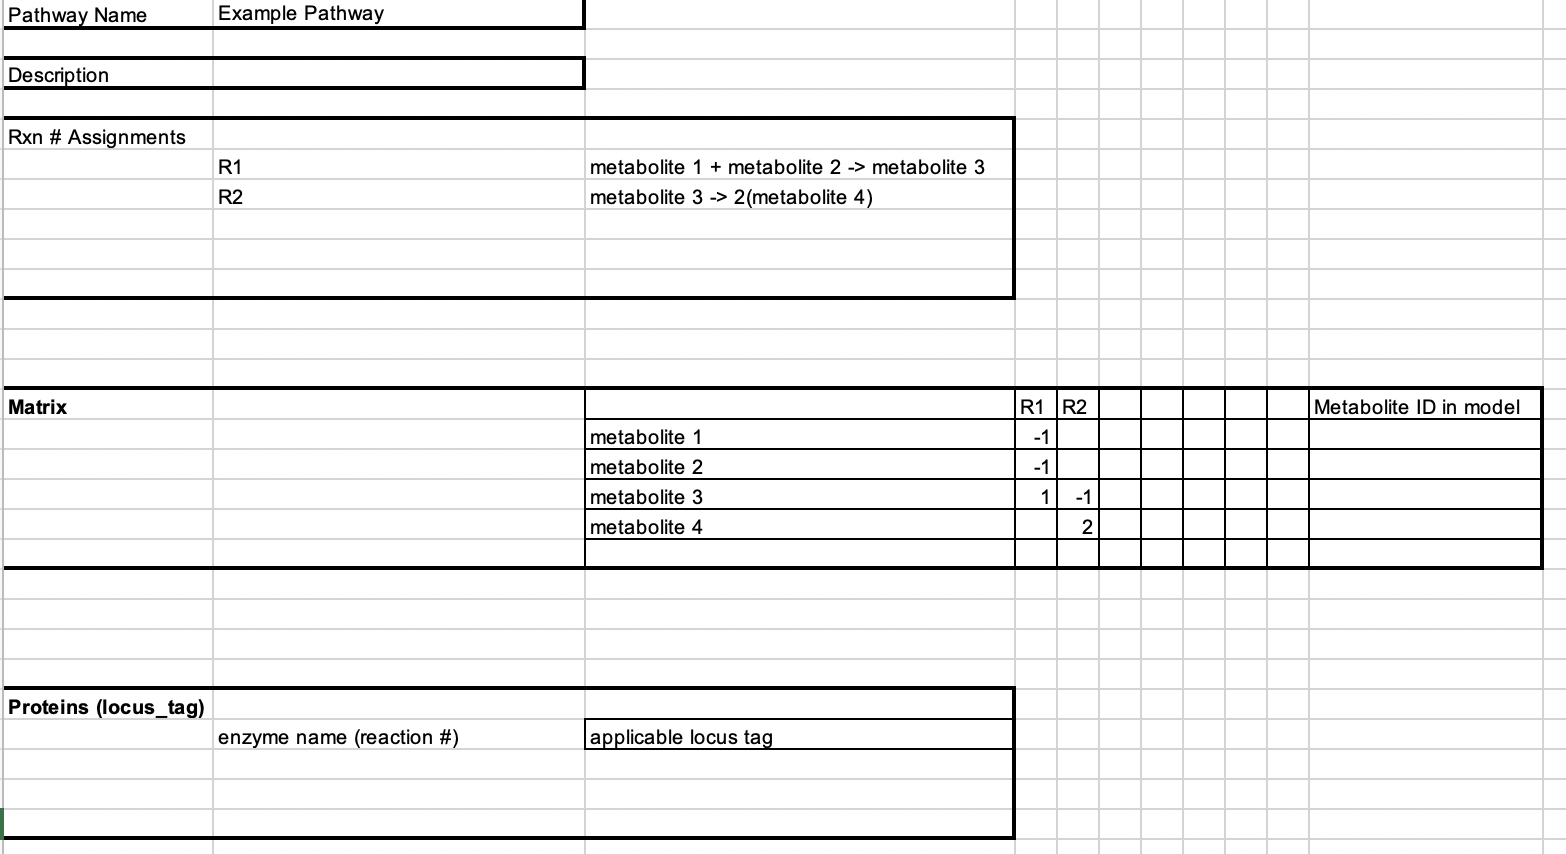
\includegraphics[width=0.7\textwidth]{images/chap8/image01.png}
    \label{fig:ch801}
    \end{figure}
    \FloatBarrier

    \item These can then be added to the model using functions found for matlab \href{https://opencobra.github.io/cobratoolbox/stable/modules/analysis/FBA/index.html}{here} under flux balanced analysis or for python \href{https://cobrapy.readthedocs.io/en/latest/}{here}. 
\end{enumerate}

\subsection{Creating an Objective}
One needs to create an objective for which the model can solve. This is most likely biomass production or a reaction. If it is a reaction, one can just set the model’s objective equal to that reaction. One can also change the objective at any point in a script for analysis.

\subsection{Validating a Model}
Before depending on a model’s results, one should validate the model. First, the model van be validated to not have any inner problems with Cobra using a provided function by Cobra. Ideally, one should also test a situation that is represented in vivo and see if similar optimized results are found. Ideally, with a model being a simplification, validation is an ongoing process. A model will never be perfect and so the more in vivo testing to allow more specified constraints, the stronger a model.

\subsection{Creating Exchanges, Sinks, and Demands}
Boundary reactions fall into the categories of exchange, demand, and sink reactions. They allow the removal or addition of a metabolite into a system. An exchange reaction represents the reversible exchange of an extracellular metabolite, an example being (co2\_e $\Leftrightarrow $) with the $e$ specifying that the metabolite is extracellular. A sink is similar to an exchange reaction in being reversible but involves an intracellular metabolite, an example being (glycogen\_c $\Leftrightarrow $) with the $c$ specifying that the metabolite is a cellular component. Finally, a demand reaction is the irreversible consumption of an intracellular metabolite ($\rightarrow$glucose\_c) These can be added by adding boundaries to the model, specifying the metabolites involved and type of boundary.

\section{Performing the Simulation}
\subsection{Basic Analysis}
FBA can allow multiple forms of analysis. One can first just find the solution of fluxes of each reaction as well as the solved flux of the optimized value. One does this by using a function that optimizes the model according to the objective clarified. One solution provided will be of your objective value, so in the case of an objective being biomass production, the solution for the objective would be the maximum growth rate achieved under the constraints. The other solution will be of all the fluxes of the reactions that allow that maximum growth rate to be achieved. 

\subsection{Flux Variability Analysis}
It is important to note that the model can use a host of solutions, and therefore fluxes, to get the optimized objective value. Therefore, the fluxes of the reactions represent only one possible solution. Therefore, a more robust analysis may be through flux variability analysis. Flux variability analysis finds the minimum and maximum fluxes of the reactions that are allowed to provide a solution that maintains a specified level of the optimized objective value. In other words, I could find the minimum and maximum flux of a certain reaction whose range still allows 50\% of maximum biomass production, or growth rate, to be maintained. 

\subsection{Genetics-based Analysis}
If the model includes gene-reaction assignments, one can also simulate the deletion of specific genes and assess the downstream impact of said deletions on the model.
Another possible method of analysis allows optimization of two different values. For example, let’s say that a team wants to optimize the production of a target metabolite, yet obviously the team also wants the cells to be able to grow effectively. If one were to optimize the model to solve for the highest possible flux of the target molecule production, this found solution may not reflect a solution that is feasible for cellular growth. Media sources can range to support microbes facing deficiencies, therefore simulating growth using growth scripts can become a guessing game. Ideally, one would simultaneously optimize biomass growth as well as the synthesis of our target metabolite. Therefore, we can use OptKnock which allows FBA to solve for the optimal flux distribution that simultaneously optimizes two objective functions, biomass growth as well as the formation of the target metabolite. More information about this approach can be found \href{https://github.com/opencobra/COBRA.tutorials/blob/master/design/optKnock/tutorial_optKnock.m}{here}. Since this is a common approach made by teams using cyanobacteria, a more detailed example is provided below for optimized n-butanol production:
\begin{enumerate} [noitemsep,topsep=0pt]
    \item Constrain the model with biological assumptions
    \begin{enumerate}[noitemsep,topsep=0pt]
        \item Enable secretion routes for the molecules of interest with an upper bound of 1000 (max flux)
        \begin{enumerate}[noitemsep,topsep=0pt]
            \item Exchange={‘EX\_nbut\_e’};
            \begin{enumerate}[noitemsep,topsep=0pt]
                \item \textbf{\textit{Specify the exchange reactions for your metabolites of interest}}
                \end{enumerate}
            \item Bounds=[1000; 1000]
            \item model = changeRxnBounds(model, Exchange, Bounds, ‘u’)
        \end{enumerate}
        \item Set reaction list of reactions to choose to possible delete
        \begin{enumerate}[noitemsep,topsep=0pt]
\item selectedRxnList = \{‘GND’; ‘etc’\}
\begin{enumerate}[noitemsep,topsep=0pt]
    \item \textbf{\textit{Note: I would recommend performing multiple times if you want to speed up analysis (one with the central metabolism fluxes and with another set)}}
    \item \textbf{\textit{These reaction lists must match the reactions listed in the model }}
\end{enumerate}
\end{enumerate}
    \end{enumerate}
\item Generate growth rate and fluxes before optimization
\begin{enumerate}[noitemsep,topsep=0pt]
\item Determine growth rate
\begin{enumerate}[noitemsep,topsep=0pt]
    \item solution = optimizeCbModel(model);
\end{enumerate}
\item Calculate the production of metabolites before running optKnock (before optimization)
\begin{enumerate}[noitemsep,topsep=0pt]
    \item nbutFlux = solution.x(strcmp(model.rxns, ‘EX\_nbut\_e’));
    \item growthRate = solution.f
\end{enumerate}
\end{enumerate}
\item Set up optKnock options
\begin{enumerate}[noitemsep,topsep=0pt]
\item Make the exchange of nbutanol the objective of the outer problem (overproduction)
\begin{enumerate}[noitemsep,topsep=0pt]
    \item options = struct(‘targetRxn’, ‘EX\_nbut\_e’, ‘numDel’, \#);
\begin{enumerate}[noitemsep,topsep=0pt]
    \item The numDel option indicates the optKnock set size upper limit
\end{enumerate}
\end{enumerate}
\item Impose that biomass must be at least 50\% of the biomass of WT
\begin{enumerate}[noitemsep,topsep=0pt]
    \item constrOpt = struct(‘rxnList’, \{\{biomass\}\}, ‘values’, 0.5*solution.f, ‘sense’, ‘G’);
\end{enumerate}
\end{enumerate}
\item Now try to find an optKnock sets (of a max length of 2 as limited earlier)
\begin{enumerate}[noitemsep,topsep=0pt]
    \item optKnockSol = OptKnock, model, selectedRxnList, options, constrOpt);
\end{enumerate}
\item Generate n-butanol flux (production) and growth rate after optimization
\begin{enumerate}[noitemsep,topsep=0pt]
\item nbutFluxO1 = optKnockSol.fluxes(strcmp(model.rxns, ‘EX\_nbut\_e’))
\item growthRateO1 = optKnockSol.fluxes(strcmp(model.rxns, biomass))
\end{enumerate}
\end{enumerate}
\subsection{Data Visualization}
COBRA provides the quantitative data regarding growth rates and fluxes, however a long list of numbers does not lend itself for visualization and first-glance analysis. A metabolic map shows a set of chosen reactions of a model on which flux numbers can be visualized both as their raw numbers and through thickening of arrows to reflect flux levels. One such example is observed from Miami\_OH’s 2021 iGEM team in showing the optimized metabolic flux values for reactions involved in the central metabolism of a model of the cyanobacterium \textit{Synechococcus elongatus} PCC 7942 originally designed by Jared Broddrick in Susan Golden’s lab at University of California-San Diego \parencite{Broddrick2016}. These maps can be accessed through Matlab if properly incorporated into the model itself. However, a more accessible program for visualizing flux data on metabolic maps is \href{https://escher.github.io/}{Escher}. Escher has an online platform that is very intuitive as well as a module for python that provides more robust, although less intuitive, analysis. The original program provides many in-built models and metabolic maps, but available extensions provide additional opportunities to upload personal data. One example is the flux-balance analysis extension which allows flux values to be mapped with different thicknesses indicating different levels of flux. \\ \\
Python, R and matlab also provide graphing capabilities and therefore users can use whichever they feel the most comfortable with. If a user is unfamiliar with coding in general, matlab will probably provide more intuitive graphing capabilities. Conversely, although python tends to have a steeper learning curve, once knowledgeable of modules such as numpy and matplot, python is more immediately easier to use to manipulate data. Therefore, if one is familiar with coding, python and R are suggested as they provide flexibility that only the most advanced matlab users can simulate using matlab.

\begin{figure}[!htbp]
    \centering
    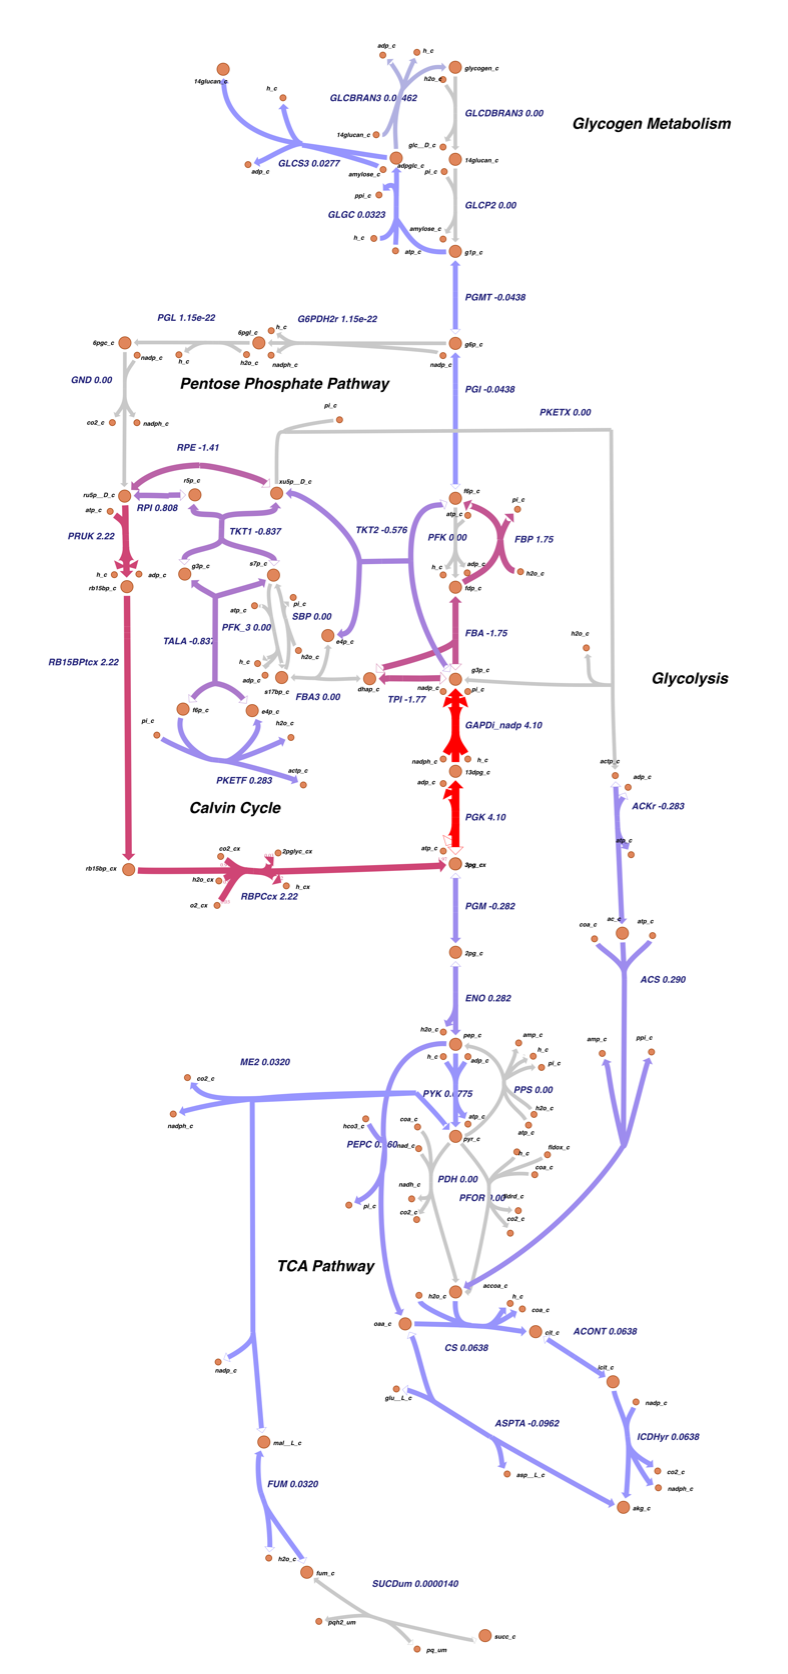
\includegraphics[width=0.6\textwidth]{images/chap8/image02.png}
    \label{fig:ch802}
\end{figure}
\FloatBarrier

\subsection{Integrating Regulation into a Model}
A cell does not just allow its reactions to occur randomly, but instead must maintain strict control over which reactions are active and which are not. Therefore, a cell regulates the expression of the genes whose products involve enzymes or other products that control the activity of these reactions. This regulation can be incorporated into a model based on some mathematical principles, primarily the derived Hill function based on the law of mass action. Since the focus of this handbook is to provide practical assistance over understanding the theory, we direct the reader to other readings for further understanding of this derivation. Ultimately, the expression of a gene is controlled by its promoter which can be bound to by a transcription factor (TF) to either turn the promoter on, thereby expressing the gene, or turn the promoter off, thereby preventing or lowering gene expression. This idea can be represented through the chemical equation $promoter+TF \leftrightarrow promoter.TF$. Therefore, based on the assumption of rapid binding for rapid equilibrium, if a transcriptional factor turns off a gene, it can be represented through the differential equation of
 $$\frac{d[Promoter.TF]}{dt}=kon[promoter][TF]-koff[promoter.TF]=0$$
If a gene is expressed, it is transcribed to become mRNA. Therefore, one can also derive the equation $$\frac{d[mRNA]}{dt}=k1[promoter.TF]$$ The previous two equations can be combined and further derived to become
$$\frac{[Protein]}{dt}=[Protein]=\frac{[TF]}{Kd+[TF]}-d2[Protein]$$ 
Kd is the amount of TF-promoter bindings required to reach half of the max amount of protein that can be produced. Notably, similar to the kinetics based model requiring data regarding enzymatic kinetics, this approach requires knowledge of the binding profile for transcriptional regulators and subsequent mRNA transcript levels \parencite{Vivek-Anath2016}. Notably, this can be found based on omics data which is growing in accessibility due to the development of high-throughput technologies.





% =====================================================================
% ============================== CHAPTER ==============================
% =====================================================================

\chapter{Past Projects}

\epigraph{Unfortunately, no one can be told what the Matrix is. You have to see it for yourself.}{\textit{Morpheus to Lennart, iGEM Bielefeld-CeBiTec 2021}}



\section{Algae}

\textbf{\uppercase{Humboldt\_Berlin}} 
\FloatBarrier
\begin{table}[h]
\begin{tabular}{lllll}
\textbf{Location:} & Germany & \multicolumn{1}{|l}{} & \textbf{Track:}   & Environment \\
\textbf{Region:}   & Europe   & \multicolumn{1}{|l}{} & \textbf{Section:} & Overgraduate \\
\textbf{Year:}     & 2019   & \multicolumn{1}{|l}{} & \textbf{Awards:}  & Gold Medal
\end{tabular}
\end{table} 
\FloatBarrier
\noindent\textbf{Chlamylicious - Establishing Chlamy at iGEM while degrading plastic} \vspace{.2cm}\\ 
Chlamydomonas reinhardtii is a unicellular algae with promising prospects for synthetic biology. Its ability to grow photoautotrophically makes it an ideal chassis to tackle a variety of problems in an environmentally friendly way. Our goal is to adress the worldwide problem of plastic pollution by creating a catalogue of genetic parts for C. reinhardtii that can enable the algae to degrade PET plastic. By combining different functional genetic parts we plan to address the problem from multiple perspectives. To do so, we are designing and building a reproducible low-budget cultivation setup which will aid us and others in the process of collecting data of algal growth under the influence of transgenic constructs and other parameters.latile tool for dealing with a complex problem such as plastic pollution from different perspectives. 
\vspace{2cm} $ $
\pagebreak

\noindent\textbf{\uppercase{Cambridge-JIC}} 
\FloatBarrier
\begin{table}[h]
\begin{tabular}{lllll}
\textbf{Location:} & United Kingdom & \multicolumn{1}{|l}{} & \textbf{Track:}   & Foundational Advance \\
\textbf{Region:}   & Europe   & \multicolumn{1}{|l}{} & \textbf{Section:} & Overgraduate \\
\textbf{Year:}     & 2016   & \multicolumn{1}{|l}{} & \textbf{Awards:}  & Gold Medal
\end{tabular}
\end{table} 
\FloatBarrier
\noindent\textbf{InstaChlam - a toolkit for chloroplast transformation} \vspace{.2cm}\\
As the factory floor of the plant cell, the chloroplast can be engineered to produce many important compounds, such as biofuels and vaccine antigens, with yields approximately 50X greater than the rest of the cell. However, little of this potential has been exploited, in the absence of a time-efficient chloroplast transformation protocol. Using the alga Chlamydomonas reinhardtii as our chassis, our transformation toolbox aims to shift the focus of plant engineering, by reducing the time needed for a homoplasmic chloroplast transformation from months to 1-2 weeks. We have created a library of Chlamydomonas-optimised parts in the Phytobrick standard, with a view to expressing Cas9 in the Chlamydomonas chloroplast for the first time. We hope to use it to propagate genetic modifications among all copies of the chloroplast genome, within a single generation. We will also develop a low-cost, open source Chlamydomonas growth facility and gene gun to complement our protocol. 
\vspace{2cm}

\noindent\textbf{\uppercase{FAFU-CHINA}} 
\FloatBarrier
\begin{table}[h]
\begin{tabular}{lp{2.5cm}llll}
\textbf{Location:} & China & \multicolumn{1}{|l}{} & \textbf{Track:}   & Environment \\
\textbf{Region:}   & Asia   & \multicolumn{1}{|l}{} & \textbf{Section:} & Undergraduate \\
\textbf{Year:}     & 2016   & \multicolumn{1}{|l}{} & \textbf{Awards:}  & Gold Medal
\end{tabular}
\end{table} 
\FloatBarrier
\noindent\textbf{Cry For Mosquito} \vspace{.2cm}\\
In 2016, FAFU-CHINA will attach the effective protoxin gene, which isolated from Bacillus thuringiensis contained the characteristic of high efficient mosquito control, to Chlamydomonas reinhardtii as the chassis organism for cloning. However, there are many problems in the practical application by using Bacillus thuringiensis, such as the bacterial pollution of waters, or the poor timeliness which Bt. strains cannot colonize in the water. Our team use the pertinent literature as the basis for selecting the appropriate biological chassis, combinating the toxic protein, which in order to increase the effect of killing mosquito larvae and reduce the Bt. toxin tolerance. on the basis of Chlamydomonas reinhardtii expression system to optimize gene,enhance expression of results, and reconstruct the engineered bacteria in natural environment, we can settle the problems mentioned above. 
\vspace{2cm} $ $
\pagebreak

\noindent\textbf{\uppercase{SZU-China}} 
\FloatBarrier
\begin{table}[h]
\begin{tabular}{lp{2.5cm}llll}
\textbf{Location:} & China & \multicolumn{1}{|l}{} & \textbf{Track:}   & Energy \\
\textbf{Region:}   & Asia   & \multicolumn{1}{|l}{} & \textbf{Section:} & Undergraduate \\
\textbf{Year:}     & 2016   & \multicolumn{1}{|l}{} & \textbf{Awards:}  & Gold Medal
\end{tabular}
\end{table} 
\FloatBarrier
\noindent\textbf{Light Hygician} \vspace{.2cm}\\
Hydrogen energy, is of great potential in the future with its zero-emission and high-efficiency. However, the fact that few efficient and environment-friendly methods for hydrogen production constrains its application. Therefore, our team develope a biological production way, using the green algae - Chlamydomonas reinhardtii. Since the hydrogenase activity will be inhibited in absence of oxygen and the algae can’t stop photosynthesis forever, we design a switch altering between 2 states in which light wavelength serves as extraneous inducible factor. In specific alternation, we utilize miRNA targeting the expression of key protein in photosynthesis, so we can select the hydrogen-production switch by regulating miRNA. In our design, we utilize Yeast-Two-Hybrid system and light-mediated fusion protein constructing a gene circuit where microRNA can regulate the specific downstream protein expression, and finally keep algae producing H2. In this way, the blue light switch regulate chlamydomonas producing intemittent hydrogen efficienctly, acting as blue-flame bubbling.
\vspace{2cm}

\noindent\textbf{\uppercase{Linkoping\_Sweden}} 
\FloatBarrier
\begin{table}[h]
\begin{tabular}{lp{2.5cm}llll}
\textbf{Location:} & Sweden & \multicolumn{1}{|l}{} & \textbf{Track:}   & Environment \\
\textbf{Region:}   & Europe   & \multicolumn{1}{|l}{} & \textbf{Section:} & Overgraduate \\
\textbf{Year:}     & 2016   & \multicolumn{1}{|l}{} & \textbf{Awards:}  & Gold Medal
\end{tabular}
\end{table} 
\FloatBarrier
\noindent\textbf{A CRSIPR case for biofuel} \vspace{.2cm}\\
This year LiU iGEM will be a part of the search for alternative energy sources, this as a result of global warming due to excessive use of fossil fuels. For this we will use CRISPR/Cas9 in unicellular model algae Chlamydomonas reinhardtii, which has shown great potential for production of biofuels. Previous research has attempted to modify algae to promote the lipid synthesis thereby optimizing them for biofuel production. In this project we want to create new Biobricks consisting of inducible promoters to couple with a CRISPR/Cas9-system in C. reinhardtii. The reason for the inducible promoters is to avoid complications such as toxicity of a constitutively active Cas9. By causing cultures of algae to undergo genetic modification in response to high intensity light we believe we can solve this problem. With this method genes can be targeted in the model algae in order to regulate the lipid synthesis. \\ \\
\vspace{2cm}  $ $
\pagebreak

\noindent\textbf{\uppercase{USP\_UNIFESP-Brazil}} 
\FloatBarrier
\begin{table}[h]
\begin{tabular}{lp{2.5cm}llll}
\textbf{Location:} & Brazil & \multicolumn{1}{|l}{} & \textbf{Track:} & Manufacturing \\
\textbf{Region:} & Latin America   & \multicolumn{1}{|l}{} & \textbf{Section:} & Overgraduate \\
\textbf{Year:}     & 2016   & \multicolumn{1}{|l}{} & \textbf{Awards:}  & Gold Medal
\end{tabular}
\end{table} 
\FloatBarrier
\noindent\textbf{AlgAranha} \vspace{.2cm}\\
The objective of this project is to produce a biomaterial for immobilizing proteins initially directed to application on burns, using immobilized enzibiotics. The term "enzibiotics" refers to the junction of the words "enzyme" and "antibiotic," this is enzymes exhibiting antimicrobian activity. For immobilizing these biomolecules will be used gene recombination techniques, adding the polymerization domains in the enzibiotic molecule, compatible with the spider silk proteins. Both will be produced in recombinant microalgae by nuclear transformation of model microorganism Chlamydomonas reinhardtii. The project will be executed by group of undergraduates and graduate students in the context of iGEM. It is expected to achieve spider silk fiber production and its initial characterization for antimicrobial activity and mechanical properties, as well as the productivity evaluation in the proposed system. From these results, we can evaluate the application of this immobilizer in other biotechnological applications such as biotransformation, biosensors, biomaterials and textile industry.
\vspace{2cm}

\textbf{\uppercase{UConn}}
\FloatBarrier
\begin{table}[h]
\begin{tabular}{lp{2.5cm}llll}
\textbf{Location:} & United States & \multicolumn{1}{|l}{} & \textbf{Track:}   & Energy \\
\textbf{Region:}   & North America   & \multicolumn{1}{|l}{} & \textbf{Section:} &  \\
\textbf{Year:}     & 2017   & \multicolumn{1}{|l}{} & \textbf{Awards:}  &
\end{tabular}
\end{table}
\FloatBarrier
\noindent	extbf{} \vspace{.2cm}\\
An Algaeneious Approach to Continuous Cultures for Biofuel Production
Biofuels are a promising, nearly carbon-neutral alternative fuel source, often derived from algal lipid production. Previous methods of fuel harvest have relied on destructive means of extraction, but we aim to upregulate the excretion of lipids, allowing for potential harvest by physical separation. Our goal is to enhance the algal lipid production and extracellular transport in Nannochloropsis oceanica, a well characterized species with high lipid content. This will be achieved by upregulating the endogenous lipid production enzymes of the cell with high expression promoters and transfecting algae with an ATP binding cassette transporter from Arabdopsis thaliana. Next steps will include developing a system to physically separate excreted lipid from the algal biomass, while maintaining a productive continuous culture.

% ========== TEMPLATE ==========
\iffalse
\textbf{\uppercase{Team\_Name}} 
\FloatBarrier
\begin{table}[h]
\begin{tabular}{lp{2.5cm}llll}
\textbf{Location:} & Germany & \multicolumn{1}{|l}{} & \textbf{Track:}   & Environment \\
\textbf{Region:}   & Europe   & \multicolumn{1}{|l}{} & \textbf{Section:} & Undergraduate \\
\textbf{Year:}     & 2019   & \multicolumn{1}{|l}{} & \textbf{Awards:}  & Gold Medal
\end{tabular}
\end{table} 
\FloatBarrier
\noindent\textbf{TITLE} \vspace{.2cm}\\
Abstract
\fi

\pagebreak
\section{Cyanobacteria}

\textbf{\uppercase{Amsterdam}} \FloatBarrier \begin{table}[h] \begin{tabular}{lp{2.5cm}llll} \textbf{Location:} & Netherlands & \multicolumn{1}{|l}{} & \textbf{Track:}   & Energy \\ \textbf{Region:}   & Europe   & \multicolumn{1}{|l}{} & \textbf{Section:} &  \\ \textbf{Year:}     & 2015   & \multicolumn{1}{|l}{} & \textbf{Awards:}  & \end{tabular} \end{table} \FloatBarrier \noindent\textbf{Synthetic Romance - Harnessing the power of Cyanobacteria to construct a sustainable consortia} \vspace{.2cm}\\  Researchers are starting to recognize that synthetic ecosystems consortia of multiple bacterial species can be used for higher yields robustness and more diverse purposes. Our goal is to tap into this potential by creating a self-sustaining bio-factory of cyanobacteria - little fellows that need only CO2 and light - and product-producing E. coli the general workhorse of the synthetic biology world. The cyanobacteria will create sugars from CO2 and sunlight which it will release and feed to E. coli as a result of our applied synthetic genetic circuits. E. coli will then be engineered to use these sugars to create a product. In our proof-of-concept bio-factory this product will be fuel. This platform however can be expanded to produce any product E. coli can make - medicine plastics commodity chemicals - as long as it is fueled by the cyanobacteria that only needs light and CO2.
\vspace{2cm}

\textbf{\uppercase{LaVerne-Leos}} \FloatBarrier \begin{table}[h] \begin{tabular}{lp{2.5cm}llll} \textbf{Location:} & United States & \multicolumn{1}{|l}{} & \textbf{Track:}   & Energy \\ \textbf{Region:}   & North America   & \multicolumn{1}{|l}{} & \textbf{Section:} &  \\ \textbf{Year:}     & 2015   & \multicolumn{1}{|l}{} & \textbf{Awards:}  & \end{tabular} \end{table} \FloatBarrier \noindent\textbf{Using Zeaxanthin and Tocopherol to protect cyanobacteria from the toxic effects of free fatty acids} \vspace{.2cm}\\ Free fatty acids are biofuel precursors.  We focused on using zeaxanthin to counter the toxic effects of increased free fatty acids in an altered Synechococcus elongatus 7942 strain. Zeaxanthin acts as an antioxidant stabilizes the membrane and is needed for electron transport chain function. To increase the concentration of zeaxanthin and its precursors we introduced a circuit containing parts of the zeaxanthin synthesis pathway. The La Cañada subset of our team focused on tocopherol a metabolite that has similar properties to zeaxanthin in cyanobacteria. Tocopherol acts as an antioxidant protects the cell from lipid peroxidation and enhances photosynthesis. A circuit was made with the gene p-hydroxyphenylpyruvate dioxygenase to catalyze the formation of homogenistic acid the rate limiting step of tocopherol synthesis. In an attempt to further increase the production of fatty acids both zeaxanthin and tocopherol circuits are dynamically regulated utilizing a fatty acid-sensitive promoter-repressor system pLR and FadR.
\vspace{2cm} $ $
\pagebreak

\textbf{\uppercase{Reading}} \FloatBarrier \begin{table}[h] \begin{tabular}{lp{2.5cm}llll} \textbf{Location:} & United Kingdom & \multicolumn{1}{|l}{} & \textbf{Track:}   & Energy \\ \textbf{Region:}   & Europe   & \multicolumn{1}{|l}{} & \textbf{Section:} &  \\ \textbf{Year:}     & 2015   & \multicolumn{1}{|l}{} & \textbf{Awards:}  & \end{tabular} \end{table} \FloatBarrier \noindent\textbf{Innovating living photovoltaics: Renewable energy from Cyanobacteria} \vspace{.2cm}\\
Conventional photovoltaics provide a clean source of renewable energy but have the disadvantages of being expensive and containing toxic materials. This years iGEM project was to develop a cheaper non-toxic alternative to conventional fuel cells; using synthetic biology. Biological photovoltaics (BPV) are a promising candidate to provide an alternative. Our BPV uses the Cyanobacterium Synechocystis sp. PCC 6803 as the electron source. Using a purpose built fuel cell and Synechocystis which has been genetically modified to improve interactions between the bacterium and the anode surface enables the BPV to generate a greater voltage. This BPV will be considered for large scale usage in homes and communities worldwide as a cheap simple and clean alternative to conventional energy sources. 
\vspace{2cm}

\textbf{\uppercase{Uniandes\_Colombia}} \FloatBarrier \begin{table}[h] \begin{tabular}{lp{2.5cm}llll} \textbf{Location:} & Colombia & \multicolumn{1}{|l}{} & \textbf{Track:}   & Information Processing \\ \textbf{Region:}   & Latin America   & \multicolumn{1}{|l}{} & \textbf{Section:} &  \\ \textbf{Year:}     & 2015   & \multicolumn{1}{|l}{} & \textbf{Awards:}  & \end{tabular} \end{table} \FloatBarrier \noindent\textbf{Building a Bio-Electronic Clock} \vspace{.2cm}\\ 
We are currently working on a bio-digital clock as a proof-of-concept project dealing with the integration of biological and electronic circuits. We plan to modify the circadian clock Kai protein system of cyanobacteria Synechococcus elongatus by hooking it to the AHL-producing half of the Lux quorum sensing system of Vibrio fischerii. The sensing portion of the Lux system will reside in modified Shewanella oneidensis engineered to produce changes in its electrical resistance in response to changing levels of AHL using this speciess control of cytochrome production. Finally another key component of our project is the design and construction of the eletcronic hardware necessary to measure S. oneidensiss changes in electrical conductance and act as an interface between this biological circuit and any electronic circuit it is to be coupled with in this example a digital clock.
\vspace{2cm} $ $
\pagebreak

\textbf{\uppercase{Yale}} \FloatBarrier \begin{table}[h] \begin{tabular}{lp{2.5cm}llll} \textbf{Location:} & United States & \multicolumn{1}{|l}{} & \textbf{Track:}   & Foundational Advance \\ \textbf{Region:}   & North America   & \multicolumn{1}{|l}{} & \textbf{Section:} &  \\ \textbf{Year:}     & 2015   & \multicolumn{1}{|l}{} & \textbf{Awards:}  & \end{tabular} \end{table} \FloatBarrier \noindent\textbf{Developing a Framework for the Genetic Manipulation of Non-Model and Environmentally Significant Microbes} \vspace{.2cm}\\ 
We established a framework for implementing genetic manipulation techniques—specifically multiplex automated genome engineering (MAGE) and CRISPR-Cas9 systems—into non-model environmentally significant microbes using standard biological parts. The framework involves two components: (1) propagation and selection of cultures and (2) manipulation of cell genomes by MAGE and/or CRISPR. We identified design considerations for both components of the framework and experimentally validated propagation and selection considerations using cyanobacterial strain Synechococcus sp. PCC 7002 (a fast-growing cyanobacterium capable of lipid biofuel production) and Sinorhizobium tropici CIAT (a nitrogen-fixing rhizobium which forms root nodules in legume plants). We then developed a workflow for the design construction and testing of MAGE and CRISPR technologies in non-model prokaryotes. The insights we gained from validating the propagation component of our workflow will serve to improve the versatility and robustness of our framework and will inform the development of tools for genetic manipulation in other non-model organisms.
\vspace{2cm}

\textbf{\uppercase{Chalmers\_Gothenburg}} \FloatBarrier \begin{table}[h] \begin{tabular}{lp{2.5cm}llll} \textbf{Location:} & Sweden & \multicolumn{1}{|l}{} & \textbf{Track:}   & Environment \\ \textbf{Region:}   & Europe   & \multicolumn{1}{|l}{} & \textbf{Section:} &  \\ \textbf{Year:}     & 2016   & \multicolumn{1}{|l}{} & \textbf{Awards:}  & \end{tabular} \end{table} \FloatBarrier \noindent\textbf{Turning pollution into a solution} \vspace{.2cm}\\ 
Current methods of chemical synthesis from petroleum have led to great environmental disruption and continue to be a strong contributor to the emission of carbon dioxide. To overcome this problem biosynthesis is the most viable alternative. The main drawback of biosynthesis is the high price of raw material comprising over 60\% of the production cost. Our solution for this complex problem is to create a self-sustaining co-culture of microorganisms that produces its own raw material using light and carbon dioxide. Cyanobacteria provide the carbon source for the production organism which in exchange produces an essential amino acid for the cyanobacteria while creating the desired product. By making several species compatible with this synthetic symbiosis the platform will allow efficient conversion of atmospheric carbon dioxide into products in an environmentally friendly and sustainable way.
\vspace{2cm} $ $
\pagebreak

\textbf{\uppercase{CSU\_Fort\_Collins}} \FloatBarrier \begin{table}[h] \begin{tabular}{lp{2.5cm}llll} \textbf{Location:} & United States & \multicolumn{1}{|l}{} & \textbf{Track:}   & New Application \\ \textbf{Region:}   & North America   & \multicolumn{1}{|l}{} & \textbf{Section:} &  \\ \textbf{Year:}     & 2016   & \multicolumn{1}{|l}{} & \textbf{Awards:}  & \end{tabular} \end{table} \FloatBarrier \noindent\textbf{CyanoLogic: A novel modular production system in Synechocystis 6803} \vspace{.2cm}\\ 
Lights Quorum Action! Boolean logic is used in computer processes by stipulating necessary inputs to produce a desired outcome. We designed a logic gate in Synechocystis sp. PCC 6803 to optimize product production. Utilizing the Boolean operator AND gene expression accommodates the organism’s natural metabolic regulation combined with the quorum sensing mechanism from Vibrio fischeri to create an autoinduction system. With the cost of large scale production in mind our system eliminates the need for expensive induction molecules such as IPTG. Under the control of light and a quorum of cells the T7 promoter from T7 bacteriophage drives production of a wide range of products from biofuels to pharmaceuticals. CyanoLogic coming soon to a lab near you!
\vspace{2cm}

\textbf{\uppercase{Edinburgh\_OG}} \FloatBarrier \begin{table}[h] \begin{tabular}{lp{2.5cm}llll} \textbf{Location:} & United Kingdom & \multicolumn{1}{|l}{} & \textbf{Track:}   & New Application \\ \textbf{Region:}   & Europe   & \multicolumn{1}{|l}{} & \textbf{Section:} &  \\ \textbf{Year:}     & 2016   & \multicolumn{1}{|l}{} & \textbf{Awards:}  & \end{tabular} \end{table} \FloatBarrier \noindent\textbf{ExpandED: Tools For Rapid Prototyping in Non-Model Hosts} \vspace{.2cm}\\ 
Industrial biotechnology is greatly dependent on the use of model organisms such as Escherichia coli and Saccharomyces cerevisiae. The minimal cell is a future ambition of synthetic biology however there remains a vast untapped reservoir of non-model organisms each with diverse and unique traits for exploitation. It is a lack of tools designed for native producer organisms that often limits use as effective bio-factories. Today advance genetic engineering techniques such as CRISPR/Cas editing and MoClo assembly methods allow rapid strain prototyping at unprecedented ease and cost. Our team aim to demonstrate the potential speed and power of these techniques in developing three diverse platform strains and respective parts libraries for use by research groups iGEM teams commercial organisations and citizen scientists.
\vspace{2cm} $ $
\pagebreak

\textbf{\uppercase{IngenuityLab\_Canada}} \FloatBarrier \begin{table}[h] \begin{tabular}{lp{2.5cm}llll} \textbf{Location:} & Canada & \multicolumn{1}{|l}{} & \textbf{Track:}   & New Application \\ \textbf{Region:}   & North America   & \multicolumn{1}{|l}{} & \textbf{Section:} &  \\ \textbf{Year:}     & 2016   & \multicolumn{1}{|l}{} & \textbf{Awards:}  & \end{tabular} \end{table} \FloatBarrier \noindent\textbf{DNA assisted assembly of modular nanowires} \vspace{.2cm}\\ 
Our project seeks to manufacture nanostructures. By bridging the two opposite approaches together we have devised a method to create a modular nanowires. With DNA Origami self assembling properties organize the DNA strand into patterns by using the local forces to find the lowest energy configuration which is an Bottom-Up approach. To fold the DNA strand into a well defined structure using DNA staples is an example of Top-Down approach. DNA has many advantages over traditional materials such as biological compatibility low manufacturing cost and the information regarding shape and size is carried over upon replication. Individual modules are 30-40 nm long 3D Structures with hollow cavity that acts as scaffold for the Gold nanowires. They self assemble into long nanowires and we attached photosystem II protein from the Synechocystis 6803 at one end of the wire to create a high efficiency machinery to harvest solar energy.
\vspace{2cm}

\textbf{\uppercase{Marburg}} \FloatBarrier \begin{table}[h] \begin{tabular}{lp{2.5cm}llll} \textbf{Location:} & Germany & \multicolumn{1}{|l}{} & \textbf{Track:}   & New Application \\ \textbf{Region:}   & Europe   & \multicolumn{1}{|l}{} & \textbf{Section:} &  \\ \textbf{Year:}     & 2016   & \multicolumn{1}{|l}{} & \textbf{Awards:}  & \end{tabular} \end{table} \FloatBarrier \noindent\textbf{SYNDUSTRY - fuse. produce. use.} \vspace{.2cm}\\ 
Globalization radically changed the world we live in; the way we communicate and travel has become much easier. On the downside our need for resources has dramatically increased causing ecological and social problems like land-grabbing and fracking. The emergence of Synthetic Biology is initiating another bio-based industrial revolution. It is time to take the next step towards a sustainable bio-industry. In Syndustry we follow nature’s own design principles by combining the strengths of individual microorganisms for the production of valuable biochemicals. We introduce a novel ‘plug-and-play’ production platform based on artificial endosymbiosis. This system goes beyond co-culturing microbes and overcomes current production limitations in fermentation. By employing cyanobacteria capable of photosynthetic growth we achieve a self-sustainable and versatile production platform for biochemicals from carbon dioxide. Syndustry – fuse. produce. use. is the next industrial revolution and will change the face of the world as we know it today!
\vspace{2cm} $ $
\pagebreak

\textbf{\uppercase{MSU-Michigan}} \FloatBarrier \begin{table}[h] \begin{tabular}{lp{2.5cm}llll} \textbf{Location:} & United States & \multicolumn{1}{|l}{} & \textbf{Track:}   & Manufacturing \\ \textbf{Region:}   & North America   & \multicolumn{1}{|l}{} & \textbf{Section:} &  \\ \textbf{Year:}     & 2016   & \multicolumn{1}{|l}{} & \textbf{Awards:}  & \end{tabular} \end{table} \FloatBarrier \noindent\textbf{Engineering Cyanobacteria for Improved Tolerance to a Freeze/Thaw Cycle} \vspace{.2cm}\\ 
Currently the biotechnologically relevant model strain of cyanobacteria Synechococcus elongatus PCC 7942 lacks resilience to cold temperature perturbations. If large-scale operations for photosynthetic production of industrial compounds are to be realized robustness to unpredictable weather conditions must be considered. Two complementary approaches are being proposed to increase cold adaptation and resistance to freezing in S. elongatus. Previously it was shown the expression of lipid desaturase desA increases the cold-growth tolerance of S. elongatus. We now aim to improve this range by fine-tuning the expression of a riboswitch-controlled desA. We also hypothesize that introduction of SFR2 from Arabidopsis thaliana—responsible for remodeling the outer chloroplast membrane for increased freezing tolerance—will increase cellular viability to freezing events. Through this two-pronged approach we aspire to engineer a cyanobacterial strain that ultimately could be used for the production of industrially-relevant products in unreliable environment conditions.
\vspace{2cm}

\textbf{\uppercase{ULV-LC-CV}} \FloatBarrier \begin{table}[h] \begin{tabular}{lp{2.5cm}llll} \textbf{Location:} & United States & \multicolumn{1}{|l}{} & \textbf{Track:}   & Energy \\ \textbf{Region:}   & North America   & \multicolumn{1}{|l}{} & \textbf{Section:} &  \\ \textbf{Year:}     & 2016   & \multicolumn{1}{|l}{} & \textbf{Awards:}  & \end{tabular} \end{table} \FloatBarrier \noindent\textbf{In vivo production of fatty acid methyl esters in cyanobacteria utilizing the insect methyltransferase DmJHAMT } \vspace{.2cm}\\ 
Biodiesel is mainly composed of fatty acid methyl esters (FAMEs) and is a renewable energy source. Currently FAMEs are synthesized through transesterification of free fatty acids (FFAs) using a methyl donor such as methanol along with an alkaline catalyst to speed up the reaction. Both the extraction of FFAs and the chemicals used in this process are expensive. We intend to reduce the production cost of biodiesel by producing FAMEs in vivo using an insect methyltransferase called Drosophila melanogaster Juvenile hormone acid O-methyltransferase (DmJHAMT) within Synechococcus elongatus PCC 7942. DmJHAMT transfers the methyl groups from endogenous S-adenosyl-L-methionine (SAM) to FFAs therefore synthesizing FAMEs.  To minimize extraction costs we aim to induce self-lysis in Synechococcus at maximum optical densities using quorum sensing.  By regulating the production of autoinducers with promoters of various strengths we plan to tune the optical density at which gene expression is activated.
\vspace{2cm} $ $
\pagebreak

\textbf{\uppercase{UNIK\_Copenhagen}} \FloatBarrier \begin{table}[h] \begin{tabular}{lp{2.5cm}llll} \textbf{Location:} & Denmark & \multicolumn{1}{|l}{} & \textbf{Track:}   & New Application \\ \textbf{Region:}   & Europe   & \multicolumn{1}{|l}{} & \textbf{Section:} &  \\ \textbf{Year:}     & 2016   & \multicolumn{1}{|l}{} & \textbf{Awards:}  & \end{tabular} \end{table} \FloatBarrier \noindent\textbf{CosmoCrops: A modular platform for sustainable bioproduction in space} \vspace{.2cm}\\ 
Space missions face the problems that transporting mass is expensive and the needs of long expeditions are unknown in advance.  It would be revolutionary to have the capacity to manufacture various resources needed without prior knowledge of exact mission requirements.  We have designed a modular co-culture system to accomplish this: containing the cyanobacterium Synechococcus elongatus to use CO2 and light which are plentiful on Mars to produce sucrose.  This is used as a common feedstock by Bacillus subtilis to generate essential end-products.  We used polylactic acid as a proof-of-concept since 3D printers can use it for tools and machine parts.  To examine the co-culture’s practicality in extraterrestrial environments the cutting-edge Jens Martin Mars Chamber was used to test stresses including UV exposure and pressure extremes. We propose that Bacillus’s sporulation ability will enable missions to maintain libraries of strains for constructing a versatile array of materials for future space exploration. 
\vspace{2cm}

\textbf{\uppercase{WashU\_StLouis}} \FloatBarrier \begin{table}[h] \begin{tabular}{lp{2.5cm}llll} \textbf{Location:} & United States & \multicolumn{1}{|l}{} & \textbf{Track:}   & Environment \\ \textbf{Region:}   & North America   & \multicolumn{1}{|l}{} & \textbf{Section:} &  \\ \textbf{Year:}     & 2016   & \multicolumn{1}{|l}{} & \textbf{Awards:}  & \end{tabular} \end{table} \FloatBarrier \noindent\textbf{Super Cells: Overproducing ATP and Electron Donors in E. coli} \vspace{.2cm}\\
The Nitrogen Project of which this iGEM team is a part seeks to drastically reduce the quantity of nitrogen-based fertilizers used in agriculture. Soluble nitrates can “runoff” into water systems with environmental consequences such as algal blooms and human illnesses like methemoglobinemia. If nitrogenase the enzyme in soil bacteria that “fixes” nitrogen gas into usable nitrates can be inserted into plants it would eliminate the need for artificial fertilization. Before this can be done nitrogenase must first be expressed non-diazotrophic bacteria like E. coli. For proper expression however E. coli must have an excess of intracellular ATP and reduced electron donors. We worked to overexpress glycolytic kinases to increase ATP production and overexpress native and foreign electron donors to produce more reduced electron donors. Besides nitrogenase however the intracellular environment of our “super cells” may help produce other recombinant proteins.
\vspace{2cm} $ $
\pagebreak

\textbf{\uppercase{Amsterdam}} \FloatBarrier \begin{table}[h] \begin{tabular}{lp{2.5cm}llll} \textbf{Location:} & Netherlands & \multicolumn{1}{|l}{} & \textbf{Track:}   & Manufacturing \\ \textbf{Region:}   & Europe   & \multicolumn{1}{|l}{} & \textbf{Section:} &  \\ \textbf{Year:}     & 2017   & \multicolumn{1}{|l}{} & \textbf{Awards:}  & \end{tabular} \end{table} \FloatBarrier \noindent\textbf{Photosynthetic magic: Producing fumarate out of thin air using cyanobacterial cell factories} \vspace{.2cm}\\ 
Irrespective of where you come from we all share the global responsibility of ensuring that our societies are sustainable. We have been depleting the world’s resources and filling the atmosphere with abnormal levels of CO2 for too long. Our team has decided to take on this challenge by creating photosynthetic cell factories to directly use the pollutant CO2 as a resource for synthesizing fumarate - a versatile chemical traditionally manufactured from petroleum. We aim to stably produce sense and export fumarate under conditions mimicking industrial settings. Stable production is achieved by activating and evolving different metabolic modules in response to natural day/night cycles. To detect fumarate we developed a biosensor suitable for high-throughput screening. Finally to allow optimal fumarate export we investigate its transport mechanism. These efforts attracted attention from beyond academia as our cell factories may help in taking CO2 out of thin air and into a bio-based economy.
\vspace{2cm}

\textbf{\uppercase{NYMU-Taipei}} \FloatBarrier \begin{table}[h] \begin{tabular}{lp{2.5cm}llll} \textbf{Location:} & Taiwan & \multicolumn{1}{|l}{} & \textbf{Track:}   & Energy \\ \textbf{Region:}   & Asia   & \multicolumn{1}{|l}{} & \textbf{Section:} &  \\ \textbf{Year:}     & 2017   & \multicolumn{1}{|l}{} & \textbf{Awards:}  & \end{tabular} \end{table} \FloatBarrier \noindent\textbf{ Smart AlgaEnergy} \vspace{.2cm}\\
Facing the threatening energy crisis scientists are craving for alternative energy sources. Taking both clean energy productivity and other factors under consideration we have decided to target our project on increasing the oil accumulation in microalgae by multiple approaches. On the one hand we have determined to make microalgae undergo nitrogen starvation to increase its oil accumulation by creating a co-culturing system of microalgae and NrtA-transformed Escherichia coli that can deprive microalgae of nitrogen source. On the other hand we have changed the color of microalgae by transforming pigmentation functions from other species into microalgae cells to enhance its efficiency of photosynthesis. By combining these two approaches we can develop a new intelligent system which can enhance bio-energy production and contribute to the needs of renewable clean energy.
\vspace{2cm} $ $
\pagebreak

\textbf{\uppercase{UCSC}} \FloatBarrier \begin{table}[h] \begin{tabular}{lp{2.5cm}llll} \textbf{Location:} & United States & \multicolumn{1}{|l}{} & \textbf{Track:}   & Manufacturing \\ \textbf{Region:}   & North America   & \multicolumn{1}{|l}{} & \textbf{Section:} &  \\ \textbf{Year:}     & 2017   & \multicolumn{1}{|l}{} & \textbf{Awards:}  & \end{tabular} \end{table} \FloatBarrier \noindent\textbf{Bugs Without Borders} \vspace{.2cm}\\ 
Much of the world struggles with inadequate access to essential medicines and nutrition due to high pharmaceutical prices and unreliable distribution. Our solution is to decentralize production of these resources by engineering the robust cyanobacterium Arthrospira platensis to produce essential medicines and supplements self-sustainably photosynthetically and on-site at healthcare facilities. However due to insufficient research into the genetics of A. platensis we have undertaken two separate engineering endeavors in the metabolically similar Synechococcus elongatus PCC 7942 to produce acetaminophen and human-usable vitamin B12. The genes for acetaminophen production 4ABH and nhoA and those for B12 production ssuE and bluB have been transformed into PCC 7942 with the aim of method validation and subsequent migration to A. platensis once a genetic system has been established.  In addition we are performing a whole genome sequencing of A. platensis UTEX 2340 to further this research and its potential medical applications.
\vspace{2cm}

\textbf{\uppercase{UC\_San\_Diego}} \FloatBarrier \begin{table}[h] \begin{tabular}{lp{2.5cm}llll} \textbf{Location:} & United States & \multicolumn{1}{|l}{} & \textbf{Track:}   & New Application \\ \textbf{Region:}   & North America   & \multicolumn{1}{|l}{} & \textbf{Section:} &  \\ \textbf{Year:}     & 2017   & \multicolumn{1}{|l}{} & \textbf{Awards:}  & \end{tabular} \end{table} \FloatBarrier \noindent\textbf{SynEco: A Xenobiotics-derived Co-culture System of S. elongatus and E. coli for Applications in Bioproduction} \vspace{.2cm}\\ 
Currently the biofuel industry uses glucose as feedstock for E. coli. Methods to prevent contamination require expensive process sterilization or excess antibiotics dosage which become ineffective over time by promoting antibiotic resistance. In our project we use a xenobiotic approach to engineer autotrophic cyanobacteria Synechococcus elongatus PCC 7942 to produce the rare sugar D-tagatose in a five-step enzymatic pathway. After detecting tagatose via HPLC we will seek to engineer a transporter for tagatose secretion a mechanism that is currently not known. The cyanobacteria will be harnessed in conjunction with genetically engineered E. coli that can metabolize tagatose; by using a multifaceted approach we could leverage xenobiotic technology in a unique way to create a novel production platform that uses tagatose as a nutrient source and an anti-contamination agent. Because our system utilizes photosynthetic cyanobacteria to cheaply produce the rare sugar carbon source our co-culture system is both self-sustainable and cost-effective.
\vspace{2cm} $ $
\pagebreak

\textbf{\uppercase{WashU\_StLouis}} \FloatBarrier \begin{table}[h] \begin{tabular}{lp{2.5cm}llll} \textbf{Location:} & United States & \multicolumn{1}{|l}{} & \textbf{Track:}   & Environment \\ \textbf{Region:}   & North America   & \multicolumn{1}{|l}{} & \textbf{Section:} &  \\ \textbf{Year:}     & 2017   & \multicolumn{1}{|l}{} & \textbf{Awards:}  & \end{tabular} \end{table} \FloatBarrier \noindent\textbf{Operation: Ultraviolet} \vspace{.2cm}\\ 
Due to numerous climate effects photosynthetic organisms are being damaged due to increased levels of harmful UV-B radiation. Luckily many organisms exist that have a natural resistance to this kind of radiation. Using genes from the tardigrade species Ramazzottius Varieornatus the bacteria species Deinococcus Radiodurans and a strain of cyanobacteria we hope to induce resistance to UV-B radiation damage. In order to demonstrate proof of these genes’ utility our first step was to transform the genes into E. Coli. From there we planned to test these transformed cells in our Environmental Simulation System by irradiating the cells and comparing their growth to that of a control. So far we have found that E. Coli cells with Dsup are substantially more resistant to UV-B radiation and we have also recorded preliminary data on uvsE as well. Currently we are transforming the four genes into cyanobacteria and testing them under UV-B light.
\vspace{2cm}

\textbf{\uppercase{Worldshaper-Nanjing}} \FloatBarrier \begin{table}[h] \begin{tabular}{lp{2.5cm}llll} \textbf{Location:} & China & \multicolumn{1}{|l}{} & \textbf{Track:}   & High School \\ \textbf{Region:}   & Asia   & \multicolumn{1}{|l}{} & \textbf{Section:} &  \\ \textbf{Year:}     & 2017   & \multicolumn{1}{|l}{} & \textbf{Awards:}  & \end{tabular} \end{table} \FloatBarrier \noindent\textbf{Self-sinking Algae for CO2 Sequestration} \vspace{.2cm}\\ 
Increasing level of carbon dioxide in earths atmosphere is the main reason of global warming. Thus it has become important to slow down the accumulation rate or reduce the amount of carbon dioxide in atmosphere. Here we hope to develop an efficient biological carbon dioxide sequestration system using Synchronous sp. PCC 7002. The capability of CO2 capturing and storage of the algae was improved by inserting foreign genes encoding rubisco and starch synthase. The modified strain was also designed to have an expression of a metal binding protein on its pilus to increase weight and deactivate pilus slowly which would finally cause the alga to sink to the sea bottom permanently so as to cut off the carbon from being reused.
\vspace{2cm} $ $
\pagebreak

\textbf{\uppercase{Duesseldorf}} \FloatBarrier \begin{table}[h] \begin{tabular}{lp{2.5cm}llll} \textbf{Location:} & Germany & \multicolumn{1}{|l}{} & \textbf{Track:}   & Foundational Advance \\ \textbf{Region:}   & Europe   & \multicolumn{1}{|l}{} & \textbf{Section:} &  \\ \textbf{Year:}     & 2018   & \multicolumn{1}{|l}{} & \textbf{Awards:}  & \end{tabular} \end{table} \FloatBarrier \noindent\textbf{Trinity - towards an engineered co-culture toolbox} \vspace{.2cm}\\ 
Co-cultures are found in all conceivable entities such as the human gut cheese or plants but good tools to study those communities are currently not given. Indeed we created a modularly built toolbox using not only three different dependencies but also three different organisms: With Escherichia coli Saccharomyces cerevisiae and Synechococcus elongatus our team engineered a system based on nutrient exchange. Here phosphate is provided through oxidation of phosphite nitrogen source produced by melamine breakdown whilst carbon source is provided by Synechococcus elongatus. Two additional independent approaches are designed too. The first includes regulation via cross-feeding by amino acid auxotrophies and production: lysine by Escherichia coli and leucine by Saccharomyces cerevisiae. The other utilizes regulated self-lysis via quorum sensing molecules to control cell density by a phage lysis gene. This engineered toolbox opens a wide range of possibilities to create microbial communities for different purposes such as synthetic probiotics.
\vspace{2cm}

\textbf{\uppercase{NU\_Kazakhstan}} \FloatBarrier \begin{table}[h] \begin{tabular}{lp{2.5cm}llll} \textbf{Location:} & Kazakhstan & \multicolumn{1}{|l}{} & \textbf{Track:}   & Environment \\ \textbf{Region:}   & Asia   & \multicolumn{1}{|l}{} & \textbf{Section:} &  \\ \textbf{Year:}     & 2018   & \multicolumn{1}{|l}{} & \textbf{Awards:}  & \end{tabular} \end{table} \FloatBarrier \noindent\textbf{From a Dangerous Waste to Functional Nanomaterials: Bioremediation of Sour Crude Oil Waste using Cyanobacteria} \vspace{.2cm}\\ 
Accumulation of a hydrogen sulfide as a consequence of sulfur-containing “sour” oil refinement can be dangerous. H2S damages the drilling equipment and causes corrosion of transporting pipelines. We use Cyanobacteria as a chassis since the organism is autotrophic. We designed a Synechococcus elongatus PCC 7942 that expresses Sulfide Quinone Reductase (SQR) that catalyzes sulfide-dependent plastoquinone reduction in anaerobic conditions while photosystem II stays inhibited due to sulfide being present. SQR converts Sulfide to elemental Sulfur which is stored in the bacteria and accumulates in the Biomass. The electron flow in this modified Photosynthetic Electron Transport Chain goes to a transgenic Hydrogenase making use of the existing anoxygenic conditions due to sulfide presence. The Biomass is finally converted to functional materials used for Proton Exchange Membrane (PEM) fuel cells in accordance with a newly developed method in our laboratory.
\vspace{2cm} $ $
\pagebreak

\textbf{\uppercase{SCAU-China}} \FloatBarrier \begin{table}[h] \begin{tabular}{lp{2.5cm}llll} \textbf{Location:} & China & \multicolumn{1}{|l}{} & \textbf{Track:}   & New Application \\ \textbf{Region:}   & Asia   & \multicolumn{1}{|l}{} & \textbf{Section:} &  \\ \textbf{Year:}     & 2018   & \multicolumn{1}{|l}{} & \textbf{Awards:}  & \end{tabular} \end{table} \FloatBarrier \noindent\textbf{Desertification combating strategy: bacterial cellulose biosynthesis in desert surviving cyanobacteria} \vspace{.2cm}\\ 
Desertification is becoming a serious global problem. Great efforts have been put into the desertification control by introducing various methods. Here we take advantage of using genetic engineering and synthetic biology as powerful tools to propose a new strategy for the densification control. We use Acetobacter xylinus which is a model bacterium for producing cellulose. Its cellulose can be used for water conserving both soil and moisture. On the other hand Microcolus vaginatus is a dry land living cyanobacteria which is an ideal bioreactor for producing bacterial cellulose. We cloned seven key genes that are critically required for bacterial cellulose synthesis from Acetobacter xylinus and expressed them in cyanobacteria. Additionally we employed computer modeling and prediction to optimized the production of cellulose. Finally we successfully achieved the cellulose production from the transgenic cyanobacteria and its cultivation on sands. Together we have developed a new and low-cost method for desertification control. 
\vspace{2cm}

\textbf{\uppercase{Stony\_Brook}} \FloatBarrier \begin{table}[h] \begin{tabular}{lp{2.5cm}llll} \textbf{Location:} & United States & \multicolumn{1}{|l}{} & \textbf{Track:}   & Energy \\ \textbf{Region:}   & North America   & \multicolumn{1}{|l}{} & \textbf{Section:} &  \\ \textbf{Year:}     & 2018   & \multicolumn{1}{|l}{} & \textbf{Awards:}  & \end{tabular} \end{table} \FloatBarrier \noindent\textbf{The Sucrose Factory} \vspace{.2cm}\\ 
In 2017 humans released ~32.5 gigatons of CO2 into the atmosphere. Even if anthropogenic carbon emissions ended today the CO2 in our atmosphere would persist for thousands of years causing ocean acidification and global warming. Current carbon sink technology is not economically feasible and would cost trillions of dollars at modest estimates. We believe the solution lies in cyanobacteria - photosynthetic prokaryotes - as they were the first organisms to sink carbon dioxide billions of years ago and are some of the most efficient autotrophs. Our approach is to induce sucrose secretion for the industrial production of biofuels and bioplastics while simultaneously sinking CO2. Additionally to address the lack of promoters available for cyanobacteria synthetic biology research our team developed a variety of constitutive light-inducible and nutrient-repressible promoter BioBricks for our strain of Synechococcus elongatus. We hope these promoters will be used to produce other high value carbon sinking products.
\vspace{2cm} $ $
\pagebreak

\textbf{\uppercase{UChicago}} \FloatBarrier \begin{table}[h] \begin{tabular}{lp{2.5cm}llll} \textbf{Location:} & United States & \multicolumn{1}{|l}{} & \textbf{Track:}   & New Application \\ \textbf{Region:}   & North America   & \multicolumn{1}{|l}{} & \textbf{Section:} &  \\ \textbf{Year:}     & 2018   & \multicolumn{1}{|l}{} & \textbf{Awards:}  & \end{tabular} \end{table} \FloatBarrier \noindent\textbf{An iGEM-Optimized CEN Plasmid for E. coli and Pichia pastoris} \vspace{.2cm}\\ 
Komatgella pastoris otherwise known as Pichia pastoris serves as an important industrial chasis organism for its ease of cultivation while also making post transcriptional modifications to eukaryotic proteins. Expensive and complex techniques such as in vivo recombination however remain a major bottleneck to developing transgenic P. pastoris lines. Centromeric plasmids developed for Saccharomyces cerevisiae overcome this bottleneck by providing the flexibility of plasmids with the stability of endogenous chromosomes. Here we adapt the pSB1C3 iGEM backbone with a P. pastoris selection marker and various portions of the P. pastoris centromeric sequences to develop centromeric plasmids. We demonstrate by sectoring assay that these plasmids provide chromosome-like stability while maintaining the ease of use of an iGEM plasmid. This plasmid has major implications in the  manufacturing of biologics.
\vspace{2cm}

\textbf{\uppercase{Duesseldorf}} \FloatBarrier \begin{table}[h] \begin{tabular}{lp{2.5cm}llll} \textbf{Location:} & Germany & \multicolumn{1}{|l}{} & \textbf{Track:}   & Food & Nutrition \\ \textbf{Region:}   & Europe   & \multicolumn{1}{|l}{} & \textbf{Section:} &  \\ \textbf{Year:}     & 2019   & \multicolumn{1}{|l}{} & \textbf{Awards:}  & \end{tabular} \end{table} \FloatBarrier \noindent\textbf{SynMylk - an eco-friendly synthetic cow’s milk to save the environment } \vspace{.2cm}\\ 
Our project is the production of the natural components of cow’s milk using methods from synthetic biology to modify microorganisms. This solution can provide the world with milk without risking the environmental damage caused by massive animal farms while providing an authentic alternative. This lactose-free milk will be available to a larger number of people around the world.The first step to creating our SynMylk is the production of the components of cow’s milk that the chemical industry cannot provide without using animal products. These components are the milk’s proteins and lipids. We modified Bacillus subtilis Pichia pastoris and the photosynthetic cyanobacterium Synechocystis sp. PCC 6803 to produce the milk proteins heterologously. The synthesis of lipids is enhanced by overexpressing enzymes that are bottlenecks in Synechocystis’ natural fatty acid production. Heterologous enzymes are also expressed to specifically obtain certain lengths of lipids which are not naturally produced.
\vspace{2cm} $ $
\pagebreak

\textbf{\uppercase{HK\_SSC}} \FloatBarrier \begin{table}[h] \begin{tabular}{lp{2.5cm}llll} \textbf{Location:} & Hong Kong & \multicolumn{1}{|l}{} & \textbf{Track:}   & High School \\ \textbf{Region:}   & Asia   & \multicolumn{1}{|l}{} & \textbf{Section:} &  \\ \textbf{Year:}     & 2019   & \multicolumn{1}{|l}{} & \textbf{Awards:}  & \end{tabular} \end{table} \FloatBarrier \noindent\textbf{Expression of dCas9-sgRNA Complex in Microcystis Aeruginosa Resulting in the Repression of its Toxin-producing Gene} \vspace{.2cm}\\ 
Microcystis aeruginosa is one of the most common cyanobacteria responsible for harmful algal blooms. This cyanobacterium produces microcystin a hepatotoxin that damages the liver. However direct lysis of Microcystis aeruginosa may not best for the environment as it holds ecological values of heavy metal sorption and oxygen synthesis. We hope to silence the microcystin biosynthesis cluster(mcy) using a catalytically dead Cas9 (dCas9) enzyme lacking endonuclease activity. When the dCas9 enzyme is co-expressed with a guide RNA(sgRNA) the dCas9-sgRNA complex specifically binds to the McyB gene and blocks transcript elongation leading to the repression of the McyB gene without altering the chromosome of the Microcystis. Here we provide the design of a dCas9-sgRNA expression gene in a shuttle vector that can replicate in both E.coli and cyanobacteria. We will also be conducting downstream analysis to see how our dCas9-sgRNA expression plasmid affects the microcystin-production rate and oxygen synthesis rate of Microcystis.
\vspace{2cm}

\textbf{\uppercase{IIT\_Chicago}} \FloatBarrier \begin{table}[h] \begin{tabular}{lp{2.5cm}llll} \textbf{Location:} & United States & \multicolumn{1}{|l}{} & \textbf{Track:}   & Environment \\ \textbf{Region:}   & North America   & \multicolumn{1}{|l}{} & \textbf{Section:} &  \\ \textbf{Year:}     & 2019   & \multicolumn{1}{|l}{} & \textbf{Awards:}  & \end{tabular} \end{table} \FloatBarrier \noindent\textbf{Green Ocean} \vspace{.2cm}\\ 
Green Ocean’s aim is to genetically modify marine cyanobacteria that will enable it to degrade polyethylene terephthalate (PET) most common form of plastic in the oceans. The engineered cyanobacteria harbor PETase an enzyme that breaks down PET. Our approach is novel because instead of using the traditional e. coli which may not survive in the ocean environment cyanobacteria are photosynthetic bacteria that thrive in the ocean. We have modified the prototypical Ideonella sakaiensis  PETase gene to be compatible with expression and secretion in cyanobacteria. This engineering was accomplished in a dual-host plasmid shuttle vector in E coli and then transferred to a model cyanobacterium Synechococcus elongatus by conjugation.We also developed a PET degradation assay system consisting of fluorescent PET nanoparticles. The degradation of the PET nanoparticles was measured by a variety of imaging and functional assays. We desire to make a change in the world starting with a Green Ocean. 
\vspace{2cm} $ $
\pagebreak

\textbf{\uppercase{ITESO\_Guadalajara}} \FloatBarrier \begin{table}[h] \begin{tabular}{lp{2.5cm}llll} \textbf{Location:} & Mexico & \multicolumn{1}{|l}{} & \textbf{Track:}   & Environment \\ \textbf{Region:}   & Latin America   & \multicolumn{1}{|l}{} & \textbf{Section:} &  \\ \textbf{Year:}     & 2019   & \multicolumn{1}{|l}{} & \textbf{Awards:}  & \end{tabular} \end{table} \FloatBarrier \noindent\textbf{RubisCO} \vspace{.2cm}\\
In RubisCO we are thinking of new ways in which we can manage the waste we put in the environment through the gas and wastewater streams that come from the city and the industry by harnessing the capability of cyanobacteria to grow in brackish water and to fix carbon dioxide through its metabolism. But this process has become slow and prone to errors losing part of its output through photorespiration. From this understanding we are focusing on enhancing the carbon fixing mechanisms of Synechococcus sp. and conducting the surplus of carbon flow to the synthesis of high added-value chemical intermediates such as free fatty acids to increase the economic feasibility of the implementation of  Carbon Capture and Utilization technologies which are urgently needed to fight back Climate Change. Systems Biology Bioprocess’ Simulation and integral stakeholder management have been performed to assess the feasibility and impact of the proposal here presented.
\vspace{2cm}

\textbf{\uppercase{KU\_LEUVEN}} \FloatBarrier \begin{table}[h] \begin{tabular}{lp{2.5cm}llll} \textbf{Location:} & Belgium & \multicolumn{1}{|l}{} & \textbf{Track:}   & Manufacturing \\ \textbf{Region:}   & Europe   & \multicolumn{1}{|l}{} & \textbf{Section:} &  \\ \textbf{Year:}     & 2019   & \multicolumn{1}{|l}{} & \textbf{Awards:}  & \end{tabular} \end{table} \FloatBarrier \noindent\textbf{OCYANO - The development of two low-input photosynthetic systems for sustainable protein production} \vspace{.2cm}\\ 
Traditional biosynthesis platforms such as E. coli and yeast require external energy supplies commonly in the form of sugars or starch. Besides the economic cost associated with these energy sources such systems are often not considered durable. Indeed the production processes of sugars and starch are energy inefficient and farmland intensive. To circumvent these issues photosynthetic systems like cyanobacteria and algae have been gaining increasing interest for biosynthetic purposes as they require only light and CO2. With our project OCYANO we present two new cyanobacterial technologies for protein production. The first design comprises the production and secretion of proteins in an ultra-fast growing cyanobacterium. The second system relies on a cyanophage for the conversion of its host’s biomass to the protein of interest. Along with wet-lab exploration of these platforms the economic and ecological relevances of both systems were investigated and compared to state of the art biosynthesis platforms.)
\vspace{2cm} $ $
\pagebreak

\textbf{\uppercase{Lethbridge}} \FloatBarrier \begin{table}[h] \begin{tabular}{lp{2.5cm}llll} \textbf{Location:} & Canada & \multicolumn{1}{|l}{} & \textbf{Track:}   & Manufacturing \\ \textbf{Region:}   & North America   & \multicolumn{1}{|l}{} & \textbf{Section:} &  \\ \textbf{Year:}     & 2019   & \multicolumn{1}{|l}{} & \textbf{Awards:}  & \end{tabular} \end{table} \FloatBarrier \noindent\textbf{Algulin: a low-cost oral insulin produced and administered in microalgae.} \vspace{.2cm}\\ 
Diabetes a disease caused by abnormal insulin regulation and production affects approximately 8.8\% of the population. Currently subcutaneous injection of recombinant insulin is used to self-regulate abnormal blood glucose levels a treatment that is painful and often prohibitively expensive for patients. Oral insulin alternatives are not yet a cost-effective alternative because the unprotected insulin is rapidly degraded by acidic stomach conditions and so there remains an unmet demand for low-cost methods of manufacturing oral insulin and/or novel methods for delivering insulin directly to the intestines. We are developing an edible recombinant microalgae strain called “Algulin” that produces either an ultrastable oral insulin analog or proinsulin peptides. Algulin reduces manufacturing costs by eliminating the need for insulin extraction and purification improves efficacy over previous oral insulins by acting as a protective capsule and shielding the insulin from degradation and eliminates uncomfortable injections for diabetic patients. 
\vspace{2cm}

\textbf{\uppercase{Marburg}} \FloatBarrier \begin{table}[h] \begin{tabular}{lp{2.5cm}llll} \textbf{Location:} & Germany & \multicolumn{1}{|l}{} & \textbf{Track:}   & Foundational Advance \\ \textbf{Region:}   & Europe   & \multicolumn{1}{|l}{} & \textbf{Section:} &  \\ \textbf{Year:}     & 2019   & \multicolumn{1}{|l}{} & \textbf{Awards:}  & \end{tabular} \end{table} \FloatBarrier \noindent\textbf{Green Revolution - Establishing the fastest growing photothrophic organism as a chassis for synthetic biology} \vspace{.2cm}\\ 
While most iGEM teams were working with conventional chassis like E. coli and S. cerevisiae phototrophic organisms were always underrepresented. To make it more feasible for other teams to work with phototrophic organisms a fast growing and easy to handle chassis is necessary. For this purpose we establish Synechococcus elongatus UTEX 2973 with a reported doubling time of 90min - as a viable chassis by developing strains tailored to various applications. Therefore we restore its natural competence establish the CRISPR/Cpf1 system for multiplexed genome engineering and enable the utilization of plasmids as a tool for rapid design testing. Furthermore we expand last years’ Golden Gate based MoClo toolbox and accelerate the complete cloning workflow by automating plating colony picking and plasmid purification on the Opentrons OT-2. By providing our fast phototrophic chassis to the community we would like to pave the way for other phototrophic organisms in synthetic biology.
\vspace{2cm} $ $
\pagebreak

\textbf{\uppercase{Mingdao}} \FloatBarrier \begin{table}[h] \begin{tabular}{lp{2.5cm}llll} \textbf{Location:} & Taiwan & \multicolumn{1}{|l}{} & \textbf{Track:}   & High School \\ \textbf{Region:}   & Asia   & \multicolumn{1}{|l}{} & \textbf{Section:} &  \\ \textbf{Year:}     & 2019   & \multicolumn{1}{|l}{} & \textbf{Awards:}  & \end{tabular} \end{table} \FloatBarrier \noindent\textbf{Indoor Air Freshener 2.0} \vspace{.2cm}\\ 
Indoor air pollution could be worse than outdoor air. That’s why people buy air purifiers at home. Yet CO2 and VOCs cannot be eliminated by any current machine. Algae purification system is increasingly getting attention but with limited efficiency. This year we improve the system significantly by combining a photobioreactor device and algae culture media supplemented with natural enzymes. We produce carbonic anhydrase (CA) to enhance CO2 dissolving rate as well as CYP2E1 to break down chloroform and benzene. The resulting molecules can easily be taken up by algae. Our device sets up with a nano bubble generator high power LED light and CO2/O2 sensors to optimize photosynthesis and analyze air quality and as small as a portable 1L water bottle.  In addition we used mathematical modeling to simulate the application in the real world. We believe it will be the most common air purifier in our life.     
\vspace{2cm}

\textbf{\uppercase{NU\_Kazakhstan}} \FloatBarrier \begin{table}[h] \begin{tabular}{lp{2.5cm}llll} \textbf{Location:} & Kazakhstan & \multicolumn{1}{|l}{} & \textbf{Track:}   & Energy \\ \textbf{Region:}   & Asia   & \multicolumn{1}{|l}{} & \textbf{Section:} &  \\ \textbf{Year:}     & 2019   & \multicolumn{1}{|l}{} & \textbf{Awards:}  & \end{tabular} \end{table} \FloatBarrier \noindent\textbf{Circular BioEconomy: How Toxic Waste is converted into Nano-electrocatalysts and Fuel} \vspace{.2cm}\\ A 
Our project is focused on production of Hydrogen gas using transformed cyanobacteria Synechococcus Elongatus PCC 7942. We introduce 3 genes: HydA HydG and HydEF. HydA is [Fe-Fe] Hydrogenase and other two proteins are maturation proteins. To improve production of hydrogen our team came up with several modification. First is to indroduce bacterial Rhodopsin that will pump protons to the site where peripheral HydA resides. Furthermore favorably fluorescent Carbon Quantum Dots can be added to redirect energy of light to rhodopsin thus increasing its pumping rate. Previously introduced SQR also can be used in this case to substitute for inactivated bu sulfide wastewater PSII providing protons and electrons from sulfide. Ultimately all biomass will be converted into graphitic catalytic material that can be use as substitute for platinum catalyst in PEM.
\vspace{2cm} $ $
\pagebreak

\textbf{\uppercase{PuiChing\_Macau}} \FloatBarrier \begin{table}[h] \begin{tabular}{lp{2.5cm}llll} \textbf{Location:} & Macao & \multicolumn{1}{|l}{} & \textbf{Track:}   & High School \\ \textbf{Region:}   & Asia   & \multicolumn{1}{|l}{} & \textbf{Section:} &  \\ \textbf{Year:}     & 2019   & \multicolumn{1}{|l}{} & \textbf{Awards:}  & \end{tabular} \end{table} \FloatBarrier \noindent\textbf{To Develop A Sustainable System For Endocrine Disrupting Chemicals Degradation} \vspace{.2cm}\\ 
Our project aims at solving the Endocrine Disrupting Chemicals (EDCs) water pollution problem. EDC is a collection of chemicals that have long-lasting negative impact on human. EDC exposure is linked to diseases such as cancers and neurodegenerative disorders. Previous studies suggested that laccase can degrade various EDCs. In this project we used engineered E.coli BL21 (DE3) to produce our selected Laccases. We cloned a collection of Laccases into E. coli which include a stress-tolerant laccase. To develop a sustainable EDC degradation system we also added a secretion signal peptide NSP4 to the laccases expressed in E. coli. Moreover we also built a green laccase production system. We transformed the laccases with a PilA secretion signal peptide into cyanobacteria (Synechococcus sp). In addition we also designed a water filter that fits our engineered bacteria. All together we believe that our project can help to find a solution for EDC water pollution.
\vspace{2cm}

\textbf{\uppercase{SZTA\_Szeged\_HU}} \FloatBarrier \begin{table}[h] \begin{tabular}{lp{2.5cm}llll} \textbf{Location:} & Hungary & \multicolumn{1}{|l}{} & \textbf{Track:}   & High School \\ \textbf{Region:}   & Europe   & \multicolumn{1}{|l}{} & \textbf{Section:} &  \\ \textbf{Year:}     & 2019   & \multicolumn{1}{|l}{} & \textbf{Awards:}  & \end{tabular} \end{table} \FloatBarrier \noindent\textbf{Detecting microcystin production of the harmful algae Microcystis aeruginosa} \vspace{.2cm}\\ 
Microcystis is a genus of cyanobacteria frequently causing harmful algal blooms and water toxicity. Our purpose is to detect the presence of microcystin a hepatotoxin produced by Microcystis aeruginosa under certain conditions. Microcystin is synthesized nonribosomally via microcystin synthetase encoded by the mcy genes. We have constructed plasmids where after the promoter region mcy genes are replaced with GFP genes. We would like to transform the plasmids into M. aeruginosa and Escherichia coli using shuttle plasmids. Upon addition of the transformed bacteria to wild-type M. aeruginosa cultures we expect that the inserted GFP genes will be transcribed due to cell-to-cell communication. By taking samples from the growing cultures we can determine the algae concentration which microcystin starts to be produced at. For further studies since its sequence is unknown we are going to sequence the promoter of mcy genes of Microcystis flos-aquae another species abundant in Hungarian lakes.
\vspace{2cm} $ $
\pagebreak

\textbf{\uppercase{TU\_Dresden}} \FloatBarrier \begin{table}[h] \begin{tabular}{lp{2.5cm}llll} \textbf{Location:} & Germany & \multicolumn{1}{|l}{} & \textbf{Track:}   & Diagnostics \\ \textbf{Region:}   & Europe   & \multicolumn{1}{|l}{} & \textbf{Section:} &  \\ \textbf{Year:}     & 2019   & \multicolumn{1}{|l}{} & \textbf{Awards:}  & \end{tabular} \end{table} \FloatBarrier \noindent\textbf{DipGene – Designing a Gene-Sensitive Paper Strip} \vspace{.2cm}\\ 
The identification of specific DNA sequences is needed in many contexts. Its applications range from testing for genetic diseases or viruses that integrate into the human genome to checking for the presence of antibiotic resistances in pathogens. Current state of the art methods are expensive slow and require advanced technologies which make genetic testing only accessible to researchers and not to most of humanity. We aim to provide a tool for detecting any nucleic acid sequence of interest from microbial samples and human cells. By combining a novel DNA extraction method with a newly designed fusion protein it will be possible to obtain a visual color readout within minutes which will indicate the presence or absence of the sequence of interest. Our method is designed to be utilized in the field meaning it will be cheap fast and easy-to-use and will not require any advanced technologies or electricity. 
\vspace{2cm}

\textbf{\uppercase{Amsterdam}} \FloatBarrier \begin{table}[h] \begin{tabular}{lp{2.5cm}llll} \textbf{Location:} & Netherlands & \multicolumn{1}{|l}{} & \textbf{Track:}   & Information Processing \\ \textbf{Region:}   & Europe   & \multicolumn{1}{|l}{} & \textbf{Section:} &  \\ \textbf{Year:}     & 2020   & \multicolumn{1}{|l}{} & \textbf{Awards:}  & \end{tabular} \end{table} \FloatBarrier \noindent\textbf{Forbidden FRUITS: stable microbial production strategies for non-native compounds} \vspace{.2cm}\\ 
Genetically engineered cellular systems can be used to produce industrially valuable compounds in a sustainable way. A challenge is that it is more beneficial for cells to use their resources exclusively for growth resulting in a loss of production ability. Therefore we have developed Forbidden FRUITS a pipeline that can solve this problem by calculating and optimizing engineering strategies to couple a product forming pathway to microbial growth. Multiple databases constraint-based programming and gene-protein-reaction associations are used to devise suitable strategies. These strategies are then optimized using pathfinding methods and sequence optimization. As proof-of-principle we applied Forbidden FRUITS to salicylic acid lactate and mannitol production in Synechocystis PCC6803 lactate in Synechococcus UTEX 2973 and salicylic acid in Escherichia Coli. Forbidden FRUITS is shown to be flexible and allow for the fast development of stable production strains making the full-potential of biotechnology evermore attainable.
\vspace{2cm} $ $
\pagebreak

\textbf{\uppercase{Baltimore\_BioCrew}} \FloatBarrier \begin{table}[h] \begin{tabular}{lp{2.5cm}llll} \textbf{Location:} & United States & \multicolumn{1}{|l}{} & \textbf{Track:}   & High School \\ \textbf{Region:}   & North America   & \multicolumn{1}{|l}{} & \textbf{Section:} &  \\ \textbf{Year:}     & 2020   & \multicolumn{1}{|l}{} & \textbf{Awards:}  & \end{tabular} \end{table} \FloatBarrier \noindent\textbf{Improving Iron Uptake and Processing in Synechococcus CB0101 to Bolster Marine Ecosystems} \vspace{.2cm}\\  In 1/3 of the world’s oceans the iron concentration limits phytoplankton growth. Iron is required for photosynthesis and is critical for the base of the marine food web. A better ability to capture iron could increase phytoplankton populations which would have benefits such as reducing atmospheric carbon dioxide by acting as a carbon sink. We decided to engineer Synechococcus (cyanobacteria) because it consumes high levels of CO2 has a high replication rate and has been used by many previous iGEM teams. Our project will engineer cyanobacteria to transport iron into cells and reduce it to the bioavailable Fe(II) form.  The increased iron utilization  will increase photosynthesis and growth of phytoplankton. To prevent harmful phytoplankton blooms a kill switch will also be added to the cells to prevent overgrowth of cells if iron concentration increased significantly. These modifications will stabilize the marine food chain and absorb CO2 from the atmosphere. 
\vspace{2cm}

\textbf{\uppercase{CSU\_CHINA}} \FloatBarrier \begin{table}[h] \begin{tabular}{lp{2.5cm}llll} \textbf{Location:} & China & \multicolumn{1}{|l}{} & \textbf{Track:}   & Environment \\ \textbf{Region:}   & Asia   & \multicolumn{1}{|l}{} & \textbf{Section:} &  \\ \textbf{Year:}     & 2020   & \multicolumn{1}{|l}{} & \textbf{Awards:}  & \end{tabular} \end{table} \FloatBarrier \noindent\textbf{Clean the Contamination of Cadmium ( CcC )} \vspace{.2cm}\\  Recently the cadmium-contaminated rice circulating in the market. Long-term intake of cadmium will jeopardize human bodies. To deal with the problem we utilize engineered Synechocystis as a competent cadmium absorber. Moreover with blue-ray/antitoxin suicide system the reformed alga will be appropriately contained. The cadmium can be recycled as the microorganisms will be calcined after absorption. The application of engineered alga will minimize human potential cadmium intake.
\vspace{2cm} $ $
\pagebreak

\textbf{\uppercase{DeNovocastrians}} \FloatBarrier \begin{table}[h] \begin{tabular}{lp{2.5cm}llll} \textbf{Location:} & Australia & \multicolumn{1}{|l}{} & \textbf{Track:}   & Environment \\ \textbf{Region:}   & Asia   & \multicolumn{1}{|l}{} & \textbf{Section:} &  \\ \textbf{Year:}     & 2020   & \multicolumn{1}{|l}{} & \textbf{Awards:}  & \end{tabular} \end{table} \FloatBarrier \noindent\textbf{Engineering microbes to detect and degrade pollutants} \vspace{.2cm}\\ 
Through our project we hope to eliminate benzene in polluted environments using bioremediation a process which utilisesmicrobes to degradefhazardous substances. Compared to traditional remediation practices bioremediation is cheaper and more sustainable. First we are creating a biosensor that will easily detect and measure environmental levels of benzene and catechol through a fluorescent protein expression system. Next our project will identify and isolate the benABCDE gene cluster (benzene transport and degradation genes) from specialized bacteria that naturally import benzene into their cells and break it down into energy intermediates for growth in contaminated environments. Following this we will insert these genes into a plasmid cloning vector and transform the model laboratory species Escherichia coli into a practically useful benzene degrader to clean up polluted sites on land and in water.
\vspace{2cm}

\textbf{\uppercase{XJTU-China}} \FloatBarrier \begin{table}[h] \begin{tabular}{lp{2.5cm}llll} \textbf{Location:} & China & \multicolumn{1}{|l}{} & \textbf{Track:}   & Environment \\ \textbf{Region:}   & Asia   & \multicolumn{1}{|l}{} & \textbf{Section:} &  \\ \textbf{Year:}     & 2020   & \multicolumn{1}{|l}{} & \textbf{Awards:}  & \end{tabular} \end{table} \FloatBarrier \noindent\textbf{Sand Fixers Alliance} \vspace{.2cm}\\   Upon the excessive deforestation grazing and reclamation of human beings desertification has been intensified. A natural sand-fixing system biological soil crusts was discovered to fight for desertification. But this natural sand fixation strategy always has little effect when facing the aggressive sand. Thus in our project an engineered Bacillus subtilis was constructed to effectively produce extracellular polysaccharide the key component of soil crust via introducing different combinations of key enzymes GalU and PGM. An arabinose-regulated suicide switch was also build to initiate suicide once the engineered bacteria release from the desert environment for biosafety. Furthermore a symbiotic system of engineered Bacillus subtilis and cyanobacteria was developed to form sand fixers alliance fighting for desertification. Our project is committed to educating the public about the current situation hazards and solutions of desertification and to providing a more convenient and effective strategy for desertification control.
\pagebreak
\section{Higher Plants}
\textbf{\uppercase{Cambridge-JIC}}
\FloatBarrier
\begin{table}[h]
\begin{tabular}{lp{2.5cm}llll}
\textbf{Location:} & United Kingdom & \multicolumn{1}{|l}{} & \textbf{Track:}   & Hardware \\
\textbf{Region:}   & Europe   & \multicolumn{1}{|l}{} & \textbf{Section:} &  \\
\textbf{Year:}     & 2015   & \multicolumn{1}{|l}{} & \textbf{Awards:}  &
\end{tabular}
\end{table}
\FloatBarrier
\noindent	\textbf{OpenScope - Open-source, 3D printable fluorescence microscope} \vspace{.2cm}\\
Fluorescence microscopy has revolutionised Synthetic Biology, bringing with it high costs. Cheap, adaptable, and compact; OpenScope is a novel alternative. It is a 3D-printable, low-cost digital microscope powered by Raspberry Pi© and Arduino©. The microscope supports bright-field and fluorescence modes with a resolution of four microns. OpenScope is suitable for teaching, use in developing countries and incorporation into laboratory systems. OpenScope is accompanied by a versatile, user-friendly software package. MicroMaps integrates the microscope on a remodeled, motorised translation stage. The software utilises a simple user interface similar to Google Maps©, designed by exploiting background image processing, annotation, and stitching; providing autonomous cell screening. The project was initially tested with Marchantia. Users will easily be able to create and customise programs for other organisms and screening criteria. OpenScope and MicroMaps are easily reproducible following the open source documentation.
\vspace{2cm}

\textbf{\uppercase{Georgia\_State}}
\FloatBarrier
\begin{table}[h]
\begin{tabular}{lp{2.5cm}llll}
\textbf{Location:} & United States & \multicolumn{1}{|l}{} & \textbf{Track:}   & Manufacturing \\
\textbf{Region:}   & North America   & \multicolumn{1}{|l}{} & \textbf{Section:} &  \\
\textbf{Year:}     & 2015   & \multicolumn{1}{|l}{} & \textbf{Awards:}  &
\end{tabular}
\end{table}
\FloatBarrier
\noindent	\textbf{Protein Products from Plants and Pichia: Novel Manufacturing of Analgesics and Cannabinoids} \vspace{.2cm}\\
Cannabinoids and opiates are widely used classes of pharmaceuticals; unfortunately, these drugs have strong psychoactive effects or can be addictive. Our project consists of two ideas, both revolving around utilizing bioengineered microorganisms to create non-psychoactive cannabinoids and non-addictive analgesics. To achieve this we developed two projects: (1) Manufacturing a protein expression system to produce CBDA synthase in tobacco plants using agrobacterium, (2) Engineering the pGAPα vector system to express the mambalgin in Pichia Pastoris as a continuation of the 2014 GSU iGEM project. Simultaneously, we developed a proof of concept using horseradish peroxidase. By the end of this project we hope to have produced a synthetic biological system to manufacture pharmaceutical alternatives for patients that suffer from diseases such as epilepsy, cancer, or chronic severe pain.
\vspace{2cm} $ $
\pagebreak

\textbf{\uppercase{NRP-UEA-Norwich}}
\FloatBarrier
\begin{table}[h]
\begin{tabular}{lp{2.5cm}llll}
\textbf{Location:} & United Kingdom & \multicolumn{1}{|l}{} & \textbf{Track:}   & Food & Nutrition \\
\textbf{Region:}   & Europe   & \multicolumn{1}{|l}{} & \textbf{Section:} &  \\
\textbf{Year:}     & 2015   & \multicolumn{1}{|l}{} & \textbf{Awards:}  &
\end{tabular}
\end{table}
\FloatBarrier
\noindent	\textbf{Engineering nutrition to increase colonic butryrate} \vspace{.2cm}\\
Colon cancer is the second most common cause of cancer deaths with 30,000 cases diagnosed every year in the United Kingdom. Studies suggest that resistant starches may reduce colon cancer by enabling colonic bacteria to produce short-chain fatty acids, including butyrate.
Our project took two approaches to increase colonic butyrate. The first approach was to develop a screen for enzymes that could transfer acyl/butyryl groups to alpha 1,4 carbohydrates in bacteria and plants. To support this we modelled and modified carbohydrate branching. Enzymatic modification of carbohydrates could also provide environmentally-friendly methods for the production of modified starches used in a wide range of industries. The second approach aimed to transfer the butyrate biosynthetic pathway to Escherichia coli.
Our work could be applied to the production of butyrylated starches for consumption as prebiotics or butyrate-producing probiotics. We also investigated and compared the feasibility of testing these products for efficacy in humans.
\vspace{2cm}

\textbf{\uppercase{NYMU-Taipei}}
\FloatBarrier
\begin{table}[h]
\begin{tabular}{lp{2.5cm}llll}
\textbf{Location:} & Taiwan & \multicolumn{1}{|l}{} & \textbf{Track:}   & Environment \\
\textbf{Region:}   & Asia   & \multicolumn{1}{|l}{} & \textbf{Section:} &  \\
\textbf{Year:}     & 2015   & \multicolumn{1}{|l}{} & \textbf{Awards:}  &
\end{tabular}
\end{table}
\FloatBarrier
\noindent	\textbf{Fight the Blight} \vspace{.2cm}\\
Phytophthora infestans is the causal agent of late blight disease of several members from the Solanaceae family. Potato, the third most important food crop in the world and a source of major agricultural income in many countries, easily falls victim to P. infestans. Yet most existing approaches are ineffective and have certain drawbacks. This year, the NYMU-Taipei iGEM team creates a systematic disease control method that can prevent, detect, and cure potato late blight. Inspired by competitive inhibition in pharmacology, we designed a ligand with higher affinity to block the entrance of P. infestans effector proteins. To detect infection in the plant, we devised a soil-based microbial fuel cell (SMFC) detecting salicylic acid emission and producing oscillating current. We also characterized a new defensin to inhibit nutrient absorption and further growth of the oomycete. Our goal is to provide an easily-practiced standard procedure for anyone involved in the production line.
\vspace{2cm} $ $
\pagebreak

\textbf{\uppercase{Tec-Chihuahua}}
\FloatBarrier
\begin{table}[h]
\begin{tabular}{lp{2.5cm}llll}
\textbf{Location:} & Mexico & \multicolumn{1}{|l}{} & \textbf{Track:}   & Foundational Advance \\
\textbf{Region:}   & Latin America   & \multicolumn{1}{|l}{} & \textbf{Section:} &  \\
\textbf{Year:}     & 2015   & \multicolumn{1}{|l}{} & \textbf{Awards:}  &
\end{tabular}
\end{table}
\FloatBarrier
\noindent	\textbf{The Carbon Carriers: Cell Transformation and Transfection by Carbon Nanotubes} \vspace{.2cm}\\
The manipulation of genetic material is key to the development of synthetic biology. The introduction of genetic material into different cell types is indispensable for the creation of genetically modified organisms which provide different benefits to society. However some techniques used for gene delivery into the cells have low efficiencies, can be expensive, or use complex equipment and are complicated to do. That is why in recent years it has sought new strategies for effective transformation of cells at low cost. One of these strategies is the use of nanotechnology, which has the potential of crossing cell membranes and increase solubility, stability and bioavailability of biomolecules, thereby improving efficiency of release. Here, we intend to evaluate the efficiencies of gene delivery of DNA-CNTs in Escherichia coli cultures, embryos in early development of Bos taurus and calluses of Nicotiana tabacum and compare them with the traditional methods used in the laboratory.
\vspace{2cm}

\textbf{\uppercase{UNIK\_Copenhagen}}
\FloatBarrier
\begin{table}[h]
\begin{tabular}{lp{2.5cm}llll}
\textbf{Location:} & Denmark & \multicolumn{1}{|l}{} & \textbf{Track:}   & Environment \\
\textbf{Region:}   & Europe   & \multicolumn{1}{|l}{} & \textbf{Section:} &  \\
\textbf{Year:}     & 2015   & \multicolumn{1}{|l}{} & \textbf{Awards:}  &
\end{tabular}
\end{table}
\FloatBarrier
\noindent	\textbf{SpaceMoss: Using synthetic biology for space exploration} \vspace{.2cm}\\
Space Moss is working on the quest to colonize Mars by bringing together Astrophysics and Synthetic Biology.
The idea of Martian colonisation have captured our minds for generations. Creating a sustainable environment on Mars where humans could survive, however, is not a trivial problem. Synthetic biology could help provide a solution by creating genetically modified organisms capable of producing essential compounds for Mars-colonist survival. 
Our first step has been to make moss able to produce compounds essential for it to thrive on Mars.
We focus on an antifreeze protein, as it could help the moss to survive the extreme temperatures found on the surface of the planet.
Our second step is to produce compounds useful to colonists. Therefore, we have been working on getting it to produce resveratrol, as a proof-of-concept of medical applications.
\vspace{2cm} $ $
\pagebreak

\textbf{\uppercase{Valencia\_UPV}}
\FloatBarrier
\begin{table}[h]
\begin{tabular}{lp{2.5cm}llll}
\textbf{Location:} & Spain & \multicolumn{1}{|l}{} & \textbf{Track:}   & Information Processing \\
\textbf{Region:}   & Europe   & \multicolumn{1}{|l}{} & \textbf{Section:} &  \\
\textbf{Year:}     & 2015   & \multicolumn{1}{|l}{} & \textbf{Awards:}  &
\end{tabular}
\end{table}
\FloatBarrier
\noindent	\textbf{AladDNA} \vspace{.2cm}\\
Conventional production methods require huge and specialized infrastructures, making the establishment of new production facilities in remote locations complicated. What if we could just send information that could unfold on site? 
AladDNA is a new revolutionary system able to process genetic information and give a response based on the user’s needs just like a genie in a lamp! This system uses DNA to store information inside a plant seed, acting as a miniaturized and flexible biofactory capable of producing a myriad of bioproducts such as interferon alpha or anti-choleric vaccines. Equipped with a multiplexed-optogenetically controlled circuit, AladDNA can activate the production of different high-added value products upon the reception of external signals based on combinations of light stimuli.
AladDNA allows bioproduction in any condition avoiding prohibitive costs due to infrastructures. 
No matter where you are or what you need, just ask your wish! Because AladDNA has no frontiers!
\vspace{2cm}

\textbf{\uppercase{Waterloo}}
\FloatBarrier
\begin{table}[h]
\begin{tabular}{lp{2.5cm}llll}
\textbf{Location:} & Canada & \multicolumn{1}{|l}{} & \textbf{Track:}   & Foundational Advance \\
\textbf{Region:}   & North America   & \multicolumn{1}{|l}{} & \textbf{Section:} &  \\
\textbf{Year:}     & 2015   & \multicolumn{1}{|l}{} & \textbf{Awards:}  &
\end{tabular}
\end{table}
\FloatBarrier
\noindent	\textbf{CRISPieR: re-engineering CRISPR-Cas9 with functional applications in eukaryotic systems} \vspace{.2cm}\\
CRISPR-Cas9 is an exciting tool for synthetic biologists because it can target and edit genomes with unprecedented specificity. Our team is attempting to re-engineer CRISPR to make it more flexible and easier to use. We’re making it easy to test different sgRNA designs: restriction sites added to the sgRNA backbone allow 20 nucleotide target sequences to be swapped without excessive cloning. Additionally, we’re applying recent research on viable mutations within Cas9’s PAM-interacting domain to design (d)Cas9 variants that bind to novel PAM sites, moving towards the goal of a suite of variants that can bind any desired sequence.
We believe our re-engineered CRISPR-Cas9 will give biologists increased ability to optimize targeting in many applications. The application we chose to explore is a proof-of-concept antiviral system defending the model plant Arabidopsis against Cauliflower Mosaic Virus, which would benefit from testing a large number of possible sgRNAs in the viral genome.
\vspace{2cm} $ $
\pagebreak



\textbf{\uppercase{GDSYZX-United}}
\FloatBarrier
\begin{table}[h]
\begin{tabular}{lp{2.5cm}llll}
\textbf{Location:} & China & \multicolumn{1}{|l}{} & \textbf{Track:}   & High School \\
\textbf{Region:}   & Asia   & \multicolumn{1}{|l}{} & \textbf{Section:} &  \\
\textbf{Year:}     & 2016   & \multicolumn{1}{|l}{} & \textbf{Awards:}  &
\end{tabular}
\end{table}
\FloatBarrier
\noindent	\textbf{Super-HHL1: protecting plants from photodamage} \vspace{.2cm}\\
In tropical and subtropical areas, under high-irradiance conditions, plants must efficiently protect photosystem II (PSII) from damage. In this project, we built several genetic circles with the chloroplast protein HYPERSENSITIVE TO HIGH LIGHT1 (HHL1) which response to high light and functions in protecting PSII against photodamage. We further measured the expression efficiency of HHL1 promoted by various photosensitive promoters with high-light exposure, and named the most effective one as Super-HHL1. Moreover, we studied the potential application for Super-HHL1 agriculture and economic. Taken together, we suggest that Super-HHL1 might effectively help various plants repairing PSII under high light.
\vspace{2cm}

\textbf{\uppercase{Valencia\_UPV}}
\FloatBarrier
\begin{table}[h]
\begin{tabular}{lp{2.5cm}llll}
\textbf{Location:} & Spain & \multicolumn{1}{|l}{} & \textbf{Track:}   & Food & Nutrition \\
\textbf{Region:}   & Europe   & \multicolumn{1}{|l}{} & \textbf{Section:} &  \\
\textbf{Year:}     & 2016   & \multicolumn{1}{|l}{} & \textbf{Awards:}  &
\end{tabular}
\end{table}
\FloatBarrier
\noindent	\textbf{HYPE-IT: Hack Your Plants Editing with us} \vspace{.2cm}\\
Covering food necessities is mandatory, but resources are not sustainably exploited. Global strategies to increase food productivity and quality need to be concealed with a local perspective, providing breeders with the necessary technology to improve varieties. The aim of HYPE-IT is to decrease current technological barriers for breeding local crops using precision genome engineering, easing the gene editing process using SynBio-inspired simplified CRISPR/Cas9 tools. HYPE-IT brings along a software tool that associates crop traits with specific gene targets and designs optimal gRNAs for those targets. HYPE-IT also incorporates a modular gene circuit that serves as an in vivo gRNA testing system, ensuring appropriate gRNA choice even when no precise sequence information of local varieties is available. We aim to develop a split-Cas9 system based on viral vectors to efficiently deliver the editing machinery into the plant, and to create an affordable Labcase with the necessary laboratory equipment for HYPE-IT.
\vspace{2cm} $ $
\pagebreak

\textbf{\uppercase{Cardiff\_Wales}}
\FloatBarrier
\begin{table}[h]
\begin{tabular}{lp{2.5cm}llll}
\textbf{Location:} & United Kingdom & \multicolumn{1}{|l}{} & \textbf{Track:}   & Therapeutics \\
\textbf{Region:}   & Europe   & \multicolumn{1}{|l}{} & \textbf{Section:} &  \\
\textbf{Year:}     & 2017   & \multicolumn{1}{|l}{} & \textbf{Awards:}  &
\end{tabular}
\end{table}
\FloatBarrier
\noindent	\textbf{BenthBioFactory: Using plant synthetic biology to generate therapeutics for the treatment of Graves’ Disease} \vspace{.2cm}\\
Our project involves expressing the human thyroid stimulating hormone antagonist (TSHantag) protein in the tobacco Nicotiana benthamiana. Using golden gate cloning, we are generating transcriptional units for transient expression of TSHantag after agrobacterium-mediated transformation in tobacco leaves. TSHantag has been used to treat hyperthyroid disorders such as Graves’ Disease, but has not been produced in large amounts appropriate for therapeutic use. The TSHantag protein works by inhibiting autoimmune autoantibodies, which in turn decreases elevated thyroxine levels and reduces pathologic symptoms. 
In addition, we are expanding the set of tools available for regulating gene expression in plant synthetic biology. Currently, only a small number of regulatory elements have been introduced into the iGEM Phytobrick standard. Therefore, we are generating novel inducible promoter Phytobricks that are responsive to jasmonic acid, salicylic acid and damage associated molecular patterns (DAMPs). The efficacy of these regulatory elements will be measured using a luciferase reporter system. 
\vspace{2cm}

\textbf{\uppercase{Lanzhou}}
\FloatBarrier
\begin{table}[h]
\begin{tabular}{lp{2.5cm}llll}
\textbf{Location:} & China & \multicolumn{1}{|l}{} & \textbf{Track:}   & Environment \\
\textbf{Region:}   & Asia   & \multicolumn{1}{|l}{} & \textbf{Section:} &  \\
\textbf{Year:}     & 2017   & \multicolumn{1}{|l}{} & \textbf{Awards:}  &
\end{tabular}
\end{table}
\FloatBarrier
\noindent	\textbf{A novel method in controling weeds and pests by tandem RNA Interference} \vspace{.2cm}\\
Weeds and pests are most important damages to the crop yield in the world. Traditional ways like using herbicides and pesticides will easily cause resistance and pollution problems. In addressing this challenge we focus on RNA interference (RNAi), a novel molecular technology that used for gene knockdown, which has been showing great potential in agriculture field especially for insects control, Meanwhile we notice that many weeds are the hosts or intermediate hosts of pests. Based on these two observations, we are aimed at using synthetic biology to control weeds and pests at the same time. We selected model organism Arabidopsis as basic plant verification system which has clear genetic background and field pests Aphidoidea are chosen to be discussed as well in our experiment.
\vspace{2cm} $ $
\pagebreak

\textbf{\uppercase{Missouri\_Rolla}}
\FloatBarrier
\begin{table}[h]
\begin{tabular}{lp{2.5cm}llll}
\textbf{Location:} & United States & \multicolumn{1}{|l}{} & \textbf{Track:}   & Environment \\
\textbf{Region:}   & North America   & \multicolumn{1}{|l}{} & \textbf{Section:} &  \\
\textbf{Year:}     & 2017   & \multicolumn{1}{|l}{} & \textbf{Awards:}  &
\end{tabular}
\end{table}
\FloatBarrier
\noindent	\textbf{Detecting groundwater and soil pollutants using plant biosensors} \vspace{.2cm}\\
Plant-based biosensors have immense benefits over analytical chemistry or potentiometric techniques because they continuously sample a large volume of the environment, provide warning to laypeople, and achieve the amazing specificity and sensitivity of biomolecules. 
We are developing two approaches to biosensing contaminants with plants. Both systems are based on important developments in biosensors, namely the creation of synthetic signal transduction systems in bacteria and plants and the redesign of natural periplasmic binding proteins for the detection of new ligands. Taken together, these advances could allow a computationally-designed periplasmic binding protein which binds a contaminant of interest extracellularly to transfer the signal through a phosphorylation cascade and produce a transcriptional response. We will create circuits to implement these synthetic signal transduction systems, attempt to computationally design periplasmic binding proteins for new ligands, and test the efficacy of our two biosensing approaches.
\vspace{2cm}


\textbf{\uppercase{SECA\_NZ}}
\FloatBarrier
\begin{table}[h]
\begin{tabular}{lp{2.5cm}llll}
\textbf{Location:} & New Zealand & \multicolumn{1}{|l}{} & \textbf{Track:}   & Food & Nutrition \\
\textbf{Region:}   & Asia   & \multicolumn{1}{|l}{} & \textbf{Section:} &  \\
\textbf{Year:}     & 2017   & \multicolumn{1}{|l}{} & \textbf{Awards:}  &
\end{tabular}
\end{table}
\FloatBarrier
\noindent	\textbf{Frozen in Thyme} \vspace{.2cm}\\
With an ever-growing world population, having sustainable and reliable crops for food production
is becoming increasingly important. However, every year millions of dollars’ worth of produce is damaged, lost, or never produced because of frosts. Frost damages new shoots and buds of crop plants through the formation of ice crystals within the tissues, which rupture the surrounding cells. As a result, new plant and fruit growth is severely inhibited. Despite promising research into frost resistance mechanisms, the majority of producers still utilise costly, and often ineffective, traditional methods of frost avoidance. Our team seeks to introduce a variety of frost resistance genes into the model organisms Arabidopsis thaliana and Escherichia coli for characterisation. This will provide insight into the varying ability of frost resistance genes to protect model organisms at sub-zero temperatures, ultimately leading to the production of frost tolerant crops.
\vspace{2cm} $ $
\pagebreak

\textbf{\uppercase{Valencia\_UPV}}
\FloatBarrier
\begin{table}[h]
\begin{tabular}{lp{2.5cm}llll}
\textbf{Location:} & Spain & \multicolumn{1}{|l}{} & \textbf{Track:}   & Food & Nutrition \\
\textbf{Region:}   & Europe   & \multicolumn{1}{|l}{} & \textbf{Section:} &  \\
\textbf{Year:}     & 2017   & \multicolumn{1}{|l}{} & \textbf{Awards:}  &
\end{tabular}
\end{table}
\FloatBarrier
\noindent	\textbf{ChatterPlant} \vspace{.2cm}\\
Urban overpopulation, climate change and natural resources decrement are threatening food security. Ensuring season-less, accessible and local food production promotes a sustainable agriculture. Valencia\_UPV provides a whole new system to control plant physiology at both genetic and environmental level.
ChatterPlant is a SynBio-based solution that works as plant-human interface allowing a bidirectional communication. First, a root-specific modular optogenetic circuit enables control on plants´ endogenous gene expression (e.g flowering). Then, a sensor circuit with color coded output provides specific information of stress conditions, accelerating corrective measures. The genetic setup is complemented with a hardware device, ChatterBox, specially designed to control plant’s growth conditions.
ChatterPlant’s possibilities can be improved gathering Plant SynBio knowledge. PlantLabCo is an open-access online platform which aims to unify Plant SynBio researchers’ work. Individual results can be published, supported by a modeling software tool integrated to ease the mathematical models’ generation of genetic circuits.
\vspace{2cm}


\textbf{\uppercase{Auckland\_MOD}}
\FloatBarrier
\begin{table}[h]
\begin{tabular}{lp{2.5cm}llll}
\textbf{Location:} & New Zealand & \multicolumn{1}{|l}{} & \textbf{Track:}   & Environment \\
\textbf{Region:}   & Asia   & \multicolumn{1}{|l}{} & \textbf{Section:} &  \\
\textbf{Year:}     & 2018   & \multicolumn{1}{|l}{} & \textbf{Awards:}  &
\end{tabular}
\end{table}
\FloatBarrier
\noindent	\textbf{Improving the Farmer, Environment and Nitrogen Use Efficiency} \vspace{.2cm}\\
Environmental pollution is a pressed global issue, even in clean, green New Zealand. Maintaining clean waterways is our responsibility as kaitiaki of the land (guardians in Te Reo Māori), but agricultural practices such as excess fertiliser application and cow effluent are flooding our New Zealand soils and waterways with urea. Taking a fluxomics approach in Arabidopsis thaliana, we are overexpressing a high-affinity urea transporter (DUR3) to upregulate the uptake of urea, and glutamine synthetase (GS1) to convert the toxic metabolite ammonia into glutamine. As a result, urea is removed more readily from the soil before it’s subject to groundwater leaching or surface run-off. We predict the increase in amino acid production will enhance plant growth. Applying our model to other plants like ryegrasses will allow farmers to grow pasture or forage crops that utilize urea on the paddock more efficiently, requiring less financial investment into urea fertilisers. 
\vspace{2cm} $ $
\pagebreak

\textbf{\uppercase{BOKU-Vienna}}
\FloatBarrier
\begin{table}[h]
\begin{tabular}{lp{2.5cm}llll}
\textbf{Location:} & Austria & \multicolumn{1}{|l}{} & \textbf{Track:}   & Information Processing \\
\textbf{Region:}   & Europe   & \multicolumn{1}{|l}{} & \textbf{Section:} &  \\
\textbf{Year:}     & 2018   & \multicolumn{1}{|l}{} & \textbf{Awards:}  &
\end{tabular}
\end{table}
\FloatBarrier
\noindent	\textbf{ROBOCROP –Turning Genes ON and OFF, in Yeast and Arabidopsis through a dCas9 Toggle Switch} \vspace{.2cm}\\
Our goal, communication with eukaryotes, is achieved through the heart piece of our model, the dCas9 Toggle Switch.
This will allow switching between two stable states of gene expression. It consists of 2 gene classes which we simply call the ON and OFF genes.
One gene in each class, which is considered the primary gene, codes for a gRNA which represses the antagonistic set of genes by binding to dCas9 and further blocking transcription though CRISPR Interference.
The switch can be activated either by signal molecules binding to a receptor or directly by liposome bound gRNA that is taken up by the cell.
As a proof of concept, the ON gene contains a GFP coding sequence as a reporter gene.
Our design is very universal and has many possible applications in the lab and in agriculture, such as controlling flowering time of plants to protect them from late frost.
\vspace{2cm}

\textbf{\uppercase{Cardiff\_Wales}}
\FloatBarrier
\begin{table}[h]
\begin{tabular}{lp{2.5cm}llll}
\textbf{Location:} & United Kingdom & \multicolumn{1}{|l}{} & \textbf{Track:}   & Environment \\
\textbf{Region:}   & Europe   & \multicolumn{1}{|l}{} & \textbf{Section:} &  \\
\textbf{Year:}     & 2018   & \multicolumn{1}{|l}{} & \textbf{Awards:}  &
\end{tabular}
\end{table}
\FloatBarrier
\noindent	\textbf{RNAphid - an effective RNAi pesticide against Myzus persciae, expressed in Nicotiana benthamiana} \vspace{.2cm}\\
Aphids are crop pests globally. They feed on a massive diversity of crops and can cause tremendous economic loss for farmers by reducing crop yields and grain sizes. They damage crops directly by feeding on plant vasculature, draining essential compounds, or indirectly, as hosts of a variety of plant viruses. Current agricultural practice is to use chemical pesticides, which are unfavourable due to off-target effects, harmfulness to humans, and developing resistance of aphids. Consequently, our team has attempted to produce an effective RNAi pesticide against Myzus persicae, the most economically detrimental aphid pest worldwide. In the vasculature of Nicotiana benthamiana, we express siRNAs that affect aphid bacteriocytes, cells that enable the survival of their essential symbiont, Buchnera aphidicola. We target genes BCR3 and SP3 to do this. Finally, we expand the limited PhytoBrick registry, with several plant promoters and reporter genes.
\vspace{2cm} $ $
\pagebreak

\textbf{\uppercase{HebrewU}}
\FloatBarrier
\begin{table}[h]
\begin{tabular}{lp{2.5cm}llll}
\textbf{Location:} & Israel & \multicolumn{1}{|l}{} & \textbf{Track:}   & Environment \\
\textbf{Region:}   & Asia   & \multicolumn{1}{|l}{} & \textbf{Section:} &  \\
\textbf{Year:}     & 2018   & \multicolumn{1}{|l}{} & \textbf{Awards:}  &
\end{tabular}
\end{table}
\FloatBarrier
\noindent	\textbf{The Catalysis of Dioxin Degradation } \vspace{.2cm}\\
Dioxins, a family of chemical compounds, pose a serious threat to humans, animals, and the environment. Classified as persistent environmental pollutants, these compounds move up the food chain via bioaccumulation; consequently, they are found in very harmful concentrations by the time the reach humans. Our team has set out to engineer a metabolic pathway for the complete degradation of dioxins, and detoxification of chlorinated compounds. The pathway would involve the uptake of these pollutants and their subsequent breakdown into molecules that would enter organisms’ native metabolism. We are testing the pathway in S. cerevisiae, and have prepared expression vectors and means to engineer a multitude of plants. By deploying such pathways directly into endemic plants, our solution can be tailored to specific regions. Furthermore, because we can efficiently control plant reproduction, we can responsibly implement synthetic biology to solve this issue in a non-invasive and ecological manner. 
\vspace{2cm}


\textbf{\uppercase{HSHL}}
\FloatBarrier
\begin{table}[h]
\begin{tabular}{lp{2.5cm}llll}
\textbf{Location:} & Germany & \multicolumn{1}{|l}{} & \textbf{Track:}   & Food & Nutrition \\
\textbf{Region:}   & Europe   & \multicolumn{1}{|l}{} & \textbf{Section:} &  \\
\textbf{Year:}     & 2018   & \multicolumn{1}{|l}{} & \textbf{Awards:}  &
\end{tabular}
\end{table}
\FloatBarrier
\noindent	\textbf{Enabeling Tobacco plants to hyperaccumulate heavy metals } \vspace{.2cm}\\
Our challenge is to solve the problem of heavy metal polluted soil, especially in areas of high industrial use, such as mining. 
We enable a tabacco plant to hyperaccumulate cadmium and lead by transfering genes of arabidopsis halleri and adding other special abilities that support accumulation of heavy metals.
\vspace{2cm} $ $
\pagebreak

\textbf{\uppercase{Missouri\_Rolla}}
\FloatBarrier
\begin{table}[h]
\begin{tabular}{lp{2.5cm}llll}
\textbf{Location:} & United States & \multicolumn{1}{|l}{} & \textbf{Track:}   & Environment \\
\textbf{Region:}   & North America   & \multicolumn{1}{|l}{} & \textbf{Section:} &  \\
\textbf{Year:}     & 2018   & \multicolumn{1}{|l}{} & \textbf{Awards:}  &
\end{tabular}
\end{table}
\FloatBarrier
\noindent	\textbf{BTree} \vspace{.2cm}\\
Since the year 2002, North American ash trees have been infected with and killed by an invasive beetle species known as Emerald Ash Borers (EAB). Current methods for prevention and treatment of EAB’s are too expensive and time consuming for large scale eradication. Our proposed long term solution is to develop Ash trees that are genetically resistant to EAB’s. From a known Bacillus thuringiensis Cry8Da protein, we hope to induce mutations in the protein’s receptor binding regions to create a Bt toxin specific for EAB’s. After screening modified proteins, we will utilize leaf-specific expression of the Cry Toxin in Arabidopsis thaliana as our model system for Ash trees. This method will target EAB’s as they feed on ash leaves during adulthood. We hope to present this system for future development as a safe and effective alternative to current treatment methods used in affected areas. 
\vspace{2cm}

\textbf{\uppercase{Navarra\_BG}}
\FloatBarrier
\begin{table}[h]
\begin{tabular}{lp{2.5cm}llll}
\textbf{Location:} & Spain & \multicolumn{1}{|l}{} & \textbf{Track:}   & High School \\
\textbf{Region:}   & Europe   & \multicolumn{1}{|l}{} & \textbf{Section:} &  \\
\textbf{Year:}     & 2018   & \multicolumn{1}{|l}{} & \textbf{Awards:}  &
\end{tabular}
\end{table}
\FloatBarrier
\noindent	\textbf{BioGalaxy: a project to produce plant biofactories for an extra-terrestrial future} \vspace{.2cm}\\
In this project we propose to develop a simple and cost-effective plant-based method for production and purification of recombinant proteins. 
The system is based on the production of plants transiently expressing a target protein (TP) fused to granule-bound starch synthase (GBSS). Tissues of GBSS:TP expressing plants will be milled in an aqueous buffer and the starch granules will be purified from plant tissue-derived impurities through a series of simple centrifugation and wash/elution steps allowing the starch granules to precipitate in a highly purified form. The GBSS:TP will be engineered to contain a unique cleavage site recognized by a specific protease, enabling the TP to be separated from the GBSS into the aqueous buffer, while the GBSS remains embedded the starch granule. Once treated with the protease, the starch granules will be removed by centrifugation while the highly purified cleaved TP can be further purified using conventional downstream processing.
\vspace{2cm} $ $
\pagebreak

\textbf{\uppercase{NCHU\_Taichung}}
\FloatBarrier
\begin{table}[h]
\begin{tabular}{lp{2.5cm}llll}
\textbf{Location:} & Taiwan & \multicolumn{1}{|l}{} & \textbf{Track:}   & New Application \\
\textbf{Region:}   & Asia   & \multicolumn{1}{|l}{} & \textbf{Section:} &  \\
\textbf{Year:}     & 2018   & \multicolumn{1}{|l}{} & \textbf{Awards:}  &
\end{tabular}
\end{table}
\FloatBarrier
\noindent	\textbf{Engineered Endophyte-Assisted Phytoremediation} \vspace{.2cm}\\
Endophyte can live inside the plants and work together with them without causing harm to the host plant. With the large and deep root system of plants, the endophyte can have further impact in soil. A serious case of soil contamination is dioxin pollution after the Vietnam War. Dioxin is a group of toxic compounds that accumulate in the environment and are difficult to break down naturally. Tackle with large area soil dioxin contamination is hard, since the most efficient way to clean up is burning, which is eco-unfriendly and costly. Our project combines phytoremediation and engineered endophyte to clean dioxin-contaminated soil. We engineered an endophyte with membrane transporter, dehalogenase and laccase to intake and break down dioxin, and created biobricks compatible shuttle vector that can express in a well-researched endophyte, Burkholderia phytofirmans. This platform can potentially apply to projects that related to or benefit from plant-microbe interaction.
\vspace{2cm}


\textbf{\uppercase{SHSID\_China}}
\FloatBarrier
\begin{table}[h]
\begin{tabular}{lp{2.5cm}llll}
\textbf{Location:} & China & \multicolumn{1}{|l}{} & \textbf{Track:}   & High School \\
\textbf{Region:}   & Asia   & \multicolumn{1}{|l}{} & \textbf{Section:} &  \\
\textbf{Year:}     & 2018   & \multicolumn{1}{|l}{} & \textbf{Awards:}  &
\end{tabular}
\end{table}
\FloatBarrier
\noindent	\textbf{Everglow} \vspace{.2cm}\\
With electricity consumption increasing across the globe, the conservation of energy has become a topic of major concern. Our team has devised an innovative solution to reduce electricity usage by attempting to create genetically modified bioluminescent plants. By altering particles on the microscopic level, we hope to create plants that can glow and thus replace electricity in the future. To these ends, our team conducted experiments to transfer the lux operon, a cluster of genes (LuxCDABEG) that control bioluminescence in the bacterial species Aliivibrio fischeri, to plant species like Nicotiana tabacum. We also attempted to insert an extra copy of LuxG to enhance the effects of bioluminescence. The results are promising and point to the possibility of creating a greener alternative to current lighting. Furthermore, we will design a new plasmid that can detect potential stress factors like ethanol and report the signal with stronger bioluminescence.
\vspace{2cm} $ $
\pagebreak

\textbf{\uppercase{UGA}}
\FloatBarrier
\begin{table}[h]
\begin{tabular}{lp{2.5cm}llll}
\textbf{Location:} & United States & \multicolumn{1}{|l}{} & \textbf{Track:}   & Food & Nutrition \\
\textbf{Region:}   & North America   & \multicolumn{1}{|l}{} & \textbf{Section:} &  \\
\textbf{Year:}     & 2018   & \multicolumn{1}{|l}{} & \textbf{Awards:}  &
\end{tabular}
\end{table}
\FloatBarrier
\noindent	\textbf{Development of Gal4/UAS Reporter Systems for use in Plants} \vspace{.2cm}\\
The development of inducible expression systems in plants is imperative to the field of synthetic biology. The University of Georgia’s 2018 iGEM team is expanding the iGEM registry’s profile of plant promoters and reporters. Here we report a modified Gal4/UAS system. The Gal4/UAS system is an inducible promoter system native to yeast that utilizes the Gal4 transcription factor to activate genes downstream of a minimal promoter enhanced by an upstream activator sequence (UAS). We have created a 6X UAS repeat combined with a minimal 35S promoter to provide enhanced expression of reporter genes such as GFP, AmilC, and the apoptotic initiator from bell peppers, BS3, in the model organism, Nicotiana Benthamiana. The introduction of these expression systems to the iGEM registry will enable future iGEM teams to produce targeted expression in plants with ease using a binary vector system.
\vspace{2cm}

\textbf{\uppercase{Bonn}}
\FloatBarrier
\begin{table}[h]
\begin{tabular}{lp{2.5cm}llll}
\textbf{Location:} & Germany & \multicolumn{1}{|l}{} & \textbf{Track:}   & Energy \\
\textbf{Region:}   & Europe   & \multicolumn{1}{|l}{} & \textbf{Section:} &  \\
\textbf{Year:}     & 2019   & \multicolumn{1}{|l}{} & \textbf{Awards:}  &
\end{tabular}
\end{table}
\FloatBarrier
\noindent	\textbf{Optoplant: Lighting up your way to a better future} \vspace{.2cm}\\
Creating a plant that can glow in the dark is not a unique project; it has been tried before and not with much success, which is why we are taking a more conservative approach to this project: By testing various parts of gene constructs and bioluminescent systems we can quantify and show the best parts available for someone to make a functional glowing plant.
The parts we are testing in a bacterial chassis (E. Coli) and then in a plant chassis (Nicotiana Benthamiana) are Promoters, Mutated LuxAB Complexes, Riboswitch, and Fluorescent Reporter Genes. By using IIS Restriction we can interchange any part of a gene construct with relative ease allowing us to quickly test and compare various constructs due to the modular nature of our cloning method.
Optoplant will provide the first basis for others working with bioluminescence systems and plant engineering.
\vspace{2cm} $ $
\pagebreak




\textbf{\uppercase{GDSYZX}}
\FloatBarrier
\begin{table}[h]
\begin{tabular}{lp{2.5cm}llll}
\textbf{Location:} & China & \multicolumn{1}{|l}{} & \textbf{Track:}   & High School \\
\textbf{Region:}   & Asia   & \multicolumn{1}{|l}{} & \textbf{Section:} &  \\
\textbf{Year:}     & 2019   & \multicolumn{1}{|l}{} & \textbf{Awards:}  &
\end{tabular}
\end{table}
\FloatBarrier
\noindent	\textbf{Adorabal(Salidroside produced in  Arabidopsis thaliana)} \vspace{.2cm}\\
The rhizomes and roots of Rhodiola rosea have been used for centuries for medicinal purposes.Recent interest in the species Rhodiola rosea in the West arose from the use of the rhizome as an adaptogen for the treatment of stress, but in the last few years, chemical and pharmacological studies have confirmed other valuable medicinal properties.
Approaches on biosynthesis of salidroside in Rhodiola rosea and its key metabolic enzymes have been published, and the required precursor substance exist in Nicotiana benthamiana have been found. Arabidopsis thaliana has the potential of synthetizing salidroside which worth researching.
Hence, we were inspired to combine the key metabolic enzymes and these two plants, which are further more competent in commercial production.
Our project aims to use the techniques of synthetic biology to provide a sustainable way to obtain large quantities of salidroside in arabidopsis protoplasts.
\vspace{2cm}

\textbf{\uppercase{Nanjing}}
\FloatBarrier
\begin{table}[h]
\begin{tabular}{lp{2.5cm}llll}
\textbf{Location:} & China & \multicolumn{1}{|l}{} & \textbf{Track:}   & High School \\
\textbf{Region:}   & Asia   & \multicolumn{1}{|l}{} & \textbf{Section:} &  \\
\textbf{Year:}     & 2019   & \multicolumn{1}{|l}{} & \textbf{Awards:}  &
\end{tabular}
\end{table}
\FloatBarrier
\noindent	\textbf{Anti-Aphid Angiosperm: use cotton chitinase gene to resist pest invasion} \vspace{.2cm}\\
Our project uses agrobacteria to produce chitinase in tobacco leaves in order to help resist insect’s infection. Chitin is the composition of insects’ exoskeleton and digestion tract. Chitinase can decompose chitin and hence reduce insect infection. This method can be used as a “green pesticide” which doesn’t damage the environment. The agrobacteria can transfer part of its plasmid into plant genome, which is the T-DNA. We inserted the chitinase gene into the vector pCAMBIA 2301 and adopted a binary system. We first let the vector amplify in E.coli DH5α. Then, we extracted the plasmids and inserted them into agrobacteria tumefacien GV3101. The bacteria can be injected into tobacco leaves and contribute to a brand new ability to defend against pests.
\vspace{2cm} $ $
\pagebreak

\textbf{\uppercase{Navarra\_BG}}
\FloatBarrier
\begin{table}[h]
\begin{tabular}{lp{2.5cm}llll}
\textbf{Location:} & Spain & \multicolumn{1}{|l}{} & \textbf{Track:}   & High School \\
\textbf{Region:}   & Europe   & \multicolumn{1}{|l}{} & \textbf{Section:} &  \\
\textbf{Year:}     & 2019   & \multicolumn{1}{|l}{} & \textbf{Awards:}  &
\end{tabular}
\end{table}
\FloatBarrier
\noindent	\textbf{Biogalaxy2: a project to produce plant biofactories for an extra-terrestrial environment.} \vspace{.2cm}\\
In a previous project we developed a simple and cost-effective plant-based method for production and purification of recombinant proteins. The system was based on the production of “GBSS::TP” plants transiently expressing a target protein (TP) fused to granule-bound starch synthase (GBSS) containing a unique cleavage site recognized by a specific protease that enables the TP to be separated from the GBSS into an aqueous buffer, while the GBSS remains embedded the starch granule. The cleaved TP can be highly purified upon a single and simple centrifugation step of protease-treated
plant tissues. 
The aim of this project is to improve the technology by producing plants stably expressing GBSS::TP that are capable of growing under challenging conditions of low gravity, high irradiance, etc. occurring in extra-terrestrial environments. 
The project involves the collaboration with the European Space Agency (ESA) and the Spanish National Research Council (CSIC).
\vspace{2cm}


\textbf{\uppercase{Stony\_Brook}}
\FloatBarrier
\begin{table}[h]
\begin{tabular}{lp{2.5cm}llll}
\textbf{Location:} & United States & \multicolumn{1}{|l}{} & \textbf{Track:}   & Environment \\
\textbf{Region:}   & North America   & \multicolumn{1}{|l}{} & \textbf{Section:} &  \\
\textbf{Year:}     & 2019   & \multicolumn{1}{|l}{} & \textbf{Awards:}  &
\end{tabular}
\end{table}
\FloatBarrier
\noindent	\textbf{Potential prevention of TMV mottling and necrosis via yeast XRN1 gene expression in plants} \vspace{.2cm}\\
Despite being coined the Tobacco Mosaic Virus, TMV is known to infect over 350 different species of plants around the globe, threatening crop yields for dependant farmers.  Because the virus is spread between plants via pollinators such as bees, the preventative solution has been to use pesticides to avoid interaction between the bees and the affected crops.  To alleviate the spread of TMV while simultaneously preserving environmental safety, we looked into expressing the yeast gene, XRN1 in plants.  By producing the protein XRN1-p, yeast has a means of breaking down non-local and invasive RNA, a system that the eukaryotic N. Benthamiana does not have.  Ultimately, by expressing the yeast gene in our tobacco plants, we hope to both test whether it would successfully breakdown the viral RNA while also exploring whether yeast gene expression in plants is viable.
\vspace{2cm} $ $
\pagebreak



\textbf{\uppercase{Duesseldorf}}
\FloatBarrier
\begin{table}[h]
\begin{tabular}{lp{2.5cm}llll}
\textbf{Location:} & Germany & \multicolumn{1}{|l}{} & \textbf{Track:}   & Environment \\
\textbf{Region:}   & Europe   & \multicolumn{1}{|l}{} & \textbf{Section:} &  \\
\textbf{Year:}     & 2020   & \multicolumn{1}{|l}{} & \textbf{Awards:}  &
\end{tabular}
\end{table}
\FloatBarrier
\noindent	\textbf{Mossphate: Yesterday's wastewater can fuel tomorrow's crops} \vspace{.2cm}\\
Phosphate is an essential element that fulfills diverse cellular functions in all living organisms. It is a key limiting factor of plant growth and therefore used for the production of fertilizers. However, phosphate is a non-renewable resource and its natural reserves are dramatically decreasing, while the growing world population has 
led to a growing demand of phosphate fertilizers.

Our project is to accumulate phosphate from wastewater and reuse it for the agricultural sector using the moss Physcomitrella patens. The moss has been genetically engineered to accumulate phosphate in the form of polyphosphate granules through the introduction of polyphosphate kinases and additional phosphate transporters.

With these modifications, we hope to provide a sustainable way to filter phosphate from wastewater and grow phosphate-rich moss plants. These mosses can be directly used as fertilizer to provide crops with recycled phosphate.
\vspace{2cm}

\textbf{\uppercase{Hamburg}}
\FloatBarrier
\begin{table}[h]
\begin{tabular}{lp{2.5cm}llll}
\textbf{Location:} & Germany & \multicolumn{1}{|l}{} & \textbf{Track:}   & Food & Nutrition \\
\textbf{Region:}   & Europe   & \multicolumn{1}{|l}{} & \textbf{Section:} &  \\
\textbf{Year:}     & 2020   & \multicolumn{1}{|l}{} & \textbf{Awards:}  &
\end{tabular}
\end{table}
\FloatBarrier
\noindent	\textbf{Unicorn - an aMAIZEing concept} \vspace{.2cm}\\
Synthetic biologists imagine fancy synthetic circuits, which perform well in silico but have unforeseen effects in applications. In many cases we add synthetic control instruments (e.g. promoters) to already complicated cells, hoping everything works as planned even in the cellular context. But this additional complexity can pose a problem, due to unknown interactions with regulatory processes. Our aim is to make synthetic gene control easier. Cells possess specific responses to external stimuli, like pathogen infection. We propose a new mechanism which connects the natural cell response with the reliable expression of a target output, making synthetic gene control less complex and more replicable. After the proof of concept in E. coli, Zea mays and Arabidopsis thaliana we hope that our universally applicable method will be used to create sustainable pathogen and disease resistances in crop plants. 
\vspace{2cm} $ $
\pagebreak

\textbf{\uppercase{Stony\_Brook}}
\FloatBarrier
\begin{table}[h]
\begin{tabular}{lp{2.5cm}llll}
\textbf{Location:} & United States & \multicolumn{1}{|l}{} & \textbf{Track:}   & Environment \\
\textbf{Region:}   & North America   & \multicolumn{1}{|l}{} & \textbf{Section:} &  \\
\textbf{Year:}     & 2020   & \multicolumn{1}{|l}{} & \textbf{Awards:}  &
\end{tabular}
\end{table}
\FloatBarrier
\noindent	\textbf{Light-triggered knockdown of the WUSCHEL gene in Nicotiana benthamiana} \vspace{.2cm}\\
Genetically modified (GM) crops have seen widespread adoption in large-scale agriculture, given their potential to improve commercial farming yields and mitigate crop losses from pests and pathogens. With widespread adoption, they could also increase the incidence of gene flow—the transfer of genetic variation across populations—from transgenic to wild crops, threatening biodiversity. Hence, a solution is proposed wherein an optogenetic killswitch, introduced in Nicotiana benthamiana, preventing plant development upon exposure to UV-B light (~311 nm). Through the optogenetic pair comprised of ULTRAVIOLET RESPONSE LOCUS 8 (UVR8) with attached tetracycline repressor domain (TetR) and CONSTITUTIVE PHOTOMORPHOGENIC1 (COP1) with attached VP16 transactivation domain, the transcription of synthetic trans-acting small interfering RNAs (syn-tasiRNAs) will be controlled. These syn-tasiRNAs will disrupt the CLAVATA-WUSCHEL signaling pathway through the knockdown of the WUSCHEL (WUS) gene. Stem cells in the shoot apical meristem (SAM) will differentiate, causing stem cell depletion and prevention of further plant growth.



%---------------------------------------------------------------------------
% Bibliography
%---------------------------------------------------------------------------

% \addcontentsline{toc}{chapter}{\textcolor{tssteelblue}{Literature}}
% \printbibliography{}

%---------------------------------------------------------------------------
% Index
%---------------------------------------------------------------------------

\printindex

% =====================================================================
% ============================== APPENDIX =============================
% =====================================================================

\begin{appendices}
\printbibliography

\chapter{Protocols - Cloning}
\section{BioBrick cloning}
\section{Mobius assembly}
\section{Loop assembly}
\section{Gibson cloning}
\section{Golden Gate cloning}


\chapter{Protocols - Transformation}
\section{Cyanobacteria}
\subsection{Indirect Methods}
\subsection{Direct Methods}
\section{Higher Plants}
\subsection{Indirect Methods}
\subsection{Direct Methods}
\section{Algae}
\subsection{Indirect Methods}
\subsection{Direct Methods}


\chapter{Protocols - Others}
\section{Media}
\subsection{BG11 and agar type A} 
\subsubsection{BG11 protocol}
Source: \href{https://www.protocols.io/view/bg11-medium-working-group-wilde-wj5fcq6}{https://www.protocols.io/view/bg11-medium-working-group-wilde-wj5fcq6}
\paragraph{NOTE}: Some of the chemicals used in the preparation of BG11 are carcinogenic. Use the appropriate safety gear. When aliquoting and sterile filtering the trace metal solution, do this in a fume hood with extra ventilation. There should be a BG11 waste container for any waste that is generated during the process - do not throw away things in the sink or any other waste system!
\subsubsection{Materials}
\paragraph{100x BG11:}
\begin{itemize}
    \item NaNO3
    \item MgSO4 x 7 H2O
    \item CaCl2 x 2 H2O
    \item Citric acid 
    \item Na2EDTA pH 8, 0.5 M
\end{itemize}

\paragraph{Trace metal mix:}
\begin{itemize}
    \item H3BO3
    \item MnCl2 x 2 H2O
    \item ZnSO4 x 2 H2O
    \item Na2MoO4 x 2 H2O
    \item CuSO4 x 5 H2O
    \item Co(NO3)2 x 6 H2O
\end{itemize}

\paragraph{1x BG11:}
\begin{itemize}
    \item TES buffer pH 8 (2M)
    \item K2HPO4 x 3H2O, 30 mg/mL 
    \item Na2CO3, 20 mg/mL 
\end{itemize}

\paragraph{Other:}
\begin{itemize}
    \item ddH2O 
    \item 9 x 100 mL flasks with screw-on lids (if aliquoting 1X BG11, 19 flasks are needed)
    \item Pipette tips
    \item 10 x 50 mL Falcon tubes
    \item 1 x 15 mL Falcon tube
    \item Plastic pasteur pipettes
    \item pH probe
    \item Scale
\end{itemize}

\subsubsection{Method}
\paragraph{100X BG11:}
\begin{enumerate}
    \item In a 500 mL flask, directly measure the following chemicals
\begin{enumerate}
    \item 74.79 g 	NaNO3
    \item 3.75 g 		MgSO4 x 7 H2O
    \item 1.8 g 		CaCl2 x 2 H2O
    \item 0.3 g 		Citric acid
\end{enumerate}
\item Add 0.28 mL Na2EDTA pH 8, 0.5 M to the 500 mL flask. 
\item Add ddH2O to a volume of 500 mL
\item Aliquot the mixture into 5 x 100 mL flasks.
\item Autoclave the aliquots 
\item Store the aliquots at 4°C(fridge)
\end{enumerate}

\paragraph{Trace metal mix:}
\begin{enumerate}
    \item In a 500 mL flask, directly measure the following chemicals
    \begin{enumerate}
        \item 1.43 g 		H3BO3
        \item 900 mg	MnCl2 x 4 H2O
        \item 110 mg 	ZnSO4 x 7 H2O
        \item 195 mg 	Na2MoO4 x 2 H2O
        \item 39.5 mg 	CuSO4 x 5 H2O
        \item 24.7 mg 	Co(NO3)2 x 6 H2O
\end{enumerate}
\item Add some ddH2O to the flask to dissolve the salts, then add ddH2O to a total volume of 500 mL 
\item Sterile filter the solution into 50 mL Falcon tubes. Each tube should contain 50 mL of the solution. 
\item Store the trace metal mix at 4°C. 
\end{enumerate}

\paragraph{1X BG11:}
\begin{enumerate}
    \item In a 1 L flask, add 500 mL ddH2O
    \item In the 1 L flask, add the following:
    \begin{enumerate}
        \item 10 mL 		100x BG-11 				
        \item 1 mL 		K2HPO4 x 3H2O (30 mg/mL) 		
        \item 1 mL 		Na2CO3 (20 mg/mL) 			
        \item 1 mL 		Trace metal solution 			
        \item 10 mL 		HEPES buffer pH 8 (2M) 	
\end{enumerate}
\item Adjust pH with NaOH to pH 8 
\item Add ddH2O to a final volume of 1 L
\item Aliquot to 10 x 100 mL 
\item Autoclave
\item Store in room temperature 
\end{enumerate}

\textbf{Before using 1X BG11}: Add 1mL 6 mg/mL citric acid to 100 mL 1 X BG11 

\pagebreak

\subsection{BG11 Agar Type A} 
\subsubsection{Materials}
\begin{itemize}
    \item 1 x BG11 
    \item Pipette tips
    \item Fe-ammonium citrate, concentration 6 mg/mL
    \item Agar type A powder
    \item Sterile plates 
    \item Flask
\end{itemize}

\textbf{NOTE}: Work under flame

\subsubsection{Method}
\begin{enumerate}
    \item Measure 3 g agar type A in a flask, add 250 mL, 1 x BG11, 50 µL 6 mg/mL Fe-ammonium citrate. 
    \item Autoclave the jar at 121°C. If needed, reheat the mixture to melt it after autoclaving, the solution has to be fully melted.  
    \item Use 50 mL falcon tubes to measure the volume needed for the plates, 30 mL. 
    \begin{enumerate}
        \item If antibiotics are needed, add them after the media has cooled enough to hold in your hand.
    \end{enumerate}
\item Pour the media to plates while it is still warm and in liquid form, put on the lid and wait until the media solidifies. 
\item Seal the plates with micropore tape.
\end{enumerate}


\end{appendices}


\end{document}
